% WinEdt modes
% -*- TeX -*- -*- EN -*- -*- UK -*-

% $HeadURL$

\chapter{Language Specification}
\label{chp:glyphs}


\section{Introduction}

In this chapter we aim to describe the \PDl by describing its elements
and underlying concepts in detail. The challenge in doing this is to
provide enough detail to minimise ambiguity, but to also make the
rules understandable to the users of the specification. An additional
goal is to minimise duplication or rules as much as possible, which
makes the specification more difficult to update in the future. To
achieve this we took our lead from other successful standards: the
Unified Modelling Language (UML) \cite{umlspec} which is a graphical
language that has been used by tens of thousands of software
developers for over decade to describe and software system; and the
Systems Biology Markup Language (SBML) Level 3 Core specification
\cite{sbmll3core} which is the ``daddy'' of computational systems
biological standards and over 10 years after its inception is firmly
embedded in the scientific community it serves. In both these
specifications the language is modelled in UML where each language
element is described as an UML class. The specification defines each
class in turn and in so doing describes how the language elements fit
together (syntax) and how they are applied and their rules
(semantics).  Since UML is a graphical language, the class definition
also includes, where applicable to the language element, a description
of description of the symbols used and guidelines about how the
symbols should be drawn or laid out.

Based on these specifications we will follow the following conventions
in this chapter:

\begin{itemize}
\item The language will be described by a UML class model:
  \begin{itemize}
  \item each language element or concept being represented as a
    class.
  \item the syntax being represented by the cardinality of
      associations between classes.
  \end{itemize}
\item Each class is defined in detail, including a description of the concept or
  element represented, parent classes, attributes, interactions with
  other classes and any semantic rules not captured in UML.
\item Where classes correspond to a glyph, the symbol representing it
  is described and appropriate illustrations provided.
\end{itemize}

\section{Note on typographical convention}
The concept represented by a glyph is written using a normal font,
while a \glyph{glyph} means the SBGN visual representation of the
concept. For instance ``a biological process is encoded by the SBGN PD
\glyph{process}''. A UML class name is written in camel case and
presented as \sbgnclass{CamelCaseClassName}. Attributes and
associations are written in lower case, using the underscore to
separate words: \attrib{an\_attribute}.

Note that in drafts of this document the margin-note\query{The
  footnote contains a description of why this part of the
  specification is contentious, may require
  further discussion, or should be noted by the reviewer of the
  document.} is used to indicate that this part of the document may
require special attention from the reader as it may contain material
that is new or potentially contentious.

\section{How to read the Language Specification}

Here we will describe the elements of the class definitions that are
the core of the language specification. Each definition starts with an
introduction describing the purpose of the class and what it
represents conceptually or physically. It's context within the UML
\PDl is then described by a detailed figure showing the class, its
associations and its interaction with other key classes to help
understand its context and any rules that are part of the
definition. In these descriptions we will use a number of terms for
which it makes sense to provide a brief glossary here:
\begin{description}
\item[class] A class describes a set of objects that share the same
  specifications of features, constraints, and semantics (from the UML
  specification \cite{umlspec}).
\item[subclass] A class that inherits attributes, behaviour and
  associations from another class. For example in figure
  \ref{fig:techref:umlexample} ``class C is a subclass of class A''.
\item[superclass] A class that is an ancestor of another class. For
  example in figure \ref{fig:techref:umlexample} ``class A is a superclass of class B'''.
\item[generalisation] A relationship in UML that defines a
  subclass/superclass relationship.
\item[association] A semantic relationship between two
  classes. Typically at least one, but often both classes require the
  other class to complete its definition.
\item[instance] An instance is equivalent to an object --- a single
  example or realisation of a class.
\item[role] The role describes the nature of an association from the
  perspective of one of the classes in that relationship.
\item[cardinality] In the case of an attribute the number of separate
  values the attribute can hold and for an association the number of
  instances of each class that can be associated with each other. The
  permitted cardinality values are:
  \begin{description}
  \item[R] Required (attributes only).
  \item[O] Optional (attributes only).
  \item[1] required - only one instance is permitted (association only).
  \item[0..1] optional -  zero or one instance ir permitted (association only).
  \item[1..*] at least 1 instance is required.
  \item[*] any number of instances are permitted.
  \end{description}
\item[type] A type constrains the values represented by an
  attribute. For example an attribute of type \sbgnclass{int} must have a
  value that is a integer.
\end{description}
%
%
\begin{figure}[htb]
\begin{center}
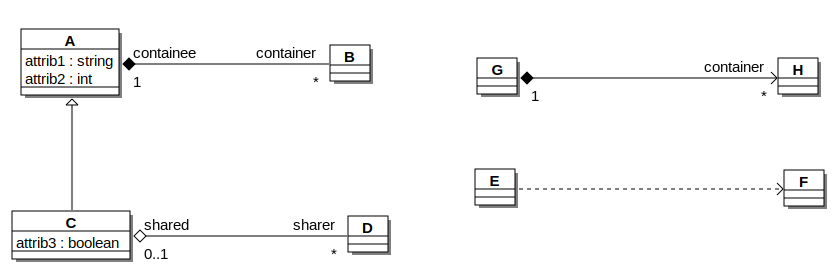
\includegraphics[width=0.9\textwidth]{images/exampleuml}
\caption{An example of the UML elements used in this
  specification. The diagram is explained more fully in the text.}
\label{fig:techref:umlexample}
\end{center}
\end{figure}
%
The UML class diagrams look like the examples in
figure \ref{fig:techref:umlexample}. Again as an aid to
understanding their meanings are described below:
\begin{description}
\item[class] See above for definition. The class symbol displays each
  attribute and its type using the convention: ``attribute : type''.
\item[generalisation (open triangle arrowhead)] Defines an inheritance
  relationship where class C inherits the attributes, associations and
  semantics of class A. This means that C also has attributes
  \attrib{attrib1} and \attrib{attrib2} as well as an association
called \attrib{container} to class B.
\item[composite aggregation (black diamond)] The aggregating class
  (A) is the one adjacent to the diamond and at the other end is the
  contained class (B). This represents a whole/part
  relationship where class B is part of class A and B cannot exist
  independently of A. The cardinality and role of a given class are
  shown at the opposite end of the association to it.
\item[shared aggregation (open diamond)] The aggregating class (C) is
  adjacent to the diamond and is connected to the other class (D) via
  a solid line. Here there is a whole/part relationship, but there the
  part (class D) can be shared with another class and can exists
  independently of C.
\item[navigability (black diamond anchor arrowhead)] If the association ends in an arrow, this
  indicates the direction of the association. Here this should be
  taken to mean that only one aside of the association (G) is `aware' of the relationship.
\item[dependency] Indicates that the dependent class (E) requires the
  other class adjacent to the arrow head (F) to satisfy its
  specification or implementation.
\end{description}
%
The specification uses a number of primitive types that are used in
attribute definitions. These are:
\begin{description}
\item[int] An integer.
\item[string] A string of UniCode characters.
\item[boolean] A Boolean value that can be either True or False.
\item[object] A type that can be any value.
\item[cv] A controlled vocabulary (see \ref{sec:techref:CVs}).
\item[enum] A value that must be chosen from on of an enumerated set
  of predefined values.
\end{description}


\subsection{Definition format}

To help you read the definitions each one follows a standard format
which each section found in the same order.  Sections that are not
relevant are omitted.

\begin{description}
\item[Generalisation]  This section defines the inheritance relationship(s) between this
class and any other classes.
\item[Attributes] Here any attributes specific to this class are defined and their
meaning or purpose described. Attributes from superclasses are part of
this classes definition but are not defined here explicitly.
\item[Associations] Any associations are defined and described. Again associations from
superclasses are not included here, but are part of this classes
definition.
\item[Unique Key] The attributes that together uniquely identify the
  \PD element or concept. If this is ommited then there is no unique
  key. See section~\ref{sec:techref:uniquenessdefinition} for more
  information about identity and uniqueness.
\item[Rules and Constraints] The semantics of the class are defined
  here in the form of itemised rules and constraints on the behaviour
  of the class that are not expressed in the UML definition or other
  parts of the definition.
\item[Notation] If the class corresponds to one or more glyphs then each glyph is
described here. The glyph is described in words and graphically. In
cases where several glyphs combine in complex ways usage examples are
provided.
\item[Layout Rules and Guidelines] In some cases the graphical layout of a glyph and is more complicated
and requires some additional explanation. If this is the case this
will be provided here.
\item[Changes from Previous Version] In order to help track changes between versions of the specification
this section documents where this class definition differs from
that in previous versions. Where appropriate ticket numbers for bugs
or issues addressed in this version should be included.
\end{description}


\begin{sidewaysfigure}
% \begin{figure}[htb]
% \begin{center}
% \begin{sideways}
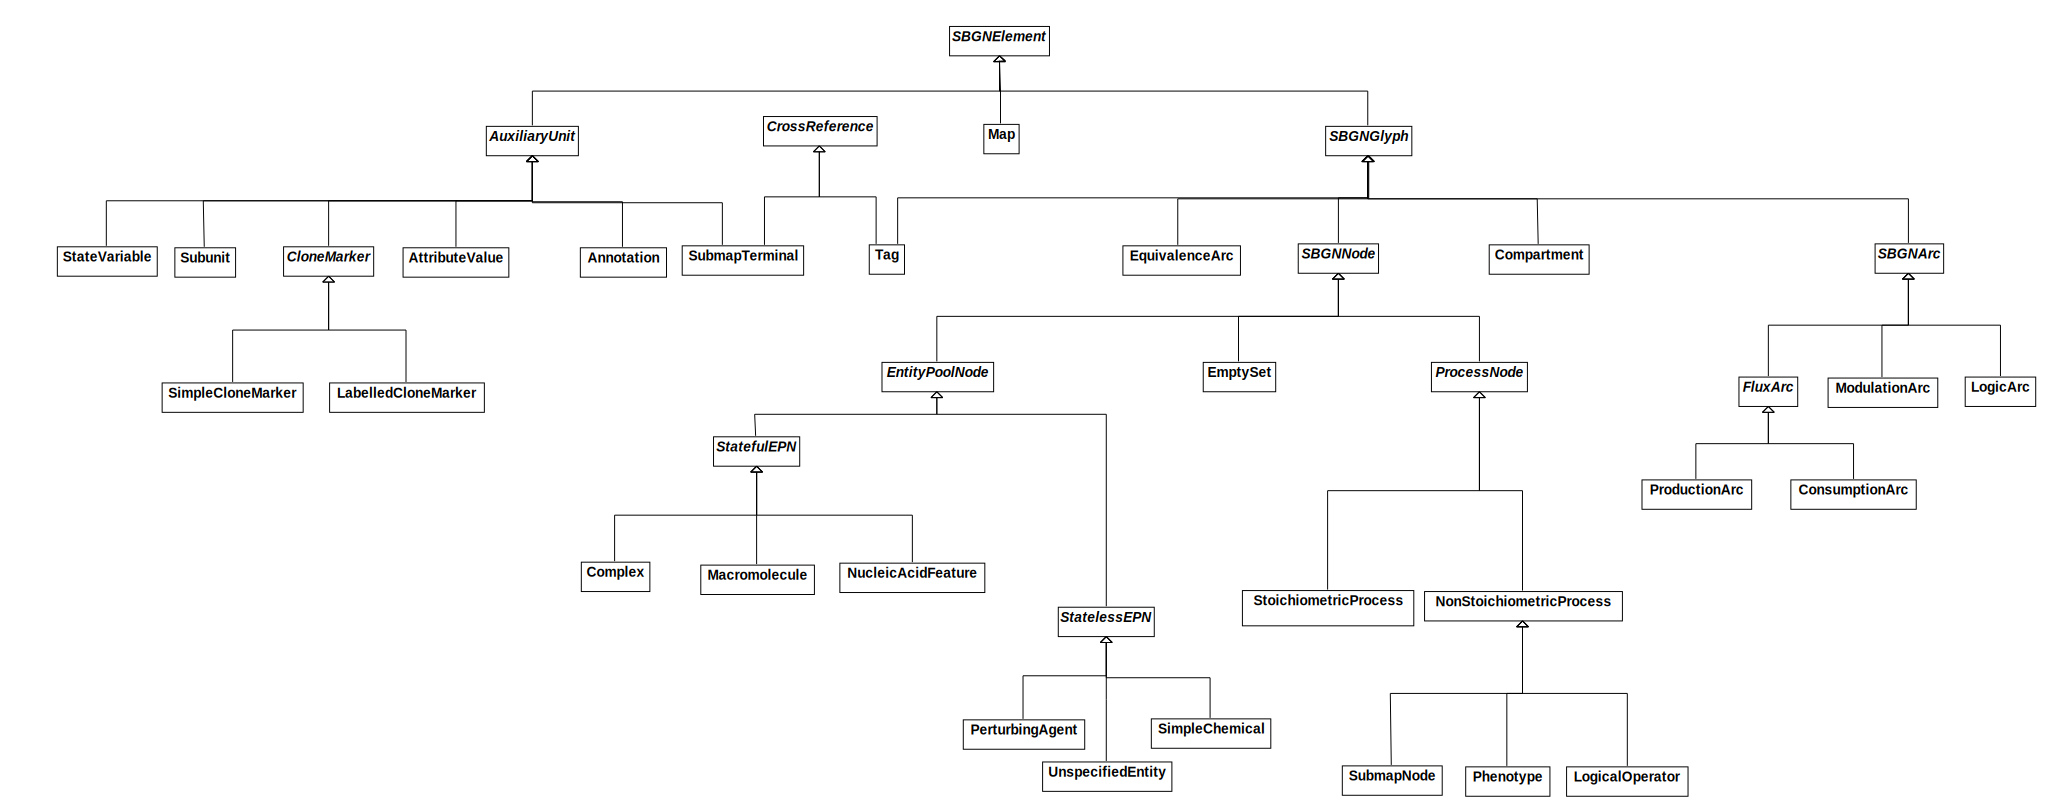
\includegraphics[width=\textheight]{images/sbgnumloverview}
%\end{sideways}
\caption{A view of the UML model describing \PDl. This diagram shows
  the classes and their inheritance relationships. No attributes or
  associations between classes are shown to simplify the
  diagram. These details are provided in the UML class diagrams
  associated with most class definitions.}
\label{fig:techref:sbgnoverviewuml}
% \end{center}
% \end{figure}
\end{sidewaysfigure}

\section{Overview of UML Description}

The complete UML model describing the \PDl is shown in figure
\ref{fig:techref:sbgnoverviewuml}. Care has been taken to try and
represent the key concepts on the \PDl while keeping the model as
simple as possible, for example by minimising the use of multiple
inheritance.

The model has a root class, \sbgnclass{SBGNElement}, that all language
elements inherit from. The nodes and arcs (edges) of the graph
structure inherent in the language are represent by the
\sbgnclass{SBGNNode} and \sbgnclass{SBGNArc} classes. All graphical
elements that can be drawn directly onto a \PDm are glyphs
(\sbgnclass{SBGNGlyph}) and all those that decorate glyphs are
auxiliary units (\sbgnclass{AuxiliaryUnit}). From there the model
captures the organisation of glyphs in to the Entity Pool Nodes
(\sbgnclass{EntityPoolNode}) and Process Nodes
(\sbgnclass{ProcessNode}) familiar in previous versions of the \PDl
specification.  In most cases 'leaf' classes (those without any
subclasses) correspond to the glyphs of the language and in all cases
non-leaf classes are concepts the define the syntax and semantics of
one or more glyphs.

% There are a number of
% language rules that the model and the individual class specification
% cannot capture and these are dealt with later in the chapter after the
% class definitions in section \ref{sec:techref:definitions}.

\section{Definitions}
\label{sec:techref:definitions}

\subsection{SBGNElement}
\label{defn:SBGNElement}

All the glyphs in \SBGNPDLone inherit from
\sbgnclass{SBGNElement}\query{A new concept}. This is an abstract or conceptual class that
helps organise \PD conceptually. \sbgnclass{SBGNElement} (figure
\ref{fig:techref:mapuml}) has a single attribute \attrib{id} that is an
identifying attribute. This means that all SBGN elements defined here,
which ultimately extend \sbgnclass{SBGNBase}, can all be uniquely
identified from each other. This makes sense if you think that a glyph
drawn on a map is distinct from another glyph drawn on the map. The
\attrib{id} attribute reflects this and is not shown explicitly in a
\PDm.

\subsubsection{Generalisation}

None

\subsubsection{Attributes}

\begin{attributes}
  \attitem{id}{identifier}{R} uniquely identifies all SBGN elements in
  the same namespace\query{Not defined previously, but doesn't change
    \PD semantics. reinforces the idea of instance identity that
    exists for all glyphs.}.
\end{attributes}

\subsubsection{Changes from Previous Version}

Not defined in the previous version.

\subsection{Map}
\label{defn:Map}\label{sec:techref:map}


\begin{figure}[htb]
  \centering
  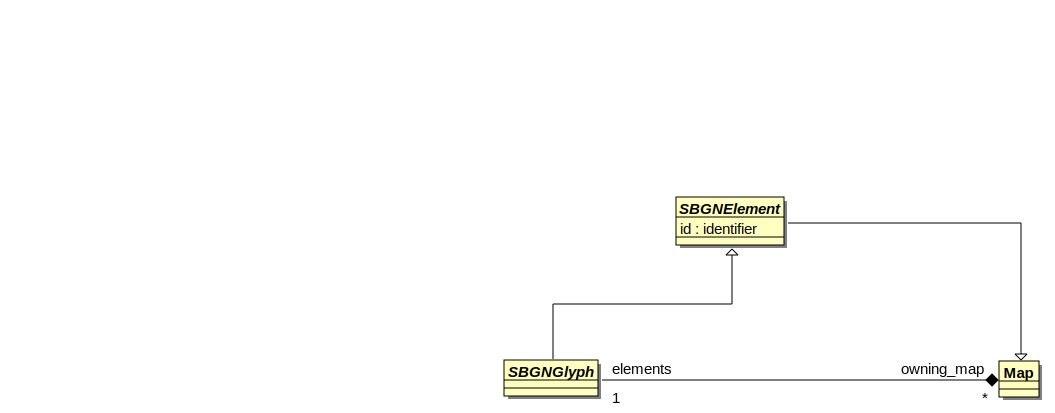
\includegraphics[width=0.55\textwidth]{images/mapuml}
  \caption{UML definition of Map and \sbgnclass{SBGNElement}.}
  \label{fig:techref:mapuml}
\end{figure}

The \sbgnclass{Map}\query{Defining this explicitly is new, but the
  concept of the map as a container of glyphs has always existed in
  the \PDl} (figure \ref{fig:techref:mapuml}) is a container that
holds all the glyphs (\classref{SBGNGlyph}) drawn in a \PDm. A map may
represent a submap or a supermap and should comply with the rules set
out in section \ref{sec:techref:mapsubmaps}. The \attrib{elements} held should be
logically unique and conform to the identity rules in section
\ref{sec:techref:uniquenessdefinition}.


\subsubsection{Generalisation}

\begin{itemize}
\item \classref{SBGNElement}
\end{itemize}

\subsubsection{Attributes}

No additional attributes

\subsubsection{Associations}

\begin{attributes}
\associtem{elements}{SBGNGlyph}{*} The collection of glyphs held by the map.
\end{attributes}

\subsubsection{Rules and Constraints}

\begin{itemize}
\item A map is valid if it is empty (although not very useful).
\item All instances of \classref{SBGNGlyph} must be unique (see
  section \ref{sec:techref:uniquenessdefinition}).
\end{itemize}

\subsubsection{Notation}

The map is the canvas upon which the \PDl is drawn. It's only visible
feature is its colour. It can take any pattern or colour (or be
transparent for that matter), but as SBGN is `colour blind' this does
not convey any meaning in itself.

\subsubsection{Changes from Previous Version}

Not defined explicitly in previous versions.

\subsection{SBGNGlyph}
\label{defn:SBGNGlyph}

\begin{figure}[htb]
  \centering
  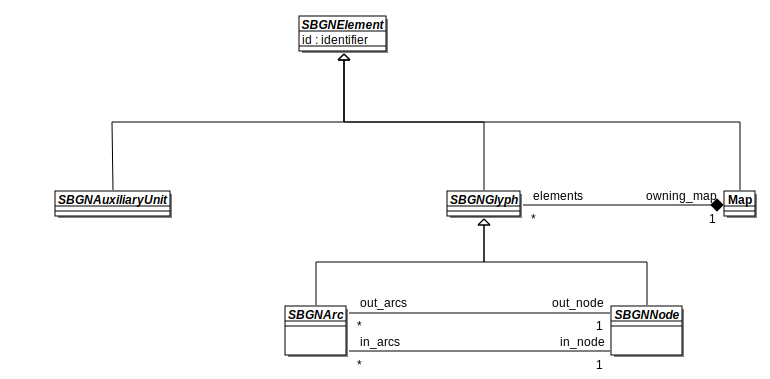
\includegraphics[width=0.9\textwidth]{images/glyphauxuml}
\caption{UML definition of the \sbgnclass{SBGNGlyph} and its subclasses.}
  \label{fig:techref:glyphauxuml}
\end{figure}

The \sbgnclass{SBGNGlyph} is the fundamental building blocks of the
\PDl. It is the only element that can be drawn directly on a map
(\classref{Map}).

\subsubsection{Generalisation}

\begin{itemize}
\item \classref{SBGNElement}
\end{itemize}

\subsubsection{Attributes}

No additional attributes.

\subsubsection{Associations}

\begin{attributes}
\associtem{owning\_map}{Map}{1} The map that contains this class.
\end{attributes}

\subsubsection{Rules and Constraints}

No additional rules and constraints.

\subsubsection{Changes from Previous Version}

Not defined in  previous version.


\subsection{AuxiliaryUnit}
\label{defn:AuxiliaryUnit}

\begin{figure}[htb]
  \centering
  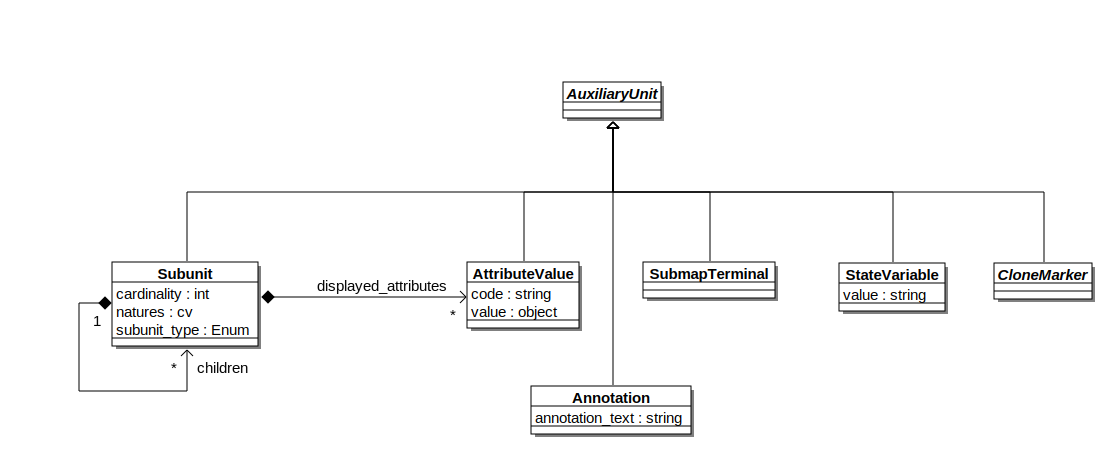
\includegraphics[width=0.75\textwidth]{images/auxiliaryunituml}
\caption{UML definition of the Auxiliary Unit and its subclasses.}
  \label{fig:techref:auxiliaryunituml}
\end{figure}

 The \sbgnclass{AuxiliaryUnit} (figure \ref{fig:techref:auxiliaryunituml}) represents symbols that may be used to
adorn glyphs. In doing so they change the meaning of the glyph and/or provide
additional information about it.

\subsubsection{Generalisation}

\begin{itemize}
\item \classref{SBGNElement}
\end{itemize}

\subsubsection{Attributes}

No additional attributes.

\subsubsection{Associations}

No additional associations.

\subsubsection{Rules and Constraints}

No additional rules and constraints.

\subsubsection{Changes from Previous Version}

Not defined in previous version.


\subsection{SBGNNode}
\label{defn:SBGNNode}

The \sbgnclass{SBGNNode} (figure \ref{fig:techref:sbgnnodearcuml}) represents
the nodes in the graph structure that is the core representation
within the \PDl. The nodes are connected to glyphs descended from
\sbgnclass{SBGNArc} for form a direct graph.

\begin{figure}[htb]
  \centering
  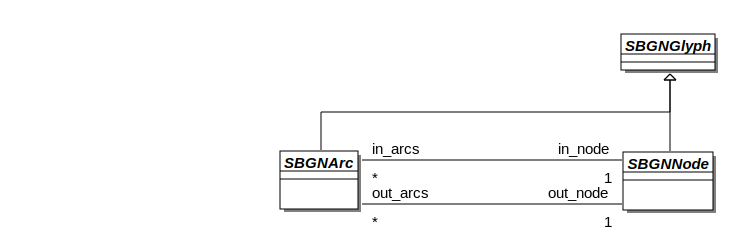
\includegraphics[width=0.55\textwidth]{images/sbgnnodearcuml}
\caption{UML definition of the \sbgnclass{SBGNNode} and
  \sbgnclass{SBGNArc} classes.}
  \label{fig:techref:sbgnnodearcuml}
\end{figure}

\subsubsection{Generalisation}

\begin{itemize}
\item \classref{SBGNGlyph}
\end{itemize}

\subsubsection{Attributes}

No additional attributes.

\subsubsection{Associations}

\begin{attributes}
  \associtem{out\_arcs}{SBGNArc}{*} The arcs leaving this node.
  \associtem{in\_arcs}{SBGNArc}{*} The arcs entering this node.
\end{attributes}

\subsubsection{Rules and Constraints}

\begin{itemize}
\item The set of \sbgnclass{SBGNNode}s linked to this node via a
  \sbgnclass{SBGNArc} (its adjacent nodes) must be all belong to
  different entity pools (as defined by \sbgnclass{EntityPoolNode}).
\end{itemize}

\subsubsection{Changes from Previous Version}

Not defined in the previous version.

\subsection{SBGNArc}
\label{defn:SBGNArc}

The \sbgnclass{SBGNArc} (figure \ref{fig:techref:sbgnnodearcuml}) represents
the directed arcs (also know as directed edges) in the directed graph
structure that is the core representation within \PDl. The arc is
connected to two nodes descended from \sbgnclass{SBGNNode}, one at
each end. As the arc has a direction these nodes are by convention
designated the \attrib{out\_node} to indicate the nodes that the arc
is leaving and \attrib{in\_node} to indicate the node that it is
entering.

\subsubsection{Generalisation}

\begin{itemize}
\item \classref{SBGNGlyph}
\end{itemize}

\subsubsection{Attributes}

No additional attributes.

\subsubsection{Associations}

\begin{attributes}
  \associtem{out\_node}{SBGNNode}{1} The node this arc is leaving.
  \associtem{in\_node}{SBGNNode}{1} The node this arc is entering.
\end{attributes}

\subsubsection{Rules and Constraints}

No additional rules and constraints.

\subsubsection{Changes from Previous Version}

Not defined in the previous version.


\subsection{EntityType}
\label{defn:EntityType}

\begin{figure}[htb]
  \centering
  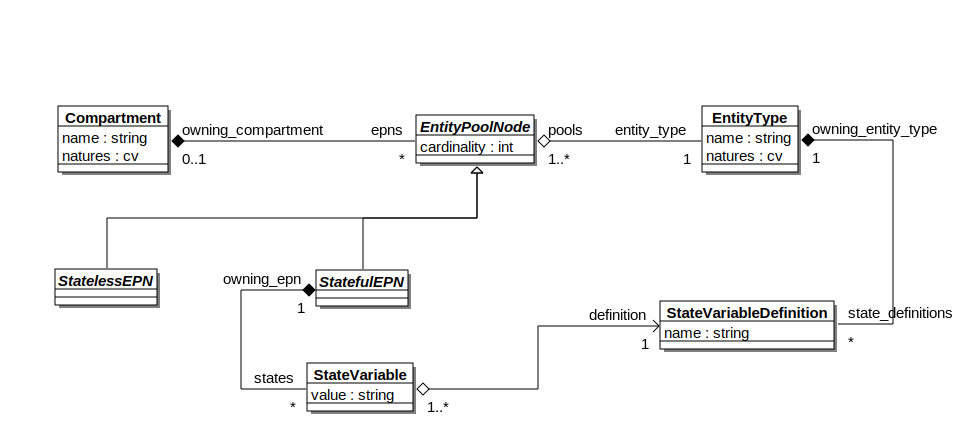
\includegraphics[width=0.85\textwidth]{images/entitytypeuml}
\caption{UML definition of the entity type and the state variable
  definition. The diagram shows how these classes interact with the
  entity pool, state variable and so influence
  \sbgnclass{EntityPoolNode} logical identity.}
  \label{fig:techref:entitytypeuml}
\end{figure}

The \sbgnclass{EntityType}\query{The concept of an entity pool's type
  has been there implicitly in previous versions and comes up in
  discussions. This class aims to formalise that concept and the rules
  associated with it and enable us to formalise rules associated with
  EPNs.} defines the type of entity instantiated by one or more Entity
Pools in a \PDm. The \sbgnclass{EntityType} has associated state
variable definitions (see figure \ref{fig:techref:entitytypeuml}) and
this enforces one of the core rules in the \PDl that once a state is
associated with an entity type it must be used by all entity pools of
that type.


\subsubsection{Generalisation}

None.

\subsubsection{Attributes}

\begin{attributes}
  \attitem{name}{string}{R} The name that identifies the entity in the
  \PDm. EPNs with the same label should be from the same entity. The
  string cannot be empty and must start and end with a non-space
  character. Any Unicode character is acceptable\query{Not discussed
    or defined anywhere, but would make sense to define this explicitly.}.
  \attitem{natures}{cv}{*} The nature of the entity pool node as defined
  by a controlled vocabulary. Zero, one or more values may be set, but
  each one must belong to a different controlled vocabulary (see
  section \ref{sec:techref:CVs})\query{This has been discussed on the mailing
    list where this seems to be the consensus solution}.
\end{attributes}


\subsubsection{Associations}

\begin{attributes}
  \associtem{state\_definitions}{StateVariableDefintion}{*} The state
  definitions associated with this type.
\associtem{pools}{EntityPoolNode}{1..*} The entity pool nodes that
used this type.
\end{attributes}

\subsubsection{Unique Key}

\begin{logicalkey}
  \item \attrib{name}
  \item \attrib{natures}
\end{logicalkey}

\subsubsection{Rule and Constraints}

\begin{itemize}
\item All instances of \sbgnclass{EntityPoolNode} associated with a
  particular \sbgnclass{EntityType} must be of the same class.
\item If an instance of \sbgnclass{EntityType} contains one or more
  instances of \sbgnclass{StateVariableDefinition} then the
  \sbgnclass{EntityPoolNode}s associated with it must be subclasses of
  \sbgnclass{StatefulEPN}.
\end{itemize}

\subsubsection{Notation}

Although there is no direct graphical representation of this class,
other classes that have a composite aggregation with it will need to
represented the \attrib{natures} of the type graphically. Because this
attribute is of class \sbgnclass{AttributeValue} each nature is shown
as a separate \glyph{Unit of Information}. 

% It is shown as a 
% \sbgnclass{AttributeValue} is 
% appearance of the \sbgnclass{AttributeValue} and its associated glyph
% the \glyph{Unit of Information} us common to all subclasses so it is
% convenient to describe it here. The \sbgnclass{AttributeValue} can be
% used to present the \attrib{cardinality} and \attrib{natures} of an
% EPN subclasses. These used the following codes to indicate which attribute
% is being presented:

% \begin{center}
%   \begin{itemize}\setlength{\parskip}{0ex}
%   \item[\texttt{pc}] container physical characteristic
%   \item[\texttt{mt}] entity pool material type
%   \item[\texttt{ct}] entity pool conceptual type
%   \item[\texttt{N}]  multimer cardinality
%   \end{itemize}
% \end{center}



\subsubsection{Changes from Previous Version}

Although not defined explicitly in the previous version, this concept
and the associated rules did exist in the language.

\subsection{StateVariableDefinition}
\label{defn:StateVariableDefinition}

The \sbgnclass{StateVariableDefinition}\query{As with EntityType this
  is new and aims to formalise the concept that an entity pool must
  preserve the same state variables whenever it is used.} defines the state variables
used by an \sbgnclass{EntityType} and therefore those state variables
that must exists in an \sbgnclass{EntityPoolNode} (see figure
\ref{fig:techref:entitytypeuml}).

\subsubsection{Generalisation}

None.

\subsubsection{Attributes}

\begin{attributes}
  \attitem{name}{string}{O} The name that of the state variable. This
  is optional, but if defined cannot be an empty string or just white
  space characters. It should also start with an alpha-numeric
  character and  end with a non-space character. It should not contain
  a `@' character\query{No rule defined previously, but this would
   seem to make sense.}.
\end{attributes}


\subsubsection{Associations}

\begin{attributes}
  \associtem{owning\_entity\_type}{EntityType}{1} The
  \sbgnclass{EntityType} that owns this definition.
\end{attributes}

\subsubsection{Rule and Constraints}

None.

\subsubsection{Changes from Previous Version}

Although not defined explicitly in the previous version, arguably this
concept did exist in the language.

\subsection{EntityPoolNode}
\label{sec:techref:EPNs}\label{defn:EntityPoolNode}\label{sec:techref:EPN}

An entity pool is a population of entities that cannot be
distinguished from each other, when it comes to the \SBGNPDLone
map. For instance all the molecular entities that fulfill the same
role in a given process form an entity pool. As a result, an entity
pool can represent different granularity levels, such as all the
proteins, all the instances of a given protein, only certain forms of
a given protein. To belong to a different compartment is sufficient to
belong to different entity pools. Calcium ions in the endoplasmic
reticulum and calcium ions in the cytosol belong to different entity
pools when it comes to representing calcium release from the
endoplasmic reticulum.

\begin{figure}[htb]
  \centering
  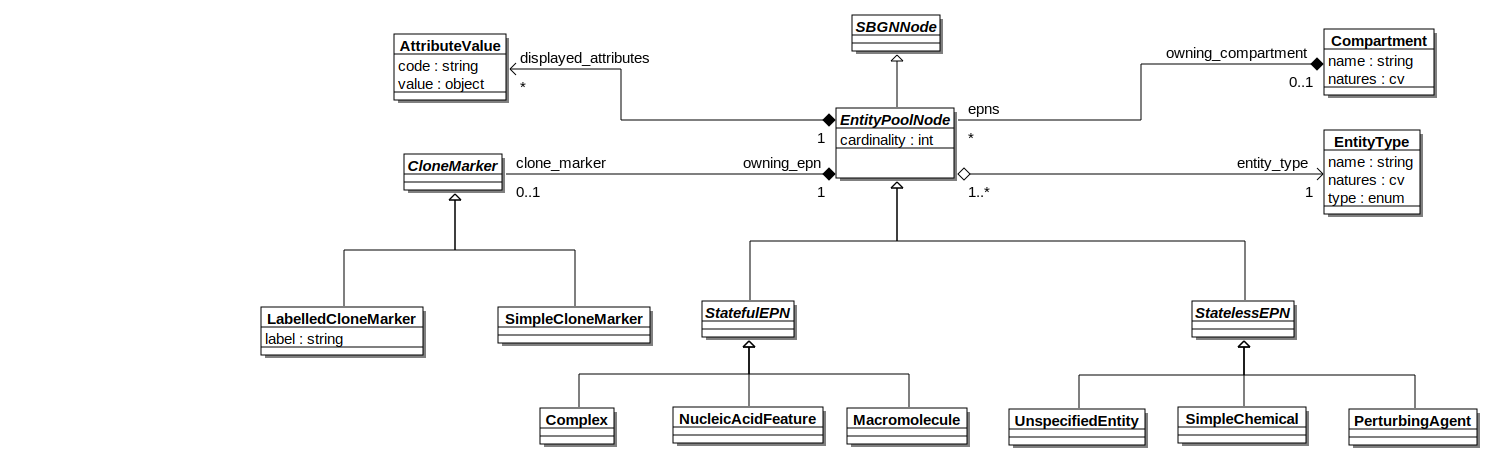
\includegraphics[width=0.85\textwidth]{images/epnuml}
\caption{UML definition of the entity pool node and its descendant glyphs.}
  \label{fig:techref:epnuml}
\end{figure}

The \sbgnclass{EntityPoolNode} (figure \ref{fig:techref:epnuml}) is the
definition of the entity pool and it shares an \sbgnclass{EntityType}
with other identical entities\query{Although this concept is discussed
it is not explicitly defined previously.}. An instance of an entity pools is
therefore distinguished from other pools with the same entity type by
its \attrib{cardinality}, its \attrib{owning\_compartment} and the
\attrib{value}s of its \sbgnclass{StateVariable}s (where
appropriate). It must belong to a compartment or be associated with
the map (c.f.\, section \ref{sec:techref:compartment}) and can contain a clone
marker if it is cloned (see section \ref{sec:techref:epnuniqueness})--- note
that not all EPNs can be cloned.

\subsubsection{Generalisation}

\begin{itemize}
\item \classref{SBGNNode}
\end{itemize}

\subsubsection{Attributes}

\begin{attributes}
  \attitem{cardinality}{int}{R} The number of copies of the entity. Must
  be a positive non-zero integer.
\end{attributes}

\subsubsection{Associations}

\begin{attributes}
 \associtem{owning\_compartment}{Compartment}{0..1} The compartment
  that this EPN belongs too.
\associtem{entity\_type}{EntityType}{1} The type of this entity pool.
  \associtem{clone\_marker}{CloneMarker}{0..1} The clone marker
  decorator. See section \ref{sec:techref:cloneMarker} for its use.
 \associtem{displayed\_attributes}{AttributeValue}{*} One or
 more decorators used to display attribute values\query{This is an
   alternate way of using the Unit of Information to display
   information, but to constrain it so that it presents attributes of
   the EPN not general annotation. See the AttributeValue class for
   more information.}.
\end{attributes}

\subsubsection{Unique Key}

\begin{logicalkey}
\item \attrib{owning\_compartment}
\item \attrib{entity\_type}
\item \attrib{cardinality}
\end{logicalkey}

\subsubsection{Rules and Constraints}

\begin{itemize}
\item If \attrib{cardinality} $>1$ then the descendant glyph must be displayed
  as a multimer.
\item If the EPN is drawn directly on a \glyph{Map} then
  \attrib{owning\_compartment} is not set. We interpret this as
  belonging to an invisible default compartment.
 \item \attrib{natures} can only use the material type (section
 \ref{sec:techref:material-types-cv}), conceptual type (section \ref{sec:techref:conceptual-types-cv}) or physical
 characteristics (section \ref{sec:techref:physical-characteristics-cv}) controlled vocabularies.
\item The appropriate subclass of \sbgnclass{CloneMarker} must be used
  to distinguish logically identical instances of this class.
\item All \sbgnclass{StateVariableDefinition}s associated with the
  \sbgnclass{EntityType} must have an associated
  \sbgnclass{StateVariable}.
\end{itemize}

% \subsubsection{Notation}

% Although there is no direct graphical representation of this class,
% its subclasses all share the same rules for how the cardinality is
% represented graphically. It is shown as a 
% \sbgnclass{AttributeValue} is 
% appearance of the \sbgnclass{AttributeValue} and its associated glyph
% the \glyph{Unit of Information} us common to all subclasses so it is
% convenient to describe it here. The \sbgnclass{AttributeValue} can be
% used to present the \attrib{cardinality} and \attrib{natures} of an
% EPN subclasses. These used the following codes to indicate which attribute
% is being presented:

% \begin{center}
%   \begin{itemize}\setlength{\parskip}{0ex}
%   \item[\texttt{pc}] container physical characteristic
%   \item[\texttt{mt}] entity pool material type
%   \item[\texttt{ct}] entity pool conceptual type
%   \item[\texttt{N}]  multimer cardinality
%   \end{itemize}
% \end{center}


\subsubsection{Changes from Previous Version}

Not defined explicitly in the previous version, but the concept of the
EPN and its semantics existed. The main change to previous semantics
is that of the \attrib{natures}, which didn't formally exist before,
but which now must contain a unique set of controlled vocabularies and
is part of the logical key of the \sbgnclass{EntityPoolNode}.

\subsection{Empty Set}
\label{sec:techref:sourceSink}

It is useful to have the ability to represent the creation of an entity or
a state from an unspecified source, that is, from something that one does
not need or wish to make precise.  For instance, in a model where the
production of a protein is represented, it may not be desirable to
represent all of the amino acids, sugars and other metabolites used, or the
energy involved in the protein's creation.  Similarly, we may not wish to
bother representing the details of the destruction or decomposition of some
biochemical species into a large number of more primitive entities,
preferring instead to simply say that the species ``disappears into a
sink''.  Yet another example is that one may need to represent an input
(respectively, output) into (resp. from) a compartment without explicitly
representing a transport process from a source (resp. to a target).

For these and other situations, SBGN defines a single glyph to handle
these situations representing the involvement of an external pool of
entities.  The symbol used in SBGN is borrowed from the mathematical
symbol for ``empty set'', but it is important to note that it does not
actually represent a true absence of everything or a physical
void---it represents the absence of the corresponding structures in
the model, that is, the fact that the external pool is conceptually
outside the scope of the map.

A frequently asked question is, why bother having an explicit symbol at
all?  The reason is that one cannot simply use an arc that does not
terminate on a node, because the dangling end could be mistaken to be
pointing to another node in the map.  This is specially true if the
map is rescaled, causing the spacing of elements in the map to
change.  The availability and use of an explicit symbol for sources and
sinks is critical.

\begin{figure}[htb]
  \centering
  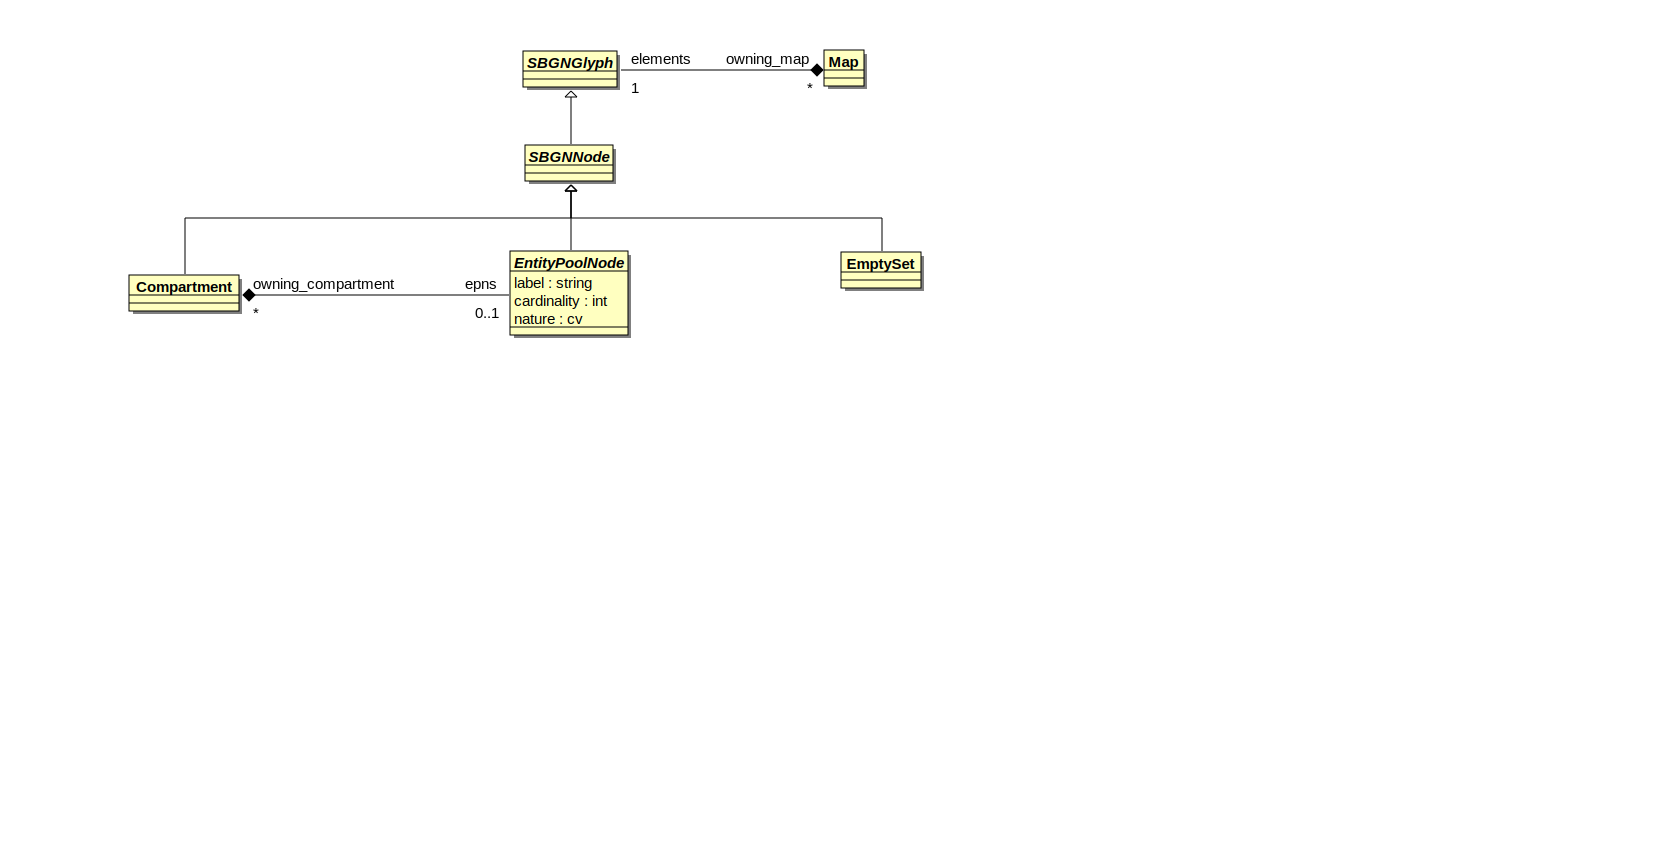
\includegraphics[width=0.75\textwidth]{images/emptysetuml}
  \caption{The UML definition of the \glyph{EmptySet} and its context
    in relation to other elements of the \PDl.}
  \label{fig:techref:emptysetuml}
\end{figure}

The definition of the \glyph{Empty Set} is shown in figure
\ref{fig:techref:emptysetuml}. The empty set is not a subclass of \sbgnclass{EntityPoolNode} as it does not
represent a single pool of entities and does not share any of the
other attributes of an \sbgnclass{EntityPoolNode}, nor does it belong to a particular
compartment\query{This is a significant change to the semantics from
  v1.3 since it is no longer an EPN.}.

\subsubsection{Generalisation}

\begin{itemize}
\item \classref{SBGNNode}
\end{itemize}

\subsubsection{Attributes}

No additional attributes.

\subsubsection{Associations}

No additional associations.

\subsubsection{Rules and Constraints}

\begin{itemize}
\item  All instances of \glyph{Empty Set} can be regarded as identical
therefore no special decoration is used to indicate replication on
the map.
\item the \sbgnclass{EmptySet} must be associated with at least
  one \classref{SBGNArc} (degree $> 0$).
\end{itemize}

\subsubsection{Notation}

\paragraph{Glyph: \glyph{Empty Set}}

\begin{glyphDescription}
\glyphSboTerm SBO:0000291 ! empty set
\glyphContainer Represented by the mathematical symbol for ``empty
set'', that is, a circle crossed by a bar linking the upper-right and
lower-left corners of an invisible square drawn around the circle ($\emptyset$).
\fig{techref:sourceSink} illustrates this.  The symbol should be linked to one
and only one edge in a map.
\glyphLabel None
\end{glyphDescription}

\begin{figure}[htb]
  \centering
  \includegraphics[width = 0.1\textwidth]{images/sourceSink}
  \caption{The \glyph{empty set} glyph.}
  \label{fig:techref:sourceSink}
\end{figure}

\subsubsection{Changes from Previous Version}

The \sbgnclass{EmptySet} and \glyph{Empty Set} glyph has replaced the
\glyph{Source} and \glyph{Sink} glyphs. This symbols used remains the
same, but the underlying concept has changed. The \glyph{Source} and
\glyph{Sink} glyphs where types of EPN, representing single entity
pools, while the \sbgnclass{EmptySet} is not.

\subsection{StatelessEPN}
\label{defn:StatelessEPN}

The \sbgnclass{StatelessEPN} (figure \ref{fig:techref:statelessepnuml})
represents a pool where the entities do not change `state'. In
other-words the entities do not undergo any physical change that is
useful to record in a \PDm. Therefore they cannot be assigned
a state-variable.

\begin{figure}[htb]
  \centering
  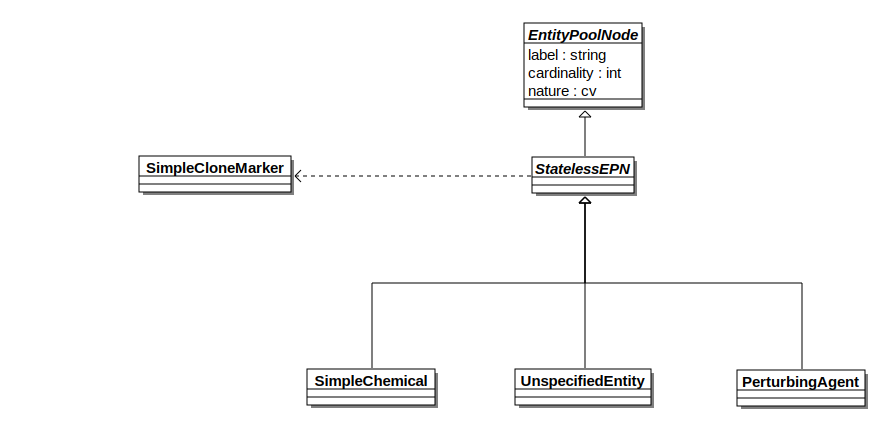
\includegraphics[width=0.75\textwidth]{images/statelessepnuml}
  \caption{UML definition of the stateless entity pool node and its
    descendant glyphs.}
  \label{fig:techref:statelessepnuml}
\end{figure}

\subsubsection{Generalisation}

\begin{itemize}
\item \classref{EntityPoolNode}
\end{itemize}

\subsubsection{Attributes}

No additional attributes.

\subsubsection{Associations}

No additional associations.

\subsubsection{Rules and Constraints}

\begin{itemize}
\item if a clone marker is used it must be of type \sbgnclass{SimpleCloneMarker}.
\end{itemize}

\subsubsection{Changes from Previous Version}

Not defined in the previous version.

\subsection{Simple chemical}
\label{sec:techref:simpleChemical}

A \sbgnclass{SimpleChemical} is the `opposite' of a macromolecule
(\sect{techref:macromolecule}): it is a chemical compound that is \emph{not}
formed by the covalent linking of pseudo-identical residues.  Examples
of simple chemicals are an atom, a monoatomic ion, a salt, a radical,
a solid metal, a crystal, etc.

\subsubsection{Generalisation}

\begin{itemize}
\item \classref{StatelessEPN}
\end{itemize}

\subsubsection{Attributes}

No additional attributes.

\subsubsection{Associations}

No additional associations.

\subsubsection{Rules and Constraints}

No additional rules and constraints.

\subsubsection{Notation}

There are two glyphs associated with \sbgnclass{SimpleChemical}. The
first \glyph{simple chemical monomer} is used when \attrib{cardinality} $= 1$
and the second \glyph{simple chemical multimer} is used when
\attrib{cardinality} $> 1$.

\paragraph{Glyph: \glyph{Simple chemical monomer}}

\begin{glyphDescription}
  \glyphSboTerm SBO:0000247 ! simple chemical \glyphContainer A
  \glyph{simple chemical} is represented by a `stadium' symbol: a
  circle split in two with a rectangle inserted between them (see
  figure \ref{fig:techref:simpleChemical}). If desired the rectangle can have
  zero length and the symbol is then identical to a circle
  (\fig{techref:simpleChemical}). To avoid confusion with the Unspecified
  Entity (\ref{sec:techref:unspecifiedEntity}), this form of the glyph must remain a
  circle and cannot be deformed into an eclipse.

  \glyphLabel The identification of the \glyph{simple chemical} is
  carried by an unbordered box containing a string of characters.  The
  characters may be distributed on several lines to improve
  readability, although this is not mandatory.  The label box has to
  be attached to the center of the circular container.  The label is
  permitted to spill outside the container.
\end{glyphDescription}

\begin{figure}[htb]
  \centering
  
\includegraphics[scale = 0.3]{images/simpleChemical}
  \caption{The \PD glyph for \glyph{simple chemical monomer}. The stadium
    form and circular forms are shown, as are the cloned forms of the glyph.}
  \label{fig:techref:simpleChemical}
\end{figure}

\paragraph{Glyph: \glyph{Simple chemical multimer}}

\begin{glyphDescription}
\glyphSboTerm SBO:0000421 ! multimer of simple chemicals
\glyphContainer  A \glyph{simple chemical multimer} is represented by two identical containers shifted horizontally and vertically and stacked one on top of the other.  \fig{techref:simpleChemicalMultimer} illustrates the glyph.
\glyphLabel The multimer carries an identifying label.  The label is placed in an unbordered box containing a string of characters.  The characters can be distributed on several lines to improve readability, although this is not mandatory.  The label box must be attached to the center of the top monomer's container.  The label may spill outside of the container.
\end{glyphDescription}

\begin{figure}[htb]
  \centering
  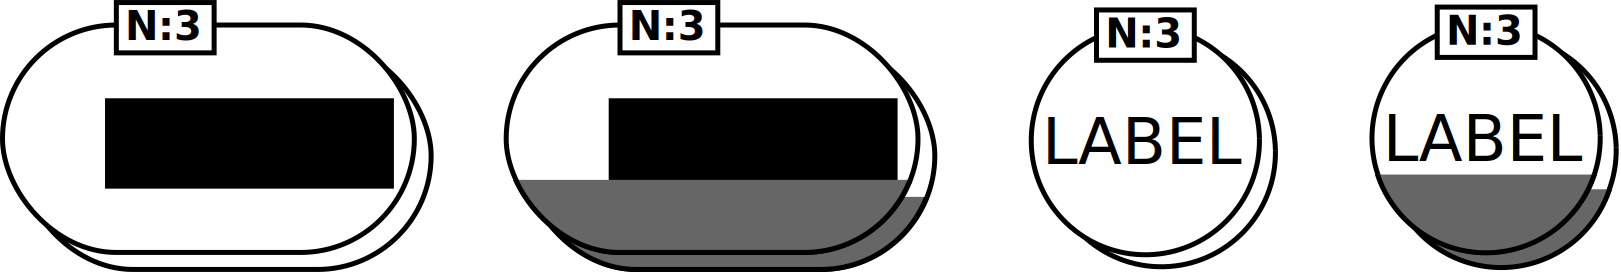
\includegraphics[scale = 0.3]{images/simpleChemicalMultimer}
  \caption{The \PD glyph for \glyph{simple chemical multimer}. The
    figures show the stadium and circular forms, and their cloned variants.}
  \label{fig:techref:simpleChemicalMultimer}
\end{figure}

\subsubsection{Changes from Previous Version}

The glyphs used for the \sbgnclass{SimpleChemical} have been changed
to the stadium glyph. Previously the glyph was a circle. To maintain
compatibility with previous versions the stadium symbol can be drawn
without straight horizontal elements so that it becomes a circle.

\subsection{UnspecifiedEntity}
\label{sec:techref:unspecifiedEntity}

The simplest type of \sbgnclass{EntityPoolNode} is the
\sbgnclass{UnspecifiedEntity} --- one whose type is unknown or simply
not relevant to the purposes of the map.  This arises, for example,
when the existence of the entity has been inferred indirectly, or when
the entity is merely a construct introduced for the needs of a map,
without direct biological relevance.  These are examples of situations
where the \sbgnclass{UnspecifiedEntity} is appropriate.  (Conversely,
for cases where the identity of the entities composing the pool
\emph{is} known, there exist other, more specific glyphs described
elsewhere in the specification.)

\subsubsection{Generalisation}

\begin{itemize}
\item \classref{StatelessEPN}
\end{itemize}

\subsubsection{Attributes}

No additional attributes.

\subsubsection{Associations}

No additional associations.

\subsubsection{Rules and Constraints}

\begin{itemize}
\item The \sbgnclass{UnspecifiedEntity} cannot have cardinality $>
  1$. This means there is no multimer glyph.
\end{itemize}

\subsubsection{Notation}

\paragraph{Glyph: \glyph{Unspecified entity}}

\begin{glyphDescription}
\glyphSboTerm SBO:0000285 ! material entity of unspecified nature
\glyphContainer An \glyph{unspecified entity} is represented by an
elliptic container, as shown in \ref{fig:techref:unspecified}.  Note that this
must remain an ellipse to avoid confusion with the Simple Chemical
glyph, which is a circle (c.f.\, \ref{sec:techref:simpleChemical}).
\glyphLabel An \glyph{unspecified entity} is identified by a label
placed in an unbordered box containing a string of characters.  The
characters can be distributed on several lines to improve readability,
although this is not mandatory.  The label box must be attached to the
center of the container.  The label may spill outside of the
container.
\end{glyphDescription}

\begin{figure}[htb]
  \centering
  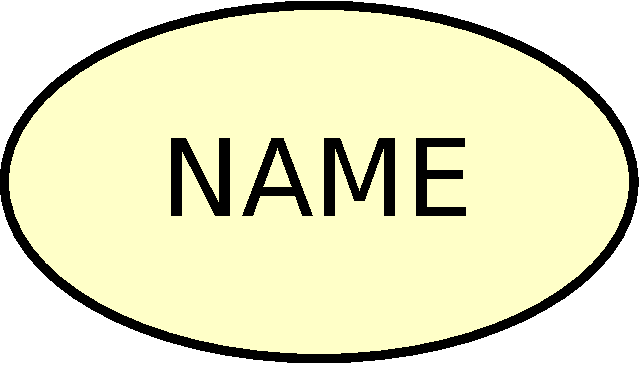
\includegraphics[width=2.5in]{images/unspecified}
  \caption{The \PD glyph for \glyph{unspecified entity}.}
  \label{fig:techref:unspecified}
\end{figure}

\subsubsection{Changes from Previous Version}

No changes from the previous version.

\subsection{Perturbing Agent}
\label{sec:techref:perturbing agent}

Biochemical networks can be affected by external influences.  Those
influences can be the effect of well-defined physical perturbing
agents, such as a light pulse or a change in temperature; they can
also be more complex and not well-defined phenomena, for instance the
outcome of a biological process, an experimental setup, or a mutation.
For these situations, SBGN provides the \glyph{perturbing agent}
glyph. It is an EPN, and represents the amount to perturbing agent
applied to a process.

\subsubsection{Generalisation}

\begin{itemize}
\item \classref{StatelessEPN}
\end{itemize}

\subsubsection{Attributes}

No additional attributes.

\subsubsection{Associations}

No additional attributes.

\subsubsection{Rules and Constraints}

\begin{itemize}
\item The \sbgnclass{PerturbingAgent} cannot have \attrib{cardinality} $>
  1$. This means there is no multimer glyph.
\end{itemize}

\subsubsection{Notation}

\paragraph{Glyph: \glyph{Perturbing agent}}

\begin{glyphDescription}
\glyphSboTerm SBO:0000405 ! perturbing agent
\glyphContainer A \glyph{perturbing agent} is represented by a modified hexagon
having two opposite concave faces, as illustrated in \fig{techref:perturbing agent}.
\glyphLabel A \glyph{perturbing agent} is identified by a label placed in an
unbordered box containing a string of characters.  The characters can be
distributed on several lines to improve readability, although this is not
mandatory.  The label box must be attached to the center of the
\glyph{perturbing agent} container.  The label may spill outside of the container.
\end{glyphDescription}

\begin{figure}[htb]
  \centering
  
\includegraphics[scale = 0.3]{images/perturbing_agent}
  \caption{The \PD glyph for \glyph{perturbing agent}.}
  \label{fig:techref:perturbing agent}
\end{figure}

\subsubsection{Changes from Previous Version}

No changes from pervious version.

\subsection{StatefulEPN}
\label{defn:StatefulEPN}

Stateful entity pools can undergo physical changes, for example
chemical modifcation or conformational change, which we wish to record
in a \PDm. This information is captured via the
\sbgnclass{StateVariable} (as can be seen in figure
\ref{fig:techref:statefulepnuml}). The \sbgnclass{LabellecCloneMarker} must be
used to indicated that the \sbgnclass{StatefulEPN} is cloned.

\begin{figure}[htb]
  \centering
  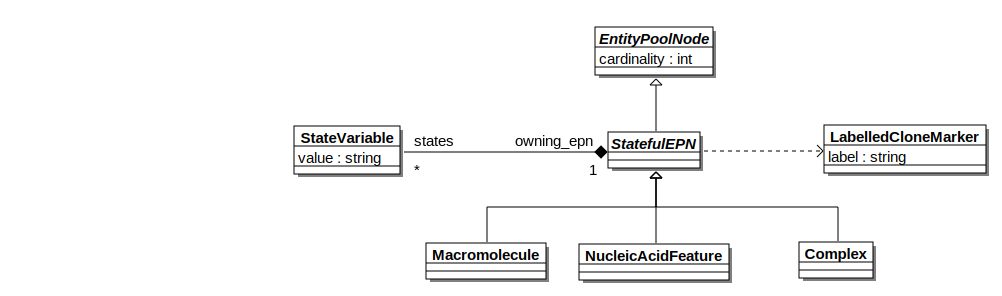
\includegraphics[width=0.75\textwidth]{images/statefulepnuml}
\caption{UML definition of the stateful entity pool node: showing its
  descendants and its association with state variables.}
  \label{fig:techref:statefulepnuml}
\end{figure}

\subsubsection{Generalisation}

\begin{itemize}
\item \classref{EntityPoolNode}
\end{itemize}

\subsubsection{Attributes}

No additional attributes.

\subsubsection{Associations}

\begin{attributes}
\associtem{states}{StateVariable}{*} The state variables
  that belong to this class.
\end{attributes}

\subsubsection{Rules and Constraints}

\begin{itemize}
\item State variables do not need to be logically unique, therefore
  two or more state variables with the same name are permitted.
\item The \sbgnclass{LabelledCloneMarker} must be used to indicate
  cloning for instances of \sbgnclass{StatefulEPN} and its subclasses,
  with a must use the same
\end{itemize}

\subsubsection{Changes from Previous Version}

Not defined explicitly in the previous version.

\subsection{Macromolecule}
\label{sec:techref:macromolecule}

Many biological processes involve \emph{macromolecules}: biochemical
substances that are built up from the covalent linking of
pseudo-identical units.  Examples of macromolecules include proteins,
nucleic acids (RNA, DNA), and polysaccharides (glycogen, cellulose,
starch, etc.).  Attempting to define a separate glyph for all of these
different molecules would lead to an explosion of symbols in SBGN, so
instead, \SBGNPDLone defines only one glyph for all macromolecules.
The same glyph is to be used for a protein, a nucleic acid, a complex
sugar, and so on.  The exact nature of a particular macromolecule in a
map is then clarified using its label and decorations, as will become
clear below.

\subsubsection{Generalisation}

\begin{itemize}
\item \classref{StatefulEPN}
\end{itemize}

\subsubsection{Attributes}

No additional attributes.

\subsubsection{Associations}

No additional associations.

\subsubsection{Rules and Constraints}

No additional rules and constraints.

\subsubsection{Notation}

There are two glyphs associated with \sbgnclass{Macromolecule}. The
first \glyph{Macromolecule monomer} is used when \attrib{cardinality} $= 1$
and the second \glyph{Macromolecule multimer} is used when
\attrib{cardinality} $> 1$.

\paragraph{Glyph: \glyph{Macromolecule monomer}}

\begin{glyphDescription}
\glyphSboTerm SBO:0000245 ! macromolecule
\glyphContainer A macromolecule is represented by a rectangular container with rounded
corners, as illustrated in \fig{techref:macromolecule}.
\glyphLabel A \glyph{macromolecule} is identified by a label placed in an unbordered box containing a string of characters.  The characters can be distributed on several lines to improve readability, although this is not mandatory.  The label box must be attached to the center of the container.  The label may spill outside of the container.
\end{glyphDescription}

\begin{figure}[htb]
  \centering
  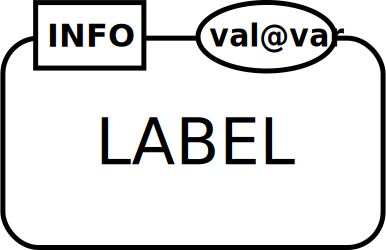
\includegraphics[width = 3.5in]{images/macromolecule}
  \caption{The \PD glyph for \glyph{macromolecule}, shown plain and
    unadorned on the left, and with an additional state variable and a
    unit of information in the middle and the cloned form on the right.}
  \label{fig:techref:macromolecule}
\end{figure}

\paragraph{Glyph: \glyph{Macromolecule multimer}}

\begin{glyphDescription}
\glyphSboTerm SBO:0000420 ! multimer of macromolecules
\glyphContainer A \glyph{multimer} is represented by two identical containers shifted horizontally and vertically and stacked one on top of the other.  \fig{techref:macromolMultimer} illustrates the glyph.
\glyphLabel As monomer
\end{glyphDescription}

\begin{figure}[htb]
  \centering
  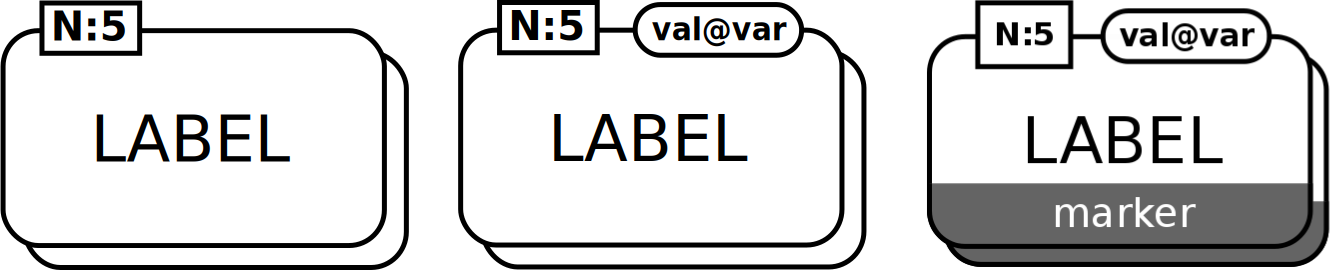
\includegraphics[width = 3.5in]{images/macromolMultimer}
  \caption{The \PD glyph for \glyph{macromolecule multimer}, shown plain and
    unadorned on the left, and with an additional state variable and a
    unit of information in the right and the cloned form on the right.}
  \label{fig:techref:macromolMultimer}
\end{figure}

\paragraph{Usage Examples}
\label{sec:techref:CplxEPNs}

In this section, we provide examples of Entity Pool Node representations drawn using the \SBGNPDLone glyphs described above.

\fig{techref:example-camkii} represents calcium/calmodulin kinase II, with phosphorylation on the sites threonine 286 and 306, as well as catalytic and autoinhibitory domains.  Note the use of \emph{units of information} and \emph{state variables}.

\begin{figure}[htb]
  \centering
  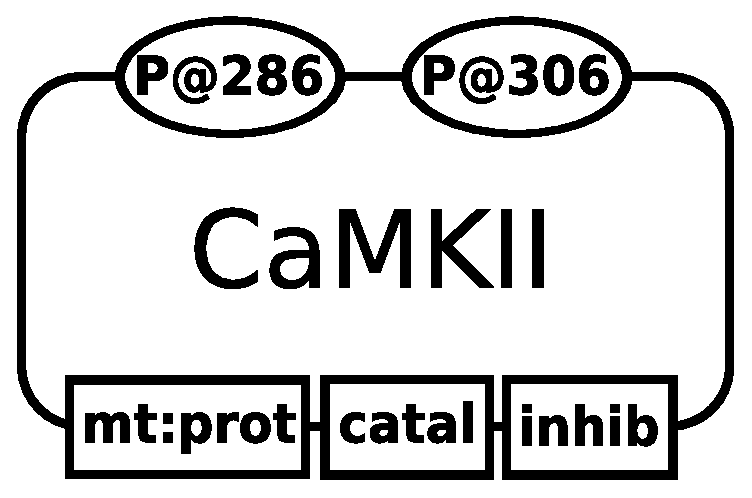
\includegraphics[scale = 0.3]{examples/macromolecule-CaMKII}
  \caption{An example representation of calcium/calmodulin kinase II.}
  \label{fig:techref:example-camkii}
\end{figure}

\fig{techref:example-glur} represents the glutamate receptor in the open state, with both phosphorylation and glycosylation.  The entity carries two functional domains, the ligand-binding domain and the ion pore, and its chemical nature is precided.

\begin{figure}[htb]
  \centering
  \includegraphics[scale = 0.3]{examples/macromolecule-GluR}
  \caption{An example of a glutamate receptor in the open state.}
  \label{fig:techref:example-glur}
\end{figure}


\subsubsection{Changes from Previous Version}

No changes from the previous version.

\subsection{NucleicAcidFeature}
\label{sec:techref:genetic}

The \sbgnclass{NucleicAcidFeature} represents a fragment of a
macromolecule carrying genetic information.  A common use for this
construct is to represent a gene or transcript.  The label of this EPN
and its \attrib{natures} are often important for making the purpose
clear to the reader of a map.

\subsubsection{Generalisation}

\begin{itemize}
\item \classref{StatefulEPN}
\end{itemize}

\subsubsection{Attributes}

No additional attributes.

\subsubsection{Associations}

No additional associations.

\subsubsection{Rules and Constraints}

No additional rules and constraints.

\subsubsection{Notation}

The \sbgnclass{NucleicAcidFeature} has two associated glyphs. The
first \glyph{Nucleic acid feature monomer} is used when
\attrib{cardinality} $=1$ and the second, \glyph{Nucleic acid feature
  multimer} is used when \attrib{cardinality} $>1$.

\paragraph{Glyph: \glyph{Nucleic acid feature monomer}}

This glyphs represents a monomeric macromolecule.

\begin{glyphDescription}
\glyphSboTerm SBO:0000354 !  informational molecule segment
\glyphContainer A \glyph{nucleic acid feature} is represented by a rectangular container whose bottom half has rounded corners, as shown in \fig{techref:genetic}.
\glyphLabel The identity of a particular \glyph{Nucleic acid feature} is established by a label placed in an unordered box containing a string of characters.  The characters may be distributed on several lines to improve readability, although this is not mandatory.  The label box must be attached to the center of the container.  The label may spill outside of the container.
\end{glyphDescription}


\begin{figure}[htb]
  \centering
  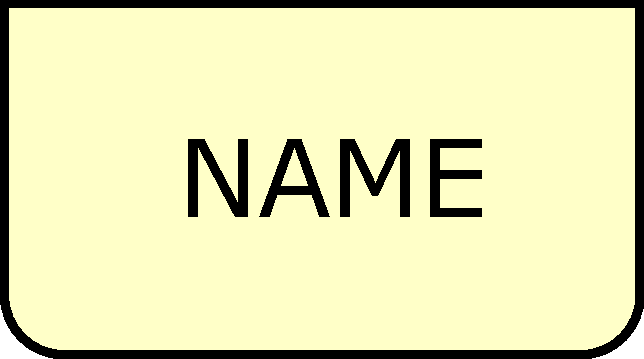
\includegraphics[width = 3.5in]{images/genetic}
  \caption{The \PD glyph for \glyph{nucleic acid feature monomer}, shown plain and
    unadorned on the left and with an additional state variable and a
    unit of information in the middle and the cloned form on the right.}
  \label{fig:techref:genetic}
\end{figure}

\paragraph{Glyph: \glyph{Nucleic acid feature multimer}}

This glyphs represents a multimeric macromolecule.

\begin{glyphDescription}

\glyphSboTerm SBO:0000419 ! multimer of informational molecule segments

\glyphContainer A \glyph{Nucleic acid feature multimer} is represented by two identical containers shifted horizontally and vertically and stacked one on top of the other.  \fig{techref:genetic-multimer} illustrates the glyph.

\glyphLabel As monomer glyph.

\end{glyphDescription}

\begin{figure}[htb]
  \centering
  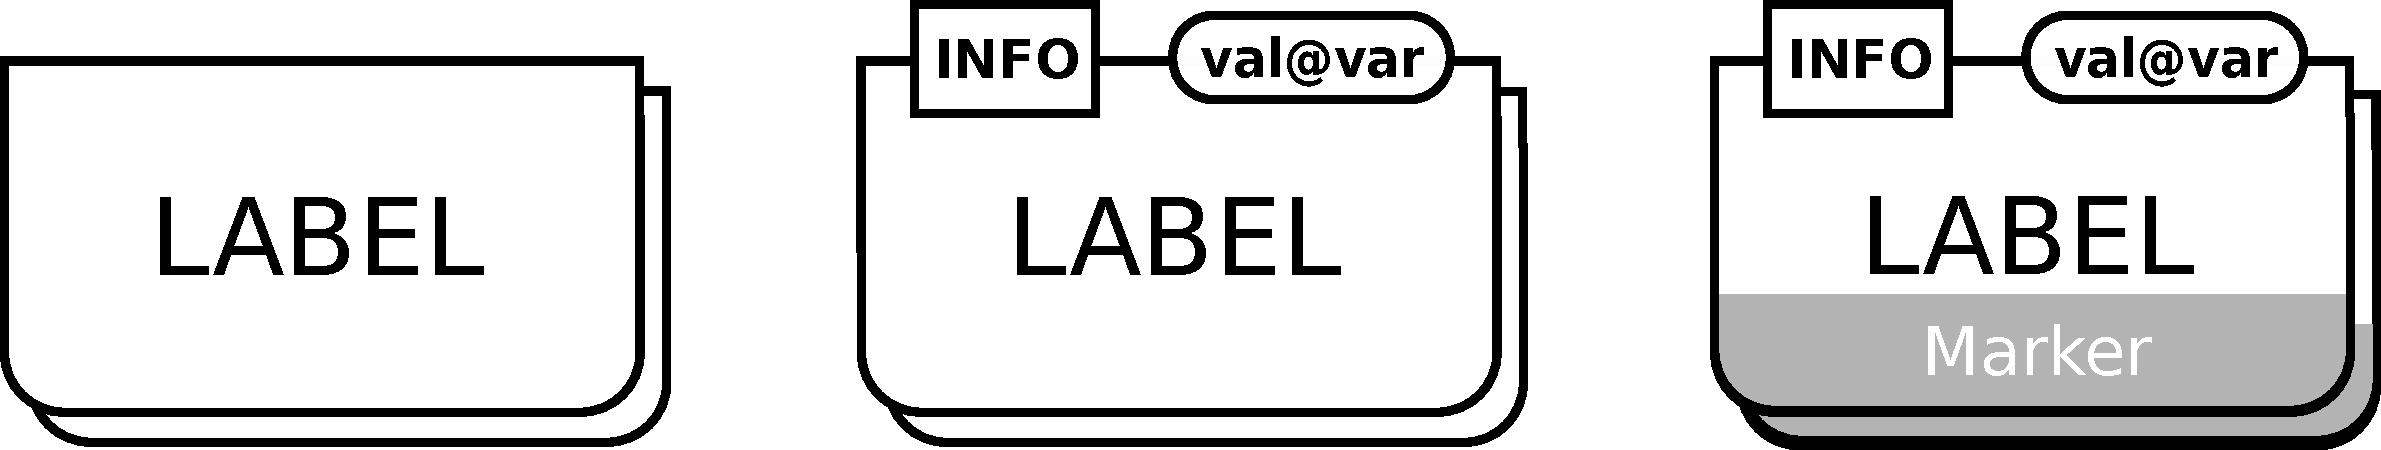
\includegraphics[width = 3.5in]{images/geneticMultimer}
  \caption{The \PD glyph for \glyph{nucleic acid feature multimer}, shown plain and
    unadorned on the left and with an additional state variable and a
    unit of information in the middle and the cloned form on the right.}
  \label{fig:techref:genetic-multimer}
\end{figure}

\subsubsection{Changes from Previous Version}

No changes from the previous version.

%%%%%%%%%%%%%%%%%%%%%%%%%%%%%%%%%%%%%%%%%%%%%%%%%%%%%%%%%%%%%%%%%%%%%%
%%%%                   Complex
%%%%%%%%%%%%%%%%%%%%%%%%%%%%%%%%%%%%%%%%%%%%%%%%%%%%%%%%%%%%%%%%%%%%%%

\subsection{Complex}\label{sec:techref:complex}
\label{defn:Complex}

A \sbgnclass{Complex} represents a biochemical entity composed of
other biochemical entities, whether macromolecules, simple chemicals,
multimers, or other complexes (figure
\ref{fig:techref:complexsubunituml}). The \sbgnclass{Complex} can described
its composition by the set of \sbgnclass{Subunit}s it contains (see
figure \ref{sec:techref:subunits}). This description is entirely optional and
is their to assist the user with a visual shorthand about the
composition of the complex.

\begin{figure}[htb]
  \centering
  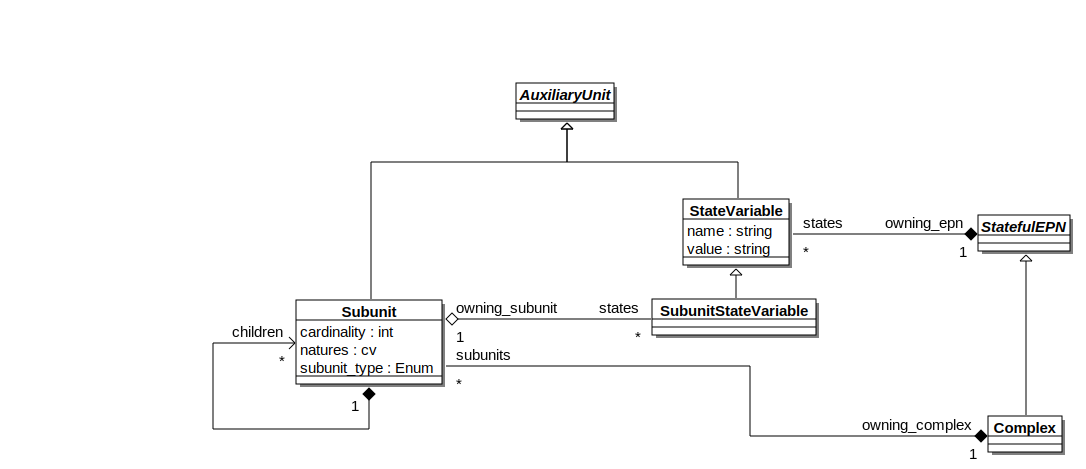
\includegraphics[width = 0.75\textwidth]{images/complexsubunituml}
  \caption{The UML definition of the \sbgnclass{Complex} and its
    associated \sbgnclass{subunit}s. In particular this describes organisation
   of the state variables that belong to both the subunit, but also
   the complex.}
  \label{fig:techref:complexsubunituml}
\end{figure}

\subsubsection{Generalisations}

\begin{itemize}
\item \classref{EntityPoolNode}
\end{itemize}

\subsubsection{Attributes}

No additional attributes

\subsubsection{Associations}

\begin{attributes}
  \associtem{subunits}{Subunit}{*} The subunits that describe
  the composition of this complex.
 \end{attributes}


\subsubsection{Special Rules and Constraints}

\begin{itemize}
\item Once a set of subunits are defined for an \sbgnclass{Complex}
  with a given \sbgnclass{EntityType}, then they must be used by every
  instance using that entity type.\query{New rule.}.
\item The set of subunits in the Complex does not identify it. One or
  more Complexes that contain the same set of subunits, but have
  different labels are \textbf{not} identical.
\end{itemize}

\subsubsection{Notation}

The Complex is represented by two glyphs, the \glyph{Complex Monomer}
which represents a \sbgnclass{Complex} where the \attrib{cardinality}
is one and the \glyph{Complex Multimer} where the cardinality is
greater than that.

\paragraph{\glyph{Complex Monomer}}

\begin{glyphDescription}
\glyphSboTerm SBO:0000253 ! non-covalent complex
\glyphContainer A \glyph{complex} possesses its own container box surrounding the juxtaposed container boxes of its components.  This container box is a rectangle with cut-corners (an octagonal box with sides of two different lengths).  The size of the cut-corners are adjusted so that there is no overlap between the container and the components.  The container boxes of the components must not overlap.
\glyphLabel The identification of a \glyph{named complex} is carried
by an unbordered box containing a string of characters.  The
characters may be distributed on several lines to improve readability,
although this is not mandatory.  Ideally the label box should be
attached to the midway between the border of the complex's container
box and the border of the components' container boxes. However, if the
Complex contains Subunit glyphs then the label may be positions to
optimise the clarity and avoid overlapping.
\end{glyphDescription}

\begin{figure}[htb]
  \centering
  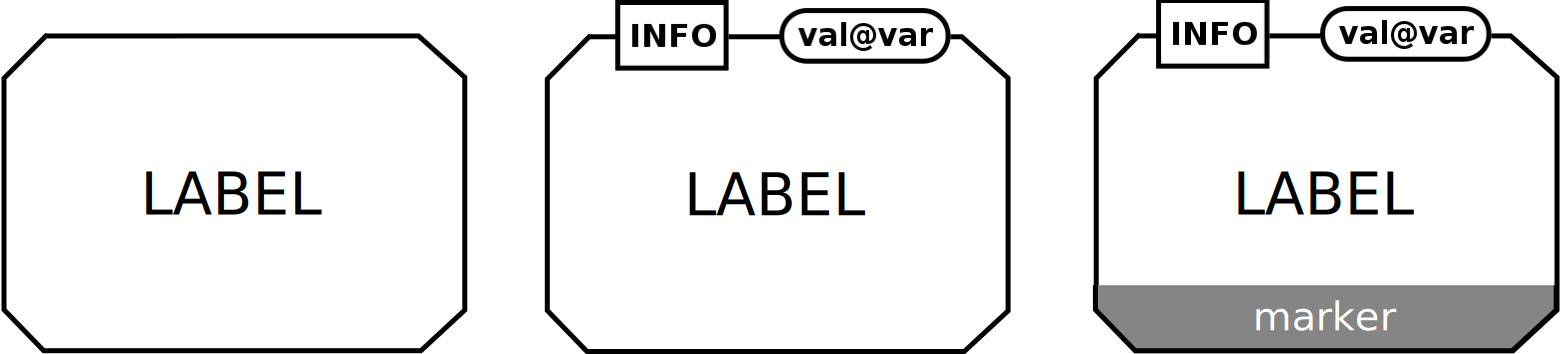
\includegraphics[width=3.5in]{images/complexGlyph}
  \caption{The \glyph{complex} glyph.}
  \label{fig:techref:complex}
\end{figure}


\paragraph{\glyph{Complex Multimer}}

 \begin{glyphDescription}
\glyphSboTerm SBO:0000418 ! multimer of complexes
\glyphContainer A \glyph{Complex Multimer} is represented by two
identical \glyph{Complex} containers shifted horizontally and
vertically and stacked one on top of the other.  \fig{techref:complexMultimer}
illustrates the glyph.
\glyphLabel As monomer
\end{glyphDescription}

\begin{figure}[htb]
  \centering
  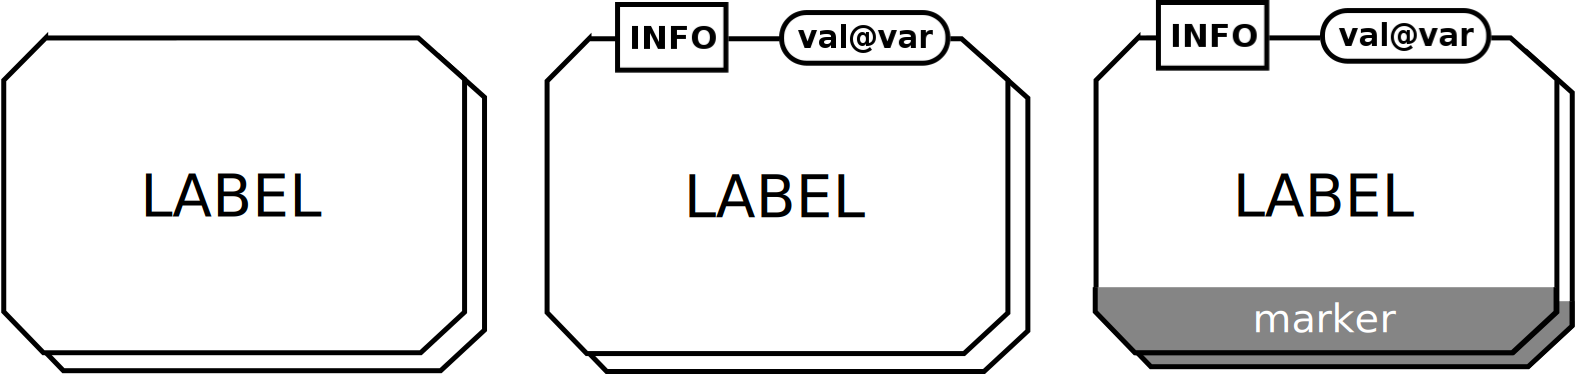
\includegraphics[width = 3.5in]{images/complexMultimerGlyph}
  \caption{The \glyph{Complex Multimer} glyph.}
  \label{fig:techref:complexMultimer}
\end{figure}

\subsubsection{Layout Rules and Guidelines}

\begin{itemize}
\item The subunits inside the complex must not overlap.
\item The subunits should sit above the clone marker so that they are
  not obscured by it.
\item The label should not be obscured by subunits or obscure them.
\end{itemize}


\subsubsection{Changes from Previous Version}

\begin{itemize}
\item Clarified that complex must have a label and the label
  identifies the complex irrespective of its subunit composition.
\item The label positioning does not need to be at the centre of the
  Complex glyph.
\end{itemize}

\subsection{Subunit}
\label{defn:Subunit}\label{sec:techref:subunits}

The \sbgnclass{Subunit}\query{The principles of the subunit have been
  agreed, but the details of this implementation should be
  reviewed. In particular the rules about state variables.} is used to describe the composition of the
\classref{Complex}. A complex can optionally be decorated with one or
more subunits, which represent the types of \classref{EntityPoolNode}
that may aggregate to form a complex. As we can see from the UML
representation (figure \ref{fig:techref:complexsubunituml}) the
\sbgnclass{Subunit} is an auxiliary unit that decorates the
\sbgnclass{Complex} and does not represent an entity pool directly. In
addition it does not mimic the \sbgnclass{EntityPoolNode} class
hierarchy (\sbgnclass{Subunit}, but rather uses the
\attrib{subunit\_type} attribute to indicate the type of subunit.

\subsubsection{Generalisation}

\begin{itemize}
\item \classref{EntityPoolNode}
\end{itemize}

\subsubsection{Attributes}

\begin{attributes}
  \attitem{cardinality}{int}{R} The number of copies of the subunit.
  \attitem{name}{string}{O} The name of the subunit.
  \attitem{subunit\_type}{enum}{R} The type of the subunit. It can have
  one of the following values that correspond to the equivalent EPN
  class: \sbgnclass{SimpleChemical}, \sbgnclass{UnspecifiedEntity},
  \sbgnclass{PerturbingAgent}, \sbgnclass{Macromolecule},
  \sbgnclass{NucleicAcidFeature}, \sbgnclass{Complex}.
\end{attributes}

\subsubsection{Associations}

\begin{attributes}
  \associtem{owning\_complex}{Complex}{1} The complex that owns the subunit.
  \associtem{states}{SubunitStateVariable}{*} The state variables assigned
  to this subunit.
  \associtem{children}{Subunit}{*} Subunits that are contained by this subunit.
\end{attributes}

\subsubsection{Rules and Constraints}

\begin{itemize}
\item Two or more state variables with the same name are
  permitted.
\item State variables with no name set are permitted.
\item Subunits can also contain subunits. There is no limit on such nesting. The namespace rules
  below apply.
\item The subunit defines a namespace for its state variables, e.g.\,
  subunit ``A'' assigned a state variable ``P@Ser202''  and a subunit
  ``B'' assigned the same state variable can be distinguised as
  A:P@Ser202 and B:P@Ser202.
\item If the subunit is of type Complex then \attrib{children} can contain one or
  more \sbgnclass{Subunit} instances.
\item If the subunit has a cardinality $>1$ then this should be
  displayed by the \classref{AttributeValue}.
\item If \attrib{natures} contains one or more instances then these
  must be displayed via an \sbgnclass{AttributeValue}.
\end{itemize}

\subsubsection{Notation}

The subunit symbol used for the \glyph{subunit} glyph varies depending
on the \attrib{subunit\_type} and \attrib{cardinality}. The symbols
available are equivalent to those used by the EPN glyphs including the
\glyph{complex}. Therefore it is possible to describe complexes within
complexes. The mapping between these and the symbol used is shown
in the table below. Not that subunits may contain labels
corresponding to their \attrib{name}.
% \ref{tab:techref:subunit types}

\begin{center}
\begin{tabular}[c]{l l l}\toprule\\
SimpleChemical &  \glyph{Simple Chemical Monomer} & \glyph{Simple
  Chemical Multimer}\\
UnspecifiedEntity & \glyph{Unspecificed Entity} & None\\
PerturbingAgent & \glyph{Perturbing Agent} & None\\
Macromolecule & \glyph{Macromolecule Monomer} &
\glyph{Macromolecule Multimer}\\
Nucleic\-Acid\-Feature & \glyph{Nucleic Acid Feature Monomer} & \glyph{Nucleic Acid Feature Multimer}\\
Complex & \glyph{Complex Monomer} & \glyph{Complex Multimer}\\
\bottomrule%
\end{tabular}
\end{center}

% \begin{center}
%   \tablecaption{Mapping between the \attrib{subunit\_type},
%     \attrib{cardinality} values of \sbgnclass{Subunit} and the glyphs
%     used to represent it. These are essentially the EPN glyphs
%     described in this document.}
% \label{tab:techref:subunit types}
% \begin{footnotesize}
% \tablefirsthead{\toprule
%   \attrib{subunit\_type} & \attrib{cardinality} $=0$ & \attrib{cardinality} $>0$ \\\midrule}
% \tablehead{
% \multicolumn{3}{l}{\small\slshape continued from previous page}\\
% \toprule
%   \attrib{subunit\_type}  & \attrib{cardinality} $=0$ &
%   \attrib{cardinality} $>0$ \\\midrule}
% \tabletail{\bottomrule
% \multicolumn{3}{r}{\small\slshape continued on next page}\\
% }
% \tablelasttail{\bottomrule}
%  \rowcolors{2}{white}{gray!25}
% \begin{supertabular}{ l l l}
% SimpleChemical &  \glyph{Simple Chemical Monomer} & \glyph{Simple
%   Chemical Multimer}\\
% UnspecifiedEntity & \glyph{Unspecificed Entity} & None\\
% PerturbingAgent & \glyph{Perturbing Agent} & None\\
% Macromolecule & \glyph{Macromolecule Monomer} &
% \glyph{Macromolecule Multimer}\\
% Nucleic\-Acid\-Feature & \glyph{Nucleic Acid Feature Monomer} & \glyph{Nucleic Acid Feature Multimer}\\
% Complex & \glyph{Complex Monomer} & \glyph{Complex Multimer}\\
% \end{supertabular}
% \end{footnotesize}
% \end{center}

The example in figure \ref{fig:techref:complexSubunits} illustrates the use of
subunits in a complex.  It also shows an equivalent compex without
subunits.
%  This is an import point. For every \glyph{Complex} drawn
% with subunits it will always be possible to drawn an equivalent
% version that does not use contains subunits\query{Not discussed in
%   detail. This must be true if states can be drawn on subunits, but
%   actually belong to the complex. Either this or we enforce a rule
%   that all state vars must be named uniquely.}.

\begin{figure}[htb]
  \centering
  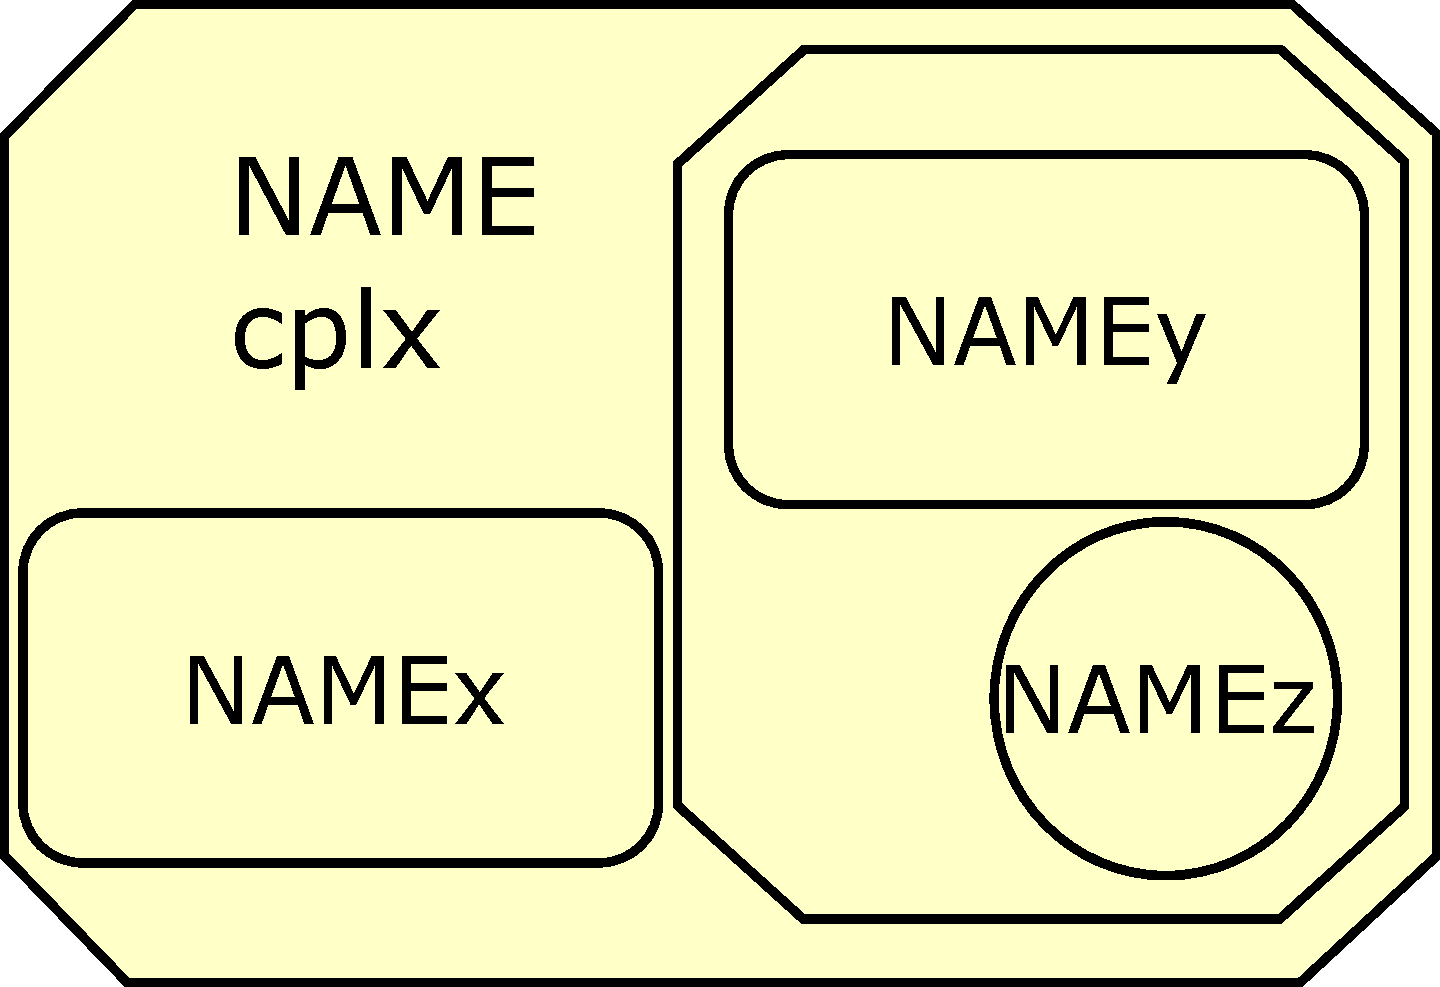
\includegraphics[width = 3.0in]{images/complex}
  \caption{Both these complex glyphs are equivalent. The one on the
    left is described using subunit decorators, the one on the right
    describes the same thing without them.}
  \label{fig:techref:complexSubunits}
\end{figure}

\subsubsection{Changes from Previous Version}

In previous version of the spec the subunits of a \sbgnclass{Complex}
were regarded as an EPN. This however, is incorrect as it implies
there are pools within pools, which breaks one of the fundamental
paradigms of the \PDl. This is corrected in the current version and
subunits are now adornments of the \sbgnclass{Complex}.

\subsection{ProcessNode}\label{sec:techref:PNs}
\label{defn:ProcessNode}

The \sbgnclass{Process} (figure \ref{fig:techref:processumlview}) represents a
process that transforms one or more entity pools into one or more
entity pools, that are identical or different. A process may be used
to represent or summarise more than one known process.

\begin{figure}[htb]
  \centering
  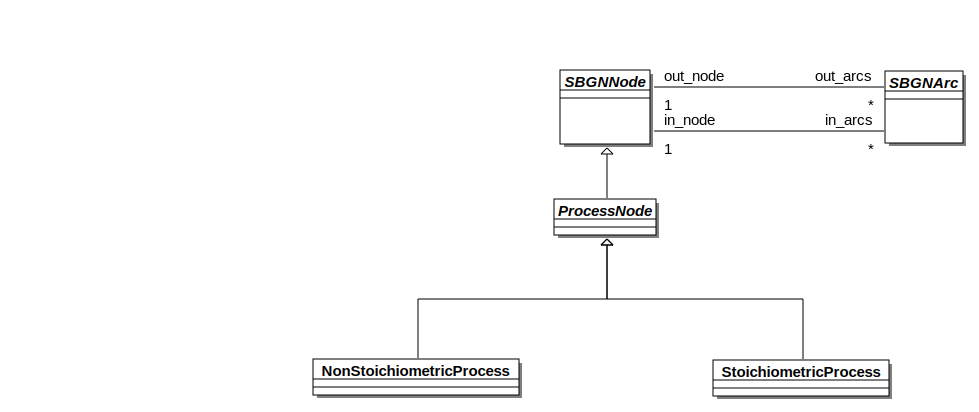
\includegraphics[width = 0.65\textwidth]{images/processumlview}
  \caption{The UML definition of the \sbgnclass{Process} and its
    associated subclasses. Note that the \sbgnclass{Process} extends
    \sbgnclass{SBGNNode} so all its descendants can potentially be
    nodes in a directed graph.}
  \label{fig:techref:processumlview}
\end{figure}


\subsubsection{Generalisation}

\begin{itemize}
\item \classref{SBGNNode}
\end{itemize}

\subsubsection{Attributes}

No additional attributes.

\subsubsection{Associations}

No additional associations.

\subsubsection{Rules and Constraints}

No additional rules and constraints.

\subsubsection{Changes from Previous Version}
\begin{itemize}
\item This was not explicitly defined in the previous version, but
  this version did define a glyph called \glyph{Process}. To avoid
  ambiguity this glyph has now been renamed \glyph{Stoichiometric
    Process} (see section \ref{sec:techref:stoichiometricprocess}).
\item Previous specifications stated that processed could be
  duplicated when all associated EPNs were cloned. This behaviour has
  been changed the current status where all processes are unique in a \PDm.
\end{itemize}

\subsection{NonStoichiometricProcess}
\label{defn:NonStoichiometricProcess}

The \sbgnclass{NonStoichiometricProcess}\query{This has been discussed
  and agreed in past meetings} (figure \ref{fig:techref:nonstoichprocessuml})
is a type of process. It does not necessarily result in a measurable
change of entity pools, nor does it necessarily have a defined start
and end point. In many cases the process is not well defined. This may
because it is not well understood or because the detail is not
important or is being summarised.

\begin{figure}[htb]
  \centering
  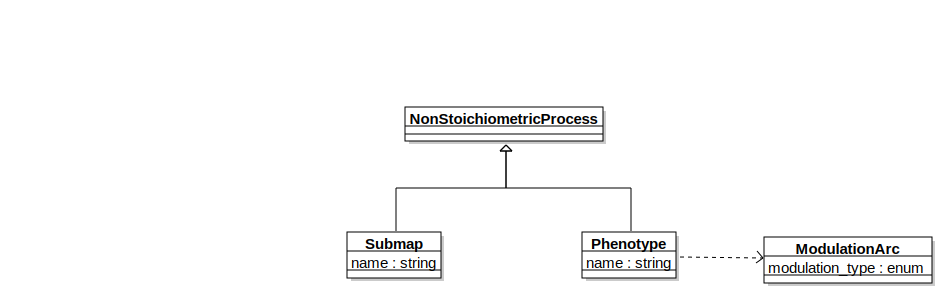
\includegraphics[width = 0.45\textwidth]{images/nonstoichprocessuml}
  \caption{The UML definition of the \sbgnclass{NonStoichiometricProcess} and its
    associated subclasses.}
  \label{fig:techref:nonstoichprocessuml}
\end{figure}

\subsubsection{Generalisation}

\begin{itemize}
\item \classref{ProcessNode}
\end{itemize}

\subsubsection{Attributes}

No additional attributes.

\subsubsection{Associations}

No additional associations.

\subsubsection{Rules and Constraints}

No additional rules and constraints.

\subsubsection{Changes from Previous Version}

Not defined in the previous version.

\subsection{Phenotype}

A biochemical network can generate phenotypes or affect biological
processes.  Such processes can take place at different levels and are
independent of the biochemical network itself.  To represent these
processes in a map, SBGN defines the \sbgnclass{Phenotype} (figure \ref{fig:techref:nonstoichprocessuml}).

\subsubsection{Generalisation}

\begin{itemize}
\item \classref{NonStoichiometricProcess}
\end{itemize}

\subsubsection{Attributes}

\begin{attributes}
  \attitem{name}{string}{R} The name of the phenotype.
\end{attributes}

\subsubsection{Associations}

No additional associations.

\subsubsection{Unique Key}

\begin{logicalkey}
\item \attrib{owning\_map}
\item \attrib{name}
\end{logicalkey}

\subsubsection{Rules and Constraints}

\begin{itemize}
\item The number of \attrib{in\_arcs} must be $>0$.
\item \attrib{in\_arc} can only contain instances of
\classref{ModulationArc} and its subclasses.
\item \attrib{out\_arcs} must be empty.
\end{itemize}

\subsubsection{Notation}

\paragraph{Glyph: \glyph{Phenotype}}
\label{sec:techref:phenotype}

\begin{glyphDescription}

\glyphSboTerm SBO:0000358 ! phenotype

\glyphContainer A \glyph{phenotype} is represented by an elongated
hexagon, as illustrated in \fig{techref:phenotype}.

\glyphLabel A \glyph{phenotype} is identified by a label placed in an
unbordered box containing a string of characters.  The characters can be
distributed on several lines to improve readability, although this is not
mandatory.  The label box must be attached to the center of the
\glyph{phenotype} container.  The label may spill outside of the container.
\end{glyphDescription}

\begin{figure}[htb]
  \centering
  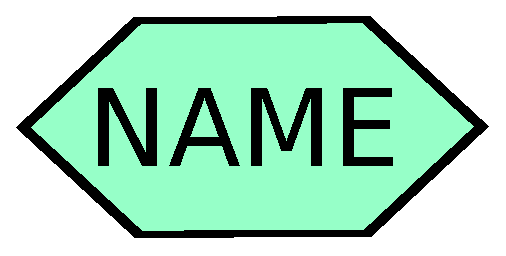
\includegraphics[scale = 0.3]{images/phenotype}
  \caption{The \PD glyph for \glyph{phenotype}.}
  \label{fig:techref:phenotype}
\end{figure}


\subsubsection{Changes from Previous Version}

This definition clarifies that the \sbgnclass{Phenotype} cannot be
cloned as it is now a subclass of \sbgnclass{Process}, which is always
unique.


\subsection{SubmapNode}
\label{sec:techref:submap}\label{defn:SubmapNode}

The \sbgnclass{SubmapNode}\query{This name change has not been
  discussed at the time of writing. The aim is to provide clarity
  between the submap and this glyph.} (figure \ref{fig:techref:submapnodeuml}) is a
placeholder for another process and is used when one wishes to hide
the detail of this process from the \PDm, but make it available to the
reader as a separate related map. The \sbgnclass{Submap} is not
equivalent to an \sbgnclass{OmittedProcess} (section
\ref{sec:techref:omitted}). The \sbgnclass{Submap} allows the detail of
section of the \PDm to be exported to another \PDm and replaced by the
\sbgnclass{SubmapNode}, which acts as a place-holder.  This is
described in section \ref{sec:techref:map} and the semantics of submap linking
is defined in section \ref{sec:techref:submaplinkingsemantics}.

\begin{figure}[htb]
  \centering
  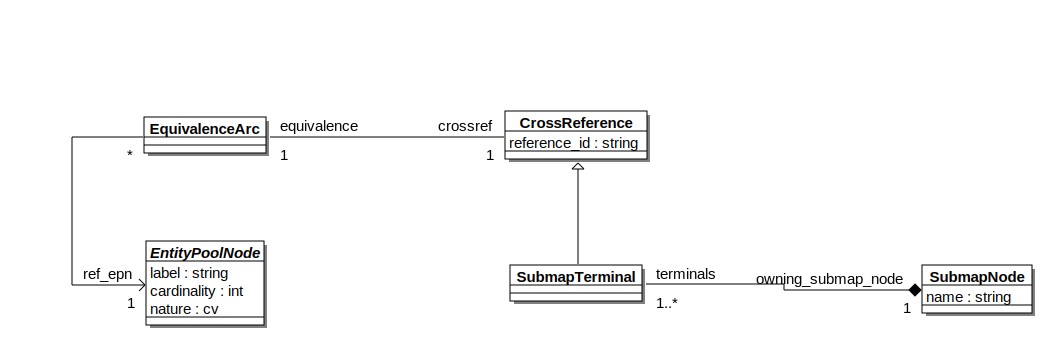
\includegraphics[width = 0.65\textwidth]{images/submapnodeuml}
  \caption{The UML definition of the \sbgnclass{SubmapNode} and its
   relationship to its submap, tags etc.}
  \label{fig:techref:submapnodeuml}
\end{figure}

\subsubsection{Generalisation}

\begin{itemize}
\item \classref{NonStoichiometricProcess}
\end{itemize}

\subsubsection{Attributes}

\begin{attributes}
  \attitem{name}{string}{R} The name of the submap that is being
  summarised. Note that this name ideally will indicate the function
  or the processes that are being summarised.
\end{attributes}

\subsubsection{Associations}

\begin{attributes}
\associtem{terminals}{SubmapTerminal}{1..*} The terminals provide a
reference between the EPNs in the Main Map and those in the submap,
which are identified by a \sbgnclass{Tag}.
\end{attributes}

\subsubsection{Unique Key}

\begin{logicalkey}
  \item \attrib{owning\_map}
  \item \attrib{name}
\end{logicalkey}

\subsubsection{Rules and Constraints}

\begin{itemize}
\item All instances of \classref{SubmapTerminal} held by this class
  must be logically unique.
\item attrib{in\_arcs} and \attrib{out\_arcs} must be empty (\ie
  degree $=0$).
\end{itemize}

\subsubsection{Notation}

\paragraph{Glyph: \glyph{Submap Node}}

\begin{glyphDescription}

\glyphSboTerm SBO:0000395 ! encapsulating process

\glyphContainer The \glyph{submap} is represented as a square box to remind the viewer that it is fundamentally a process.

\glyphLabel The identification of the \glyph{submap} is carried by an unbordered box containing a string of characters.  The characters may be distributed on several lines to improve readability, although this is not mandatory.  The label box has to be attached to the center of the container box.

\end{glyphDescription}


\begin{figure}[htb]
  \centering
  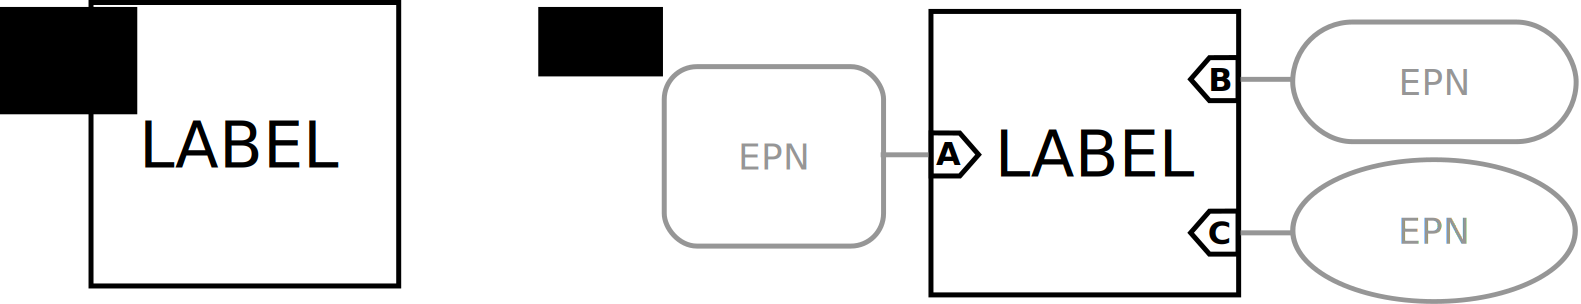
\includegraphics[scale = 0.22]{images/submapglyph}
  \caption{The \PD glyph for \glyph{submap}. (a) the basic glyph
    symbol, without the \glyph{submap terminal} auxiliary units that
    would normally be associated with it. (b) The glyph as it would
    typically be used within a map --- associated with EPN glyphs and
    containing \glyph{submap terminals}.}
  \label{fig:techref:submap}
\end{figure}

\subsubsection{Changes from Previous Version}

This glyph was called \glyph{Submap} in previous version of the \PD
specification. This is confusing when talking about the Submap itself
so this glyph is now referred to as the SubmapNode to distinguish it.

\subsection{LogicalOperator}
\label{sec:techref:logic}
\label{defn:LogicalOperator}

\begin{figure}[htb]
  \centering
  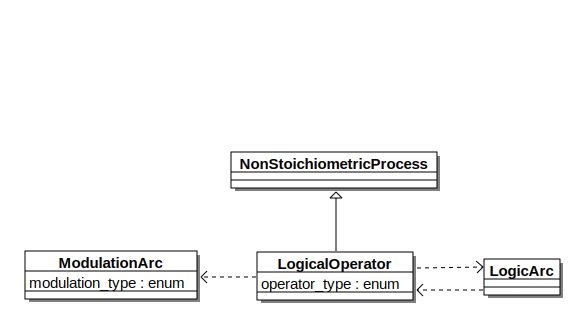
\includegraphics[width = 0.5\textwidth]{images/logicaloperatoruml}
  \caption{The UML definition of the \sbgnclass{LogicalOperator}.}
  \label{fig:techref:logicaloperatoruml}
\end{figure}

 The \sbgnclass{LogicalOperator} (figure \ref{fig:techref:logicaloperatoruml} performs a Boolean operation on one or
more inputs to give a binary output. The input must be a Boolean
value, and are obtained from the \classref{LogicArc} connected to the
\sbgnclass{LogicOperator}. The output a two-value quantity,  0 for False and positive
non-zero for True. This is required because the output of the
\sbgnclass{LogicOperator} must be connected to either a
\sbgnclass{LogicArc} or a \classref{ModulationArc} both of which
require their out node to provide a quality. The behaviour of the
logical operator for each type of \attrib{operator\_type} is shown in
the following table:

\begin{tabular}[t]{c p{12cm}}
\toprule
AND & All inputs must be True for output to be True, otherwise output
is false.\\
OR & At least one input must be True for output to be True. If all
inputs are False then output is False.\\
NOT & Only one input is permitted and the output is the inversion of
the input. Therefore True gives False and False gives True.\\
\bottomrule
\end{tabular}

\subsubsection{Generalisation}

\begin{itemize}
\item \classref{NonStoichiometricProcess}
\end{itemize}

\subsubsection{Attributes}

\begin{attributes}
  \attitem{operator\_type}{enum}{R} The operator type must be one of the
  following enumerations: AND, OR, NOT.
\end{attributes}

\subsubsection{Associations}

No additional associations.

\subsubsection{Rules and Constraints}

\begin{itemize}
\item \attrib{in\_arc} can only contain one or more instances of
  \sbgnclass{LogicArc}.
\item \attrib{out\_arc} can only contain one or more instances of
  \sbgnclass{LogicArc} or \sbgnclass{ModulationArc}.
\item if \attrib{operator\_type} is AND or OR, then \attrib{in\_arc} must
  contain two or more arcs.
\item if \attrib{operator\_type} is NOT then \attrib{in\_arc} must
  contain only one arc.
\item \attrib{out\_arc} can contain only one arc.
\end{itemize}

\subsubsection{Notation}

Three glyphs are used to represent the different operator types. The
glyphs are names after the corresponding type.

\paragraph{Glyph: \glyph{And}}\label{sec:techref:and}

\begin{glyphDescription}
 \glyphSboTerm SBO:0000173 ! and.
 \glyphNode \glyph{And} is represented by a circle carrying the word ``AND''.
\end{glyphDescription}

\begin{figure}[htb]
  \centering
  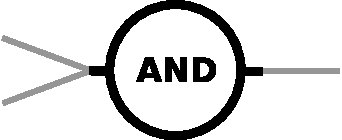
\includegraphics[scale = 0.5]{images/and}
  \caption{The \PD glyph for \glyph{and}. Only two inputs are represented, but more would be allowed.}
  \label{fig:techref:and}
\end{figure}


\paragraph{Glyph: \glyph{Or}}\label{sec:techref:or}

\begin{glyphDescription}
 \glyphSboTerm SBO:0000174 ! or.
 \glyphNode \glyph{Or} is represented by a circle carrying the word ``OR''.
 \end{glyphDescription}

\begin{figure}[htb]
  \centering
  \includegraphics[scale = 0.5]{images/or}
  \caption{The \PD glyph for \glyph{or}. Only two inputs are represented, but more would be allowed.}
  \label{fig:techref:or}
\end{figure}


\paragraph{Glyph: \glyph{Not}}\label{sec:techref:not}

\begin{glyphDescription}
 \glyphSboTerm SBO:0000238 ! not.
 \glyphNode \glyph{Not} is represented by a circle carrying the word ``NOT''.
 \end{glyphDescription}

\begin{figure}[htb]
  \centering
  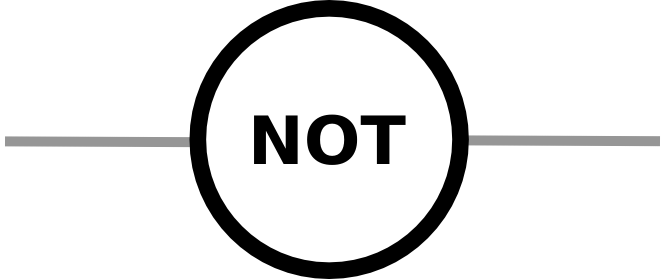
\includegraphics[scale = 0.5]{images/not}
  \caption{The \PD glyph for \glyph{not}.}
  \label{fig:techref:not}
\end{figure}

\subsubsection{Changes from Previous Version}

Although the \sbgnclass{LogicOperator} was not explicitly defined in
the previous version the semantics and glyphs are unchanged.


\subsection{StoichiometricProcess}
\label{defn:StoichiometricProcess}\label{sec:techref:stoichiometricprocess}

\begin{figure}[htb]
  \centering
  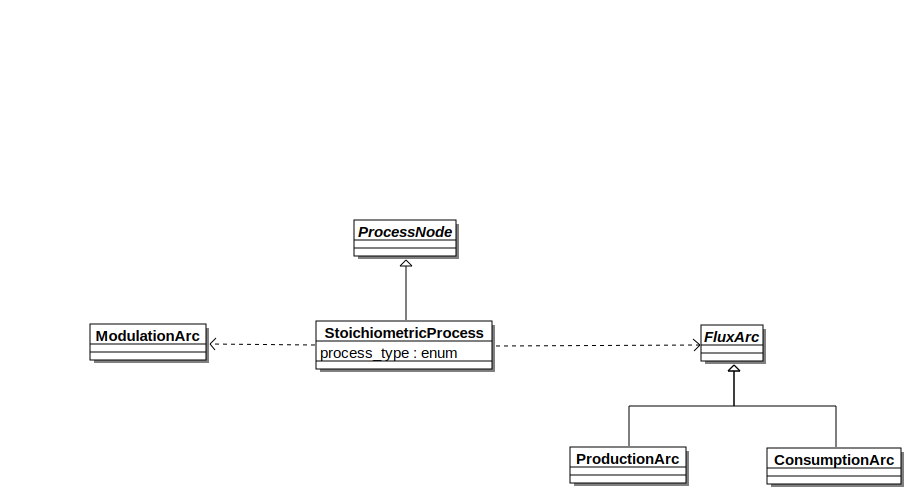
\includegraphics[width = 0.45\textwidth]{images/stoichprocessuml}
  \caption{The UML definition of the
    \sbgnclass{StiochiometricProcess}. The class interacts with
    subclasses of \sbgnclass{FluxArc} and \sbgnclass{ModulationArc}.}
  \label{fig:techref:stoichprocessuml}
\end{figure}

A stoichiometric process\query{New concept, but discussed in previous
  meetings. The semantics of the process being stoichiometrically
  balanced has not been discussed in detail for the stoichiometric
  process, and this is the subject of a tracker query. The spec
  previously stated that the process should be balanced and this is
  therefore consistent with that.} produces a measurable change in the
quantities of entity pools consumed and produced. This might imply
modification of covalent bonds (conversion), modification of the
relative position of constituents (conformational process) or movement
from one compartment to another (translocation). Such a process will
have a basal rate at which this change occurs, which can be affected
positively or negatively by the other entity pools, which 'modulate'
the process. Examples of this include stimulation, inhibition and
catalysis. In an irreversible process the entity pools interacting
with it can be grouped into inputs and outputs. However, a
stoichiometric process can also be reversible and so for convenience
we refer to these groupings as the ``left-hand-side'' (LHS) and
``right-hand-side'' (RHS) of the process\footnote{Note this
  designation is purely for grouping and is used even then the sides
  of the reaction are above and below the process.}  (figure
\ref{fig:techref:process-sidedness}).

\begin{figure}[htb]
  \centering
  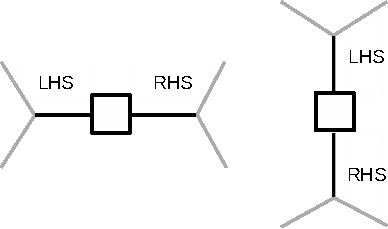
\includegraphics[scale = 0.4]{images/process_sidedness}
  \caption{An illustration of the ``sidedness'' of a process. The designation of LHS and RHS is essentially arbitrary.}
  \label{fig:techref:process-sidedness}
\end{figure}

In the \PDl this is represented by the
\sbgnclass{StoichiometricProcess} (figure \ref{fig:techref:stoichprocessuml}). It
can be one of several different types, which indicate the amount that
is known about the process or in some cases the nature of the process,
for example association and dissociation. The permitted values for
\attrib{process\_type} are described in the following table:

\begin{tabular}[c]{l p{10cm}}
\\\toprule
generic & A generic stoichiometric process that transforms a set of entity pools into another set of entity pools.\\
omitted & Omitted processes are processes that are known to exist, but are omitted from the map for the sake of clarity or parsimony. A single \glyph{omitted process} can represent any number of actual processes. The \glyph{omitted process} is different from a \glyph{submap}. While a \glyph{submap} references to an explicit content, that is hidden in the main map, the \glyph{omitted process} does not ``hide'' anything within the context of the map, and cannot be ``unfolded''.\\
uncertain & Uncertain processes are processes that may not exist. A single \glyph{uncertain process} can represent any number of actual processes.\\
association & The association between one or more \glyph{EPNs} represents the non-covalent binding of the biological objects represented by those \glyph{EPNs} into a larger complex.\\
dissociation & The dissociation of an \glyph{EPN} into one or more \glyph{EPNs} represents the rupture of a non-covalent binding between the biological entities represented by those \glyph{EPNs}.\\
\bottomrule\\
\end{tabular}\\

Since this process is stoichiometric the relative quantities of the
entity pools participating the process must be specified. For this
reason the \classref{FluxArc} has an \attrib{stoichiometry} attribute
and each \classref{EntityPoolNode} has a cardinality, which should be
balanced in a valid \PDm. This is especially important where there is
potential ambiguity in the stoichiometry of the process (figure \ref{fig:techref:prod-card}).



\begin{figure}[htb]
  \centering
  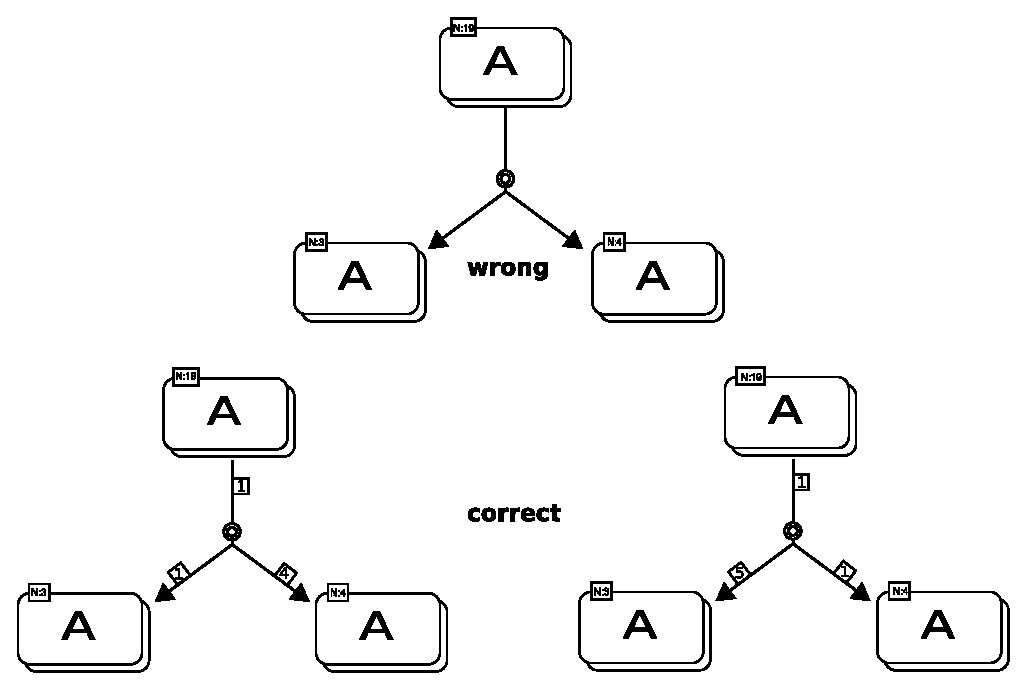
\includegraphics[width=0.6\textwidth]{examples/stoichEx1}
  \caption{The figure illustrates why for the stoichiometry label is
    required to clarify potentially ambiguous stoichiometry. In the
    top example there is more than one possible solution, which can
    only be made clear using the stoichiometry labels in the bottom examples.}
  \label{fig:techref:prod-card}
\end{figure}



\label{sec:techref: semantics reversible procs}

A stoichiometric process is deemed to be reversible its
\attrib{in\_arcs} are \sbgnclass{FluxArc}s of type `reversible' (see
figure \ref{fig:techref:process-reversibility}).  Semantically, this permits a
reversible flow of entities through the process.  Modulation of a
reversible process affects the rate of flux through the process, but
does not directly affect the direction of that flow.

\begin{figure}[htb]
  \centering
  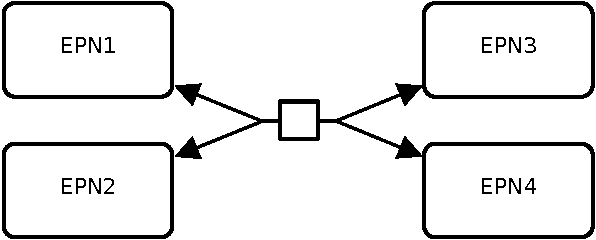
\includegraphics[scale = 0.4]{images/reversible_process}
  \caption{A valid reversible process. A process is reversible if its LHS and RHS contain only \glyph{production} arcs.}
  \label{fig:techref:process-reversibility}
\end{figure}

\subsubsection{Generalisation}

\begin{itemize}
\item \classref{ProcessNode}
\end{itemize}

\subsubsection{Attributes}

\begin{attributes}
  \attitem{process\_type}{enum}{R} This must be one of the following
  enumerations: generic, omitted, uncertain, association, dissociation.
\end{attributes}

\subsubsection{Associations}

No additional associations.

\subsubsection{Rules and Constraints}

\paragraph{General}

\begin{itemize}
\item The \attrib{in\_arc} must contain one or more
  \sbgnclass{FluxArc}s containing the same \attrib{flux\_type} value.
\item The \attrib{in\_arc} may only contains \sbgnclass{FluxArc}
  instances with a \attrib{flux\_type} of `consumption', or `reversible'.
\item In addition the \attrib{in\_arc} may contain zero, one or more
  instances of \sbgnclass{ModulationArc}.
\item The \attrib{out\_arc} must contain one or more
 instances of \sbgnclass{FluxArc} with a \attrib{flux\_type} or `production'.
\item If \attrib{in\_arcs}  contains one or more \sbgnclass{FluxArc}s
  of type `reversible' this process reversible.
\item The \sbgnclass{EntityPoolNode}s that make up the LHS of the
  process should be consistent with the RHS, i.e.\, the process should
 be stoichiometrically balanced.\query{Tracker issue 329060. If the
   process is stoichiometric this must make sense. The previous spec
   states this so this is consistent with it.}
\item If at least one \sbgnclass{FluxArc} associated with a
  \sbgnclass{StoichiometricProcess} displays its stoichiometry via a
  \glyph{stoichiometry label} then all must.\query{Take from previous
    spec, but that said if one displays stoichiometry in a map which
    is too restrictive.}
\item If more than one set of stoichiometries can be applied to the
  flux arcs of the process then the stoichiometry of the flux arcs
  must be displayed.
\end{itemize}


\paragraph{Association}

These rules apply if the \attrib{process\_type} is `association'.

\begin{itemize}
\item The process must be irreversible.
\item There can only be one `production' \sbgnclass{FluxArc}, with
  \attrib{stoichiometry} $= 1$.
\item If a \sbgnclass{Complex} is on the RHS of the association then
  there must be at least 2 EPNS on the LHS.\glyph{Is this too
    restrictive? It prevents multimers being represented as a complex
    of 2 identical subunits. It is taken from v1.0 of the spec and got lost in
    later versions.}
\end{itemize}

\paragraph{Dissociation}

These rules apply if the \attrib{process\_type} is `dissociation'.

\begin{itemize}
\item The process must be irreversible.
\item There can only be one `consumption \sbgnclass{FluxArc}, with
  \attrib{stoichiometry} $= 1$.
\item If a \sbgnclass{Complex} is on the LHS of the dissociation then
  there must be at least 2 EPNS on the RHS.\glyph{see comment in
    association rules}.
\end{itemize}

\subsubsection{Notation}

\paragraph{Glyph: \glyph{Process}}
\label{sec:techref:process}

\begin{glyphDescription}

\glyphSboTerm SBO:0000375 ! process

\glyphNode A process is represented by a square box linked to two
connectors: small arcs attached to the centers of opposite sides and
referred to here as `lugs'\query{The term lugs is used in
  discussion. We haven't discussed this in detail or at least come to
  a consensus on it. In particular does the lug need to be
  perpendicular to the process and does it need to be a straight line?
  How should it be used when the arc connecting to it is curved.}. The
flux arcs arcs are linked to the ends of the lugs as shown in figure
\ref{fig:techref:process}. The lug's purpose is to 'gather' the flux arcs
together before meeting the process node proper and in doing so they
emphasis the 'sides' of the reaction. Therefore the lug must have a
visually appreciable length\query{Undefined previously, but if we
  define it then it should be visible.} and must be placed on opposite sides
of the process square. The modulatory arcs (section
\ref{sec:techref:modulation}) point to the other two sides of the box.

\end{glyphDescription}

\begin{figure}[htb]
  \centering
  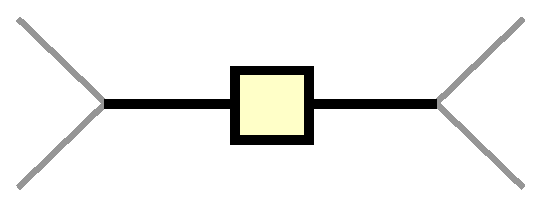
\includegraphics[scale = 0.4]{images/process}
  \caption{The \PD glyph for \glyph{process}.}
  \label{fig:techref:process}
\end{figure}


The example in \fig{techref:trans-phos} illustrates the use of a \glyph{process} node to represent the phosphorylation of a protein in a \PD.

\begin{figure}[htb]
  \centering
  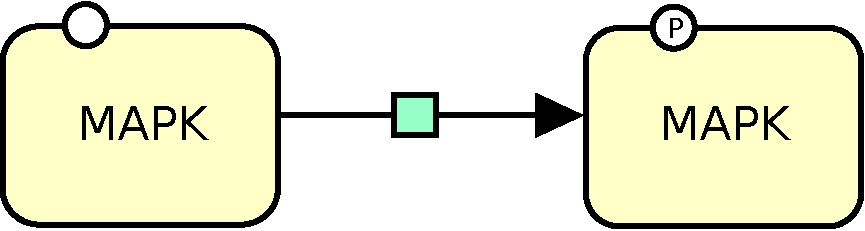
\includegraphics[scale = 0.3]{examples/process-phosphorylation}
  \caption{Phosphorylation of the protein MAP kinase.}
  \label{fig:techref:trans-phos}
\end{figure}

The example in \fig{techref:trans-react} illustrates the use of a \glyph{process} node to represent a reaction between two reactants that generates three products.

\begin{figure}[htb]
  \centering
  \includegraphics[scale = 0.3]{examples/process-reaction}
  \caption{Reaction between ATP and fructose-6-phosphate to produce fructose-1,6-biphosphate, ADP and a proton.}
  \label{fig:techref:trans-react}
\end{figure}

The example in \fig{techref:trans-trans} illustrates the use of a \glyph{process} node to represent a translocation. The large round-cornered rectangle represents a compartment border (see \sect{techref:compartment}).

\begin{figure}[htb]
  \centering
  \includegraphics[scale = 0.3]{examples/process-translocation}
  \caption{Translocation of calcium ion out of the endoplasmic reticulum. Note that the \glyph{process} does not have to be located on the boundary of the \glyph{compartment}. A \glyph{process} is not attached to any \glyph{compartment}.}
  \label{fig:techref:trans-trans}
\end{figure}

The example in \fig{techref:trans-reverse} illustrates the use of a \glyph{process} node to represent the reversible opening and closing of an ionic channel in a \PD.

\begin{figure}[htb]
  \centering
  \includegraphics[scale = 0.3]{examples/process-reversible}
  \caption{Reversible opening and closing of an ionic channel.}
  \label{fig:techref:trans-reverse}
\end{figure}

When such a reversible process is asymmetrically modulated, it must be represented by two different processes in a \PD.  \fig{techref:trans-mod} illustrates the use of two \glyph{process} nodes to represent the reversible activation of a G-protein coupled receptor.  In the absence of any effector, an equilibrium exists between the inactive and active forms.  The agonist stabilises the active form, while the inverse agonist stabilises the inactive form.

\begin{figure}[htb]
  \centering
  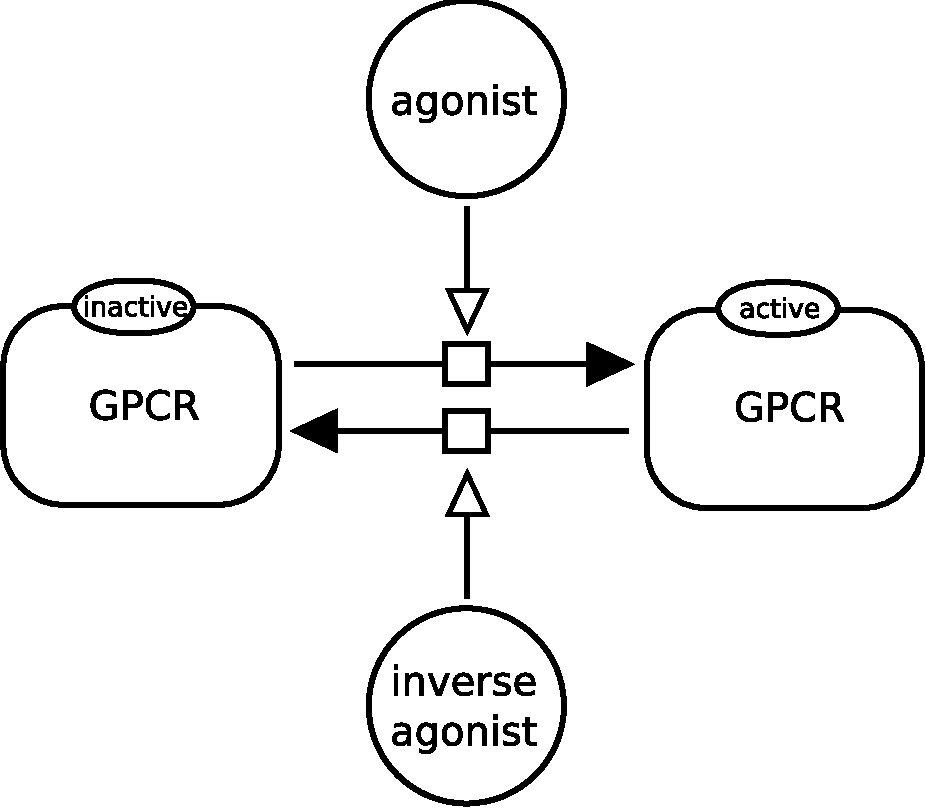
\includegraphics[scale = 0.3]{examples/process-modulated}
  \caption{The reversible activation of a G-protein coupled receptor.}
  \label{fig:techref:trans-mod}
\end{figure}

The example in \fig{techref:trans-dim} presents the conversion of two galactoses into a lactose.  Galactoses are represented by only one \glyph{simple chemical}, the cardinality being carried by the \glyph{consumption} arc.

\begin{figure}[htb]
  \centering
  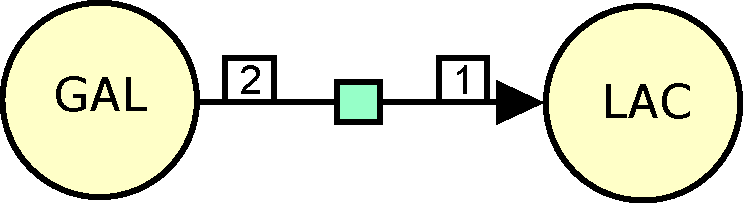
\includegraphics[scale = 0.3]{examples/process-dimerisation}
  \caption{Conversion of two galactoses into a lactose.}
  \label{fig:techref:trans-dim}
\end{figure}


%%%%%%%%%%%%%%%%%%%%%%%%%%%%%%%%%%%%%%%%%%%%%%%%%%%%%%%%%%%%%%%%%%%%%%
%%                     Omitted Process
%%%%%%%%%%%%%%%%%%%%%%%%%%%%%%%%%%%%%%%%%%%%%%%%%%%%%%%%%%%%%%%%%%%%%%

\paragraph{Glyph: \glyph{Omitted process}}\label{sec:techref:omitted}


\begin{glyphDescription}
 \glyphSboTerm SBO:0000397 - omitted process.

 \glyphNode An \glyph{omitted process} is represented by a \glyph{process} in which the square box contains a two parallel slanted lines oriented northwest-to-southeast and separated by an empty space.
 \end{glyphDescription}

\begin{figure}[htb]
  \centering
  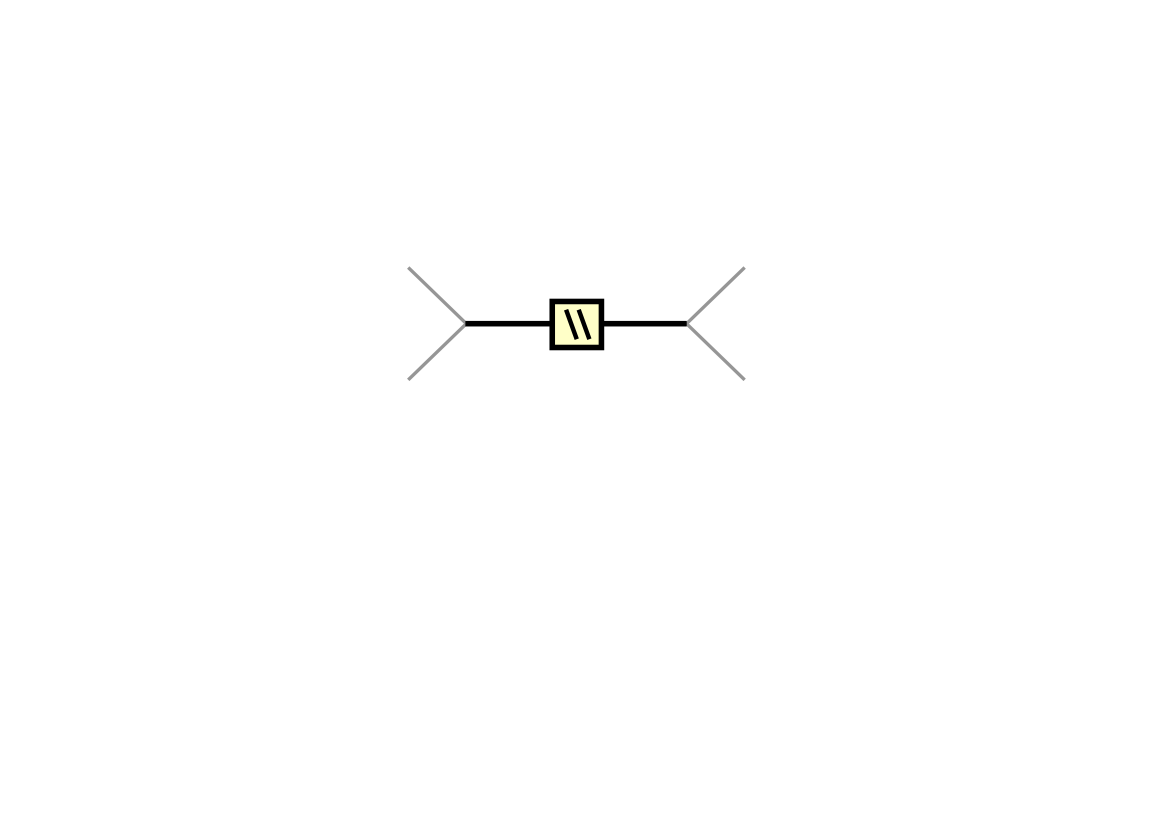
\includegraphics[scale = 0.5]{images/omitted}
  \caption{The \PD glyph for \glyph{omitted process}.}
  \label{fig:techref:omitted}
\end{figure}


%%%%%%%%%%%%%%%%%%%%%%%%%%%%%%%%%%%%%%%%%%%%%%%%%%%%%%%%%%%%%%%%%%%%%%
%%                     Uncertain Process
%%%%%%%%%%%%%%%%%%%%%%%%%%%%%%%%%%%%%%%%%%%%%%%%%%%%%%%%%%%%%%%%%%%%%%

\paragraph{Glyph: \glyph{Uncertain process}}\label{sec:techref:uncertain}

\begin{glyphDescription}
 \glyphSboTerm SBO:0000396 ! uncertain process.
 \glyphNode An \glyph{uncertain process} is represented by a \glyph{process} which square box contains a question mark.
 \end{glyphDescription}

\begin{figure}[htb]
  \centering
  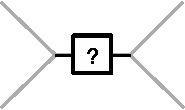
\includegraphics[scale = 0.5]{images/uncertain}
  \caption{The \PD glyph for an \glyph{uncertain process}.}
  \label{fig:techref:uncertain}
\end{figure}


%%%%%%%%%%%%%%%%%%%%%%%%%%%%%%%%%%%%%%%%%%%%%%%%%%%%%%%%%%%%%%%%%%%%%%
%%                     Association
%%%%%%%%%%%%%%%%%%%%%%%%%%%%%%%%%%%%%%%%%%%%%%%%%%%%%%%%%%%%%%%%%%%%%%

\paragraph{Glyph: \glyph{Association}}\label{sec:techref:association}


\begin{glyphDescription}
 \glyphSboTerm SBO:0000177 ! non-covalent binding.
 \glyphNode An \glyph{association} between several entities is represented by a filled disc linked to two connectors, small arcs attached on point separated by 180 degrees. The consumption (\sect{techref:consumption}) and production (\sect{techref:production}) arcs are linked to the extremities of those connectors.
 \end{glyphDescription}

\begin{figure}[htb]
  \centering
  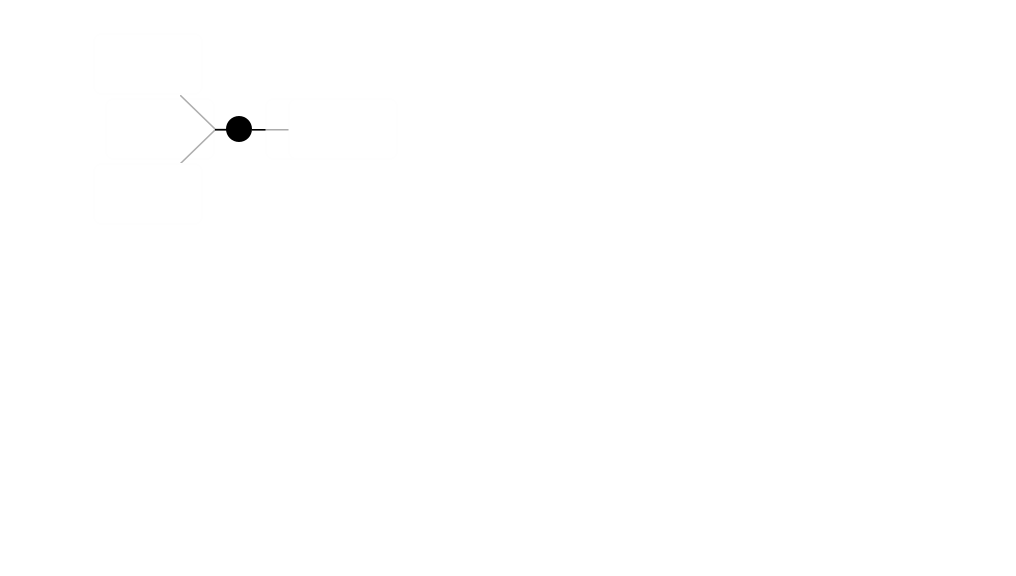
\includegraphics[scale = 0.5]{images/association}
  \caption{The \PD glyph for \glyph{association}.}
  \label{fig:techref:association}
\end{figure}

The example in \fig{techref:assoc-cyclin} illustrates the association of cyclin and CDC2 kinase into the Maturation Promoting Factor.

\begin{figure}[htb]
  \centering
  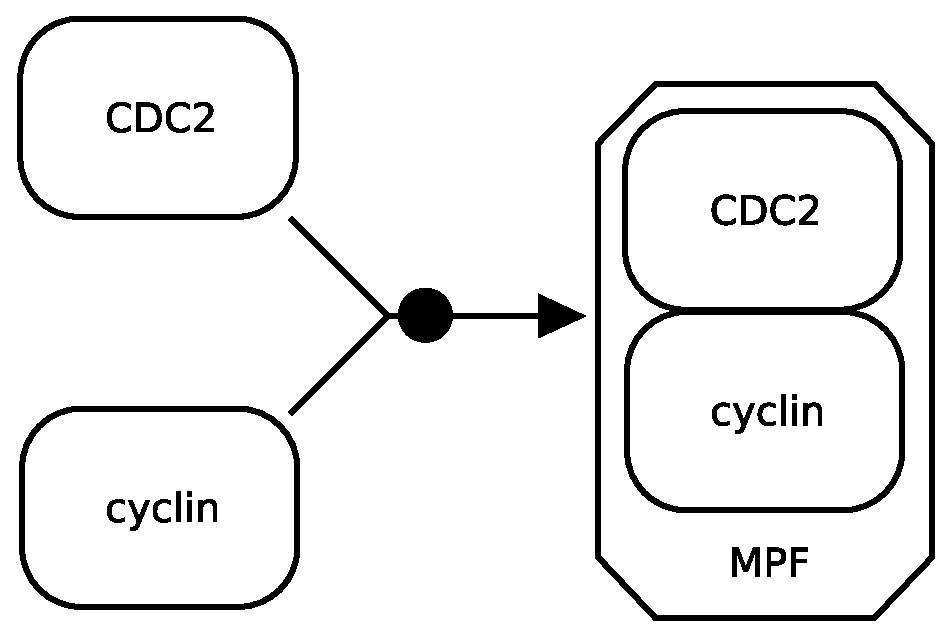
\includegraphics[scale = 0.3]{examples/association-MPF}
  \caption{Association of cyclin and CDC2 kinase into the Maturation Promoting Factor.}
  \label{fig:techref:assoc-cyclin}
\end{figure}

\fig{techref:assoc-unamed} gives an example illustrating the association of a pentameric macromolecule (a nicotinic acetylcholine receptor) with a simple chemical (the local anesthetic chlorpromazin) in an unnamed complex.

\begin{figure}[htb]
  \centering
  \includegraphics[scale = 0.3]{examples/association-unamed}
  \caption{The association of a pentameric macromolecule with a simple chemical in an unnamed complex.}
  \label{fig:techref:assoc-unamed}
\end{figure}

% An association does not necessarily result in the formation of a
% \glyph{complex}; it can also produce a multimer, or a
% \glyph{macromolecule} (although the latter case is semantically
% borderline) \query{This is \textbf{wrong} and should be removed. It
%   hould be handled by a process}.  \ref{fig:techref:assoc-multi} gives an example of this, using the formation of hemoglobin.

% \begin{figure}[htb]
%   \centering
%   \includegraphics[scale = 0.3]{examples/association-multimerisation}
%   \caption{Formation of hemoglobin.}
%   \label{fig:techref:assoc-multi}
% \end{figure}

\paragraph{Glyph: \glyph{Dissociation}}\label{sec:techref:dissociation}

\begin{glyphDescription}
 \glyphSboTerm SBO:0000180 ! dissociation.
 \glyphNode A \glyph{dissociation} between several entities is represented by two concentric circles. A simple empty disc could be, in some cases, confused with the \glyph{catalysis} (section \sect{techref:catalysis}). Moreover, the existence of two circles reminds the dissociation, by contrast with the filled disc of the \glyph{association} (\sect{techref:association}).
 \end{glyphDescription}


\begin{figure}[htb]
  \centering
  \includegraphics[scale = 0.5]{images/dissociation}
  \caption{The \PD glyph for \glyph{dissociation}.}
  \label{fig:techref:dissociation}
\end{figure}

The example in \fig{techref:dissoc-ribo} illustrates the dissociation of the small and large ribosomal subunits from a messenger RNA.

\begin{figure}[htb]
  \centering
  \includegraphics[scale = 0.3]{examples/dissociation-ribosome}
  \caption{Dissociation of the small and large ribosomal subunits from a messenger RNA.}
  \label{fig:techref:dissoc-ribo}
\end{figure}

\subsubsection{Changes from Previous Version}

Although the \sbgnclass{NonStoichiometricProcess} was not explicitly defined in
the previous version the semantics and glyphs are unchanged.

\subsection{Compartment}
\label{sec:techrefcompartment}
\label{defn:Compartment}

\begin{figure}[htb]
  \centering
  \includegraphics[width = 0.5\textwidth]{images/compartmentuml}
  \caption{The UML definition of the \sbgnclass{Compartment} showing
    how it containment of \sbgnclass{EntityPoolNode}.}
  \label{fig:techref:compartmentuml}
\end{figure}

The \sbgnclass{Compartment} is a logical or physical structure that
contains entity pool nodes. An \classref{EntityPoolNode} can only
belong to one compartment. Therefore, the ``same'' biochemical species
located in two different compartments are in fact two different pools.


\subsubsection{Generalisation}

\begin{itemize}
\item \classref{SBGNGlyph}
\end{itemize}

\subsubsection{Attributes}

\begin{attributes}
  \attitem{name}{string}{R} The name of the compartment.
  \attitem{natures}{cv}{*} A set of controlled vocabularies\query{This
 reconciles the use of the Unit of Information to represent the nature
of an EPN by using to present similar information for the
compartment. This is consistent with previous usage, but not with the
usage of the UofI for annotation.} that describes
  a characteristic of the compartment. Zero, one or more values may be
  set, but each one must belong to a different controlled vocabulary.
\end{attributes}

\subsubsection{Associations}

\begin{attributes}
  \associtem{epns}{EntityPoolNode}{*} The
  \sbgnclass{EntityPoolNode}s contained by this compartment.
\end{attributes}

\subsubsection{Unique Key}

\begin{logicalkey}
  \item \attrib{owning\_map}
  \item \attrib{name}
\end{logicalkey}

\subsubsection{Rules and Constraints}

\begin{itemize}
\item \attrib{name} must not be used by another instance of
  \sbgnclass{Compartment} contained by the same instance of
  \sbgnclass{Map}.
\item \attrib{epns} must contain a unique set of
  \sbgnclass{EntityPoolNodes}. See section \ref{sec:techref:epnuniqueness} for
  the definition of \sbgnclass{EntityPoolNode} uniqueness.
\end{itemize}

\subsubsection{Notation}

\paragraph{Glyph: \glyph{Compartment}}\label{sec:techref:compartment}

\begin{glyphDescription}

\glyphSboTerm  SBO:0000290 ! physical compartment

\glyphContainer A compartment is represented by a surface enclosed in a continuous border or located between continuous borders. These borders should be noticeably thicker than the borders of the EPNs. A compartment can take \textbf{any} geometry. A compartment must always be entirely enclosed.

\glyphLabel The identification of the compartment is carried by an unbordered box containing a string of characters. The characters can be distributed on several lines to improve readability, although this is not mandatory. The label box can be attached anywhere in the container box. Note that the label can spill-over from the container box.

\end{glyphDescription}

\begin{figure}[htb]
  \centering
  \includegraphics[scale = 0.3]{images/compartment}
  \caption{The \PD glyph for \glyph{compartment}.}
  \label{fig:techref:compartment}
\end{figure}


To allow more aesthetically pleasing and understandable maps, compartments are allowed to overlap each other visually, but it must be kept in mind that this does not mean the top compartment contains part of the bottom compartment.  \fig{techref:overlap} shows two semantically equivalent placement of compartments:

\begin{figure}[htb]
  \centering
  \includegraphics[scale = 0.4]{examples/compartment_overlapping}
  \caption{Overlapped compartments are permitted, but the overlap does not imply containment.}
  \label{fig:techref:overlap}
\end{figure}

Overlapped (hidden) part of the compartment should not contain any object which could be covered by an overlapping compartment.  \fig{techref:overlap-bad} illustrates the problem using an incorrect map.

\begin{figure}[htb]
  \centering
  \includegraphics[scale = 0.45]{examples/compartment_overlapping_wrong}
  \caption{Example of an \textbf{incorrect} map.  Overlapped compartments must not obscure other objects.}
  \label{fig:techref:overlap-bad}
\end{figure}

% It is important to note that a compartment never contains another compartment, but may surround it.  A key aspect of correctly drawing two ``adjacent'' compartments is that they are not separated by one line, but by \textbf{two} lines.  \fig{techref:two-comp} provides an example of this in which a cell is shown made up of a nucleus surrounded by the cytoplasm.

% \begin{figure}[htb]
%   \centering
%   \includegraphics[scale = 0.4]{examples/compartment-cell}
%  \includegraphics[scale = 0.4]{examples/compartment-cell-wrong}
%   \caption{Compartments can surround other compartments; in that case, both of the compartment's borders must still be shown, with the result that the separation is drawn as two lines. The left example is correct, with twoo disjoint compartments representing the ``cytoplasm'' and the ``nucleus''. The right example is incorrect. Indeed the compartments ``cell'' and ``nucleus'' would be disjoint, the latter only overlapping the former. As a result, the volume of the nucleus is duplicated.}
%   \label{fig:techref:two-comp}
% \end{figure}

% The example diagram in \fig{techref:three-comp} represents three adjacent compartments.  Two of the compartments carry units of information.  Notice that these units of information do not overlap multiple membrane boundaries.

% \begin{figure}[htb]
%   \centering
%   \includegraphics[scale = 0.4]{examples/compartment-3comp}
%   \caption{Illustration of units of information and surrounding compartments.}
%   \label{fig:techref:three-comp}
% \end{figure}

\subsubsection{Changes from Previous Version}

The use \sbgnclass{Compartment} has a set of natures, which previously
were less well specified and handled as notation provided by the
\glyph{unit of information}.  In some cases, where the CVs used are
not distinct or if the \glyph{unit of information} contains arbitrary
text as annotation then maps containing these features will be invalid
according to the current specification.

\subsection{AttributeValue}
\label{defn:AttributeValue}

\begin{figure}[htb]
  \centering
  \includegraphics[width = 0.5\textwidth]{images/attributevalueuml}
  \caption{The UML definition of the \sbgnclass{AttributeValue} and
    its usage by other classes.}
  \label{fig:techref:attributevalueuml}
\end{figure}

The \sbgnclass{AttributeValue}\query{A new concept, that modifies the
  behaviour of the Unit of Information in previous versions with the
  need to use it to present the nature and cardinality of an EPN. The
  glyph retains its original name, but the class has been names to
  reflect it purpose.} is used to present the values of certain
attributes held by other SBGN elements. It is typically contained and
owned by the class containing the attribute (or its descendants). It
contains two values, one is a \attrib{code} to indicate the attribute
that is defined and the other is the\attrib{ value} itself. The
\attrib{code} and the presentation format of the \attrib{value} are
defined by the SBGN element that contains the
\sbgnclass{AttributeValue}, currently \classref{Compartment},
\classref{EntityPoolNode}, and \classref{Subunit}.


\subsubsection{Generalisation}

\begin{itemize}
\item \classref{AuxiliaryUnit}
\end{itemize}

\subsubsection{Attributes}

\begin{attributes}
  \attitem{code}{string}{R} The code indicating the attribute that is
  being presented.
  \attitem{value}{object}{R} The value of the attribute. The format of
  the value is determined by the class holding the attribute.
\end{attributes}

\subsubsection{Associations}

No additional associations.

\subsubsection{Rules and Constraints}

No additional rules and constraints.

\subsubsection{Notation}

For historical reasons the \sbgnclass{AttributeValue} is represented
graphically by the glyph \glyph{Unit of Information}.

\paragraph{Glyph: \glyph{Unit of information}}
\label{sec:techref:unitInfo}

When representing biological entities, it is often necessary to convey
some abstract information about the entity's function that cannot (or
does not need to) be easily related to its structure.  The \glyph{unit
  of information} is a decoration that can be used in this situation
to add information to a glyph.  Some example uses include:
characterizing a logical part of an entity such as a functional domain
(a binding domain, a catalytic site, a promoter, etc.), or the
information encoded in the entity (an exon, an open reading frame,
etc.).  A \glyph{unit of information} can also convey information
about the physical environment, or the specific type of biological
entity it is decorating.

\begin{glyphDescription}

\glyphSboTerm Not applicable.

\glyphContainer A unit of information is represented by a rectangle.  The long side of the rectangle should be oriented parallel to the border of the \glyph{EPN} being annotated by the \glyph{unit of information}. The center of the bounding box of a \glyph{state of information} should be located on the mid-line of the border of the \glyph{EPN}.

\glyphLabel A \glyph{unit of information} is identified by a label placed in an unbordered box containing a string of characters.  The characters can be distributed on several lines to improve readability, although this is not mandatory.  The label box must be attached to the center of the container.  The label may spill outside of the container.


\end{glyphDescription}

\begin{figure}[htb]
  \centering
  \includegraphics[scale = 0.3]{images/unitInformation}
  \caption{The \PD glyph for \glyph{unit of information}. (a) The
    glyph. (b) An example of its usage with a \glyph{macromolecule}.}
  \label{fig:techref:unitInfo}
\end{figure}


\subsubsection{Changes from Previous Version}

There was no definition of the \sbgnclass{AttributeValue} in the
previous version of this specification. However, the \glyph{Unit of
  Information} did exist although its semantics have been changed. It
no longer can hold arbitrary annotation but must display an attribute
value and observe the constraints set out by the definition of the
class owning the attribute.

Since the use of the \glyph{Unit of Information} has been deprecated,
it is recommended that \classref{Annotation} and the
\glyph{Annotation} glyph is used instead.

\subsection{StateVariable}
\label{defn:StateVariable}

Many biological entities such as molecules can exist in different
\emph{states}, meaning different physical or informational
configurations.  These states can arise for a variety of reasons.  For
example, macromolecules can be subject to post-synthesis
modifications, wherein residues of the macromolecules (amino acids,
nucleosides, or glucid residues) are modified through covalent linkage
to other chemicals.  Other examples of states are alternative
conformations as in the closed/open/desensitized conformations of a
transmembrane channel, and the active/inactive forms of an enzyme.

In the \PDl these states are defined by the
\sbgnclass{StateVariableDefinition}s associated with the
\sbgnclass{EntityType}, but the specific values of the variables are
define by the \sbgnclass{StateVariable} (figure
\ref{fig:techref:statevariableviewuml}) associated with the
\sbgnclass{EntityPoolNode}. For every
\sbgnclass{StateVariableDefinition} associated with an
\sbgnclass{EntityType} there should be a corresponding
\sbgnclass{StateVariable} associated with the instance of
\sbgnclass{EntityPoolNode} using that type. This enforces one of the
fundamental rules of the language that once a state variable has been
displayed for a given entity type, then it must always be displayed.

\begin{figure}[htb]
  \centering
  \includegraphics[width = 0.5\textwidth]{images/statevariableviewuml}
  \caption{The UML definition of the \sbgnclass{StateVariable} showing
    its relationship to \sbgnclass{StatefulEPN} and \sbgnclass{StateVariableDefinition}.}
  \label{fig:techref:statevariableviewuml}
\end{figure}

\subsubsection{Generalisation}

\begin{itemize}
\item \classref{AuxiliaryUnit}
\end{itemize}

\subsubsection{Attributes}

\begin{attributes}
  \attitem{value}{string}{R} The value of the state variable. This is
  optional, but cannot be an empty string, should start with a
  non-space character and end with a non-space character. It should
  also not include the `@' character\query{Not specified is previous
    spec, but seems essential if we are to avoid ambiguity.}.
\end{attributes}

\subsubsection{Associations}

\begin{attributes}
  \associtem{owning\_epn}{StatefulEPN}{1}  The stateful EPN that owns
  the state variable.
  \associtem{definition}{StateVariableDefinition}{1} The definition of
  this state variable\query{New concept. It aims to ensure that all
    state variables are defined in all EPNS of the same
    type.}.
\end{attributes}

\subsubsection{Rules and Constraints}

No additional rules and constraints.

\subsubsection{Notation}


\paragraph{Glyph: \glyph{State variable}}
\label{sec:techref:stateVariable}


\begin{glyphDescription}

\glyphSboTerm Not applicable.

\glyphContainer A \glyph{state variable} is represented by a
``stadium'' container, that is two hemicercles of same radius joined
by parallel segments, as shown in \fig{techref:state-var}.  The parallel
segment axis should be tangent to the border of the glyph of the
\glyph{EPN} being modified by the \glyph{state variable}. The center
of the bounding box of a \glyph{state variable} should be located on
the mid-line of the border of the \glyph{EPN}. In previous versions of
this specification the \glyph{state variable} was represented by an
ellipse. This symbols is now \textbf{deprecated} in favour of the stadium
symbol described above. New \PD maps should not use the ellipse symbol.

\glyphLabel An unbordered box containing a string indicating the
contents of the \sbgnclass{StateVariable}. The style of labeling of
\glyph{State Variables} encouraged by \SBGNPDLone is to combine a
prefix representing the value of the variable with a suffix
representing the variable's name.  Prefix and suffix should be
separated by the symbol '@', X@Y thus meaning \emph{value X} AT
\emph{variable Y}. If \attrib{name} is undefined then only the value
should be displayed and the '@' character omitted.  If both the
\attrib{name} and \attrib{value} are undefined then the label should
be empty (\ie an empty string). The label of a \glyph{state variable}
should, if possible, be displayed within the boundary of the glyph. In
earlier versions of the SBGN specification it was permitted to
separate the \attrib{name} and \attrib{value} into two unlabelled
boxes and display the \attrib{name} box outside the \glyph{state
  variable} glyph. This is now \textbf{deprecated} and new \PD maps
should not use this notation.


% The identification of an instance of a \glyph{state variable} is carried by one or two unbordered boxes, each containing a string of characters.  The characters cannot be distributed on several lines.  One box is mandatory, and contains the value of the \glyph{state variable}.  The value may be empty; an example of a situation where this might arise is an unphosphorylated phosporylation site.  The second box is optional and carries the identification of the \glyph{state variable}. The center of the combination of the boxes located in the container box is superposed to the center of this container box.  In earier version of the \PD specification, the identification of the \glyph{state variable} could be located outside the \glyph{state variable} container box.  This is now forbidden.  The style of labeling of \glyph{state variables} encouraged by \SBGNPDLone is to combine a prefix representing the value of the variable with a suffix representing the variable's name.  Prefix and suffix should be separated by the symbol '@', X@Y thus meaning \emph{value X} AT \emph{variable Y}. The label of a \glyph{state variable} should, if possible, be displayed within the boundary of the glyph.

\end{glyphDescription}

\begin{figure}[htb]
  \centering
  \includegraphics[width=\textwidth]{images/stateVariable}
  \caption{Examples of the \PD glyph for \glyph{state
      variable}. Included are the older forms of glyph, which are now deprecated.}
  \label{fig:techref:state-var}
\end{figure}

A \glyph{state variable} does not necessarily have to be
Boolean-valued.  For example, an ion channel can possess several
conductance states; a receptor can be inactive, active and
desensitized; and so on.  As another example, a \glyph{state variable}
``ubiquitin'' could also carry numerical values corresponding to the
number of ubiquitin molecules present in the tail.  However, in all
cases, a \glyph{state variable} on an EPN can only take \emph{one}
defined value.  Further, an EPN's \glyph{state variable} should always
be displayed and always set to a value.  An ``empty'' \glyph{state
  variable} is a \glyph{state variable} that is set to the value
``unset'', it is not a \glyph{state variable} with no value. Note that
the value ``unset'' is \emph{not} synonymous to ``any value'' or
``unknown value''.


\subsubsection{Changes from Previous Version}

The \sbgnclass{StateVariable} class was not explicitly defined in
previous versions of the specification, however the \glyph{state
  variable} was. Some aspects of its notation have been deprecated and
these are detailed above (section \ref{sec:techref:stateVariable}).

\subsection{Annotation}
\label{defn:Annotation}

In \SBGNPDLone there are cases where the language does not capture
everything the author wishes to convey. This may be additional
experimental detail or descriptions of mechanisms that cannot be
described full by the \PDl. In this case the language provides the
\sbgnclass{Annotation}. This contains text and is associated with a
particular glyph in a map. Importantly, it is purely ``decoration''
and does alter the meaning the map.


\subsubsection{Generalisation}

\begin{itemize}
\item \classref{AuxiliaryUnit}
\end{itemize}

\subsubsection{Attributes}

\begin{attributes}
  \attitem{annotation\_text}{string}{R} The text of the
  annotation. The text is mandatory and cannot be empty or just
  spaces.
\end{attributes}

\subsubsection{Associations}

\begin{attributes}
  \associtem{annotated\_glyph}{SBGNGlyph}{1} The instance
  of \sbgnclass{SBGNGlyph} that is being annotated\footnote{Note that
    as a result of this association only glyphs and \textbf{not}
    auxiliary items may be annotated by instances of
    \sbgnclass{Annotation}}.
\end{attributes}

\subsubsection{Rules and Constraints}

No additional rules and constraints.

%\begin{itemize}
%\item
%\end{itemize}

\subsubsection{Notation}

\paragraph{Glyph: \glyph{Annotation}}

\begin{glyphDescription}

\glyphSboTerm SBO:NEW

\glyphContainer An \glyph{annotation} is represented by a rectangular
container with a folded corner, as illustrated in
\fig{techref:annotation}. This container is linked to the annotated element
via a callout (see figure \ref{fig:techref:ex-annotation}. The callout should
overlap with the object it is annotating.

\glyphLabel An \glyph{annotation} contains information placed in an unbordered box containing a string of characters.  The characters can be distributed on several lines to improve readability, although this is not mandatory.  The label box must be attached to the center of the container. The label may spill outside of the container.

\end{glyphDescription}

\begin{figure}[htb]
  \centering
  \includegraphics[scale = 0.3]{images/annotation}
  \caption{The \PD glyph for \glyph{annotation}.}
  \label{fig:techref:annotation}
\end{figure}

\begin{figure}[htb]
  \centering
  \includegraphics[scale = 0.5]{examples/ex-annotation}
  \caption{Example of \glyph{annotations} adding information to the description of the trans-phosphorylation of CaMKII. Note that three different types of links are used between annotation nodes and annotated elements. However, it is recommended to use a consistent scheme whithin a map.}
  \label{fig:techref:ex-annotation}
\end{figure}

\subsubsection{Changes from Previous Version}

This is a new language element and an not previous versions of the \PDl.


\subsection{CrossReference}
\label{defn:CrossReference}

\begin{figure}[htb]
  \centering
  \includegraphics[width = 0.5\textwidth]{images/crossreferenceuml}
  \caption{The UML definition of the \sbgnclass{Crossreference} showing
    its subclasses \sbgnclass{Tag} and \sbgnclass{SubmapTerminal} and
    its association with other elements in the \PDl.}
  \label{fig:techref:crossreferenceuml}
\end{figure}


\sbgnclass{CrossReference}\query{A new concept required for
  consistency between tags ans submap terminals.} handles links or relationships between elements of a
map and sub-map. At present there is only one reference glyph,
\glyph{tag}, which can be used in a map refered to by a \glyph{submap}
(\sect{techref:submap}) or as an auxilary unit on the \glyph{submap}. The
\glyph{clone marker} can also provide additional reference mechanisms
and is discussed below (\sect{techref:cloneMarker}).

\subsubsection{Generalisation}

None

\subsubsection{Attributes}

\begin{attributes}
  \attitem{reference\_id}{string}{R} a string that identifies the
  cross-reference. The string cannot start and end in white space and
  cannot be empty.
\end{attributes}

\subsubsection{Associations}

\begin{attributes}
  \associtem{equivalence}{EquivalenceArc}{1} The
  equivalence arc that links this class to the referenced element.
\end{attributes}

\subsubsection{Rules and Constraints}

\begin{itemize}
\item  Two or more instances of \sbgnclass{CrossReference} with the
  same \attrib{reference\_id} value are pointing to the same element.
\item The above rules applies within a \PDm's namespace (see section \ref{sec:techref:mapsubmaps}).
\end{itemize}

\subsubsection{Changes from Previous Version}

Not defined in the previous version.

 \subsection{SubmapTerminal}
\label{defn:SubmapTerminal}

A \sbgnclass{SubmapTerminal}\query{Not properly defined in previous
  versions of the spec. The rules described here are consistent with
  accepted usage.} (figure \ref{fig:techref:submapnodeuml}) is a named reference that is part of a
\classref{SubmapNode}. It provides the reference that is the link to a
tag in the submap that the \sbgnclass{SubmapNode} refers to.

\subsubsection{Generalisation}

\begin{itemize}
\item \classref{AuxiliaryUnit}
\item \classref{CrossReference}
\end{itemize}

\subsubsection{Attributes}

No additional attributes.

\subsubsection{Associations}

No additional associations.

\subsubsection{Rules and Constraints}

No additional rules and constraints.

\subsubsection{Notation}

\paragraph{Glyph: \glyph{Submap Terminal}}

\begin{glyphDescription}

\glyphSboTerm Not applicable.

\glyphContainer A \glyph{tag} is represented by a rectangle fused to
an empty arrowhead.  The
flat edge opposite the arrowhead should be aligned to the edge of the
\glyph{Submap} glyph and the connecting should connect to the middle
of this face (see figure \ref{fig:techref:submapterminal}).

\glyphLabel A \glyph{tag} is identified by a label placed in an
unbordered box containing a string of characters.  The characters can
be distributed on several lines to improve readability, although this
is not mandatory.  The label box must be attached to the center of the
container. The label may spill outside of the container.

\end{glyphDescription}

\begin{figure}[htb]
  \centering
  \includegraphics[scale = 0.3]{images/submapterminal}
  \caption{The \PD glyph for \glyph{Submap Terminal}. This shows the
    basic glyph and its correct usage within a \glyph{Submap} glyph.}
  \label{fig:techref:submapterminal}
\end{figure}

\subsubsection{Changes from Previous Version}

Clarified that the tag does not link a \sbgnclass{Compartment}, but
only instances of \sbgnclass{EntityPoolNode}.

\subsection{Tag}
\label{defn:Tag}

A \sbgnclass{Tag} is a named handle, or reference, to another \sbgnclass{EntityPoolNode}.  \glyph{Tags} are used to identify those elements in \glyph{submaps} (\sect{techref:submap}).

\subsubsection{Generalisation}

\begin{itemize}
\item \classref{SBGNGlyph}
\item \classref{CrossReference}
\end{itemize}

\subsubsection{Attributes}

No additional attributes.

\subsubsection{Associations}

No additional associations.

\subsubsection{Rules and Constraints}

\begin{itemize}
\item All values of \attrib{reference\_id} must be unique within an
  instance of \sbgnclass{Map}.
\end{itemize}

\subsubsection{Notation}

\paragraph{Glyph: \glyph{Tag}}
\label{sec:techref:tag}

\begin{glyphDescription}

\glyphSboTerm Not applicable.

\glyphContainer A \glyph{tag} is represented by a rectangle fused to an empty arrowhead, as illustrated in \fig{techref:tag}.  The symbol should be linked to one and only one edge (\ie it should reference only one EPN or compartment).

\glyphLabel A \glyph{tag} is identified by a label placed in an unbordered box containing a string of characters.  The characters can be distributed on several lines to improve readability, although this is not mandatory.  The label box must be attached to the center of the container. The label may spill outside of the container.

\end{glyphDescription}

\begin{figure}[htb]
  \centering
  \includegraphics[scale = 0.3]{images/tag}
  \caption{The \PD glyph for \glyph{tag}.}
  \label{fig:techref:tag}
\end{figure}

\subsubsection{Changes from Previous Version}

Clarified that the tag does not link a \sbgnclass{Compartment}, but
only instances of \sbgnclass{EntityPoolNode}.

\subsection{FluxArc}
\label{defn:FluxArc}

\begin{figure}[htb]
  \centering
  \includegraphics[width = 0.5\textwidth]{images/fluxarcuml}
  \caption{The UML definition of the \sbgnclass{FluxArc} and its subclasses.}
  \label{fig:techref:fluxarcuml}
\end{figure}

The \sbgnclass{FluxArc} permits a quantity of entities to flow through
the arc and in doing so connects a stoichiometric process
(\classref{StoichiometricProcess}) and an EPN
(\classref{EntityPoolNode}). The \sbgnclass{FluxArc} has a
stoichiometry which is used to indicate the stoichiometry of a
process. It is required to eliminate ambiguity when the exact
composition, or the number of copies, of the inputs or outputs to a
reaction are ambiguous from the map (see figure
\ref{fig:techref:stoichlabellayout} for an example). The \sbgnclass{FluxArc}
has three forms determined by its \attrib{flux\_type}:

\begin{description}
\item[consumption] Links an entity pool to a process that will
  consumed it (an input to the process).
\item[production] Links an entity pool to a process that will be
produced by a process (an output from the process). It may also
links entities on the ``right-hand-side'' of a reversible process (see
section \ref{sec:techref: semantics reversible procs} for more details about the
reversible process).
\item[reversible] Links a process to an entity pool that is the
  ``left-hand-side'' of a process (see section  \ref{sec:techref: semantics reversible procs}).
\end{description}

\subsubsection{Generalisation}

\begin{itemize}
\item \classref{SBGNArc}
\end{itemize}

\subsubsection{Attributes}

\begin{attributes}
  \attitem{stoichiometry}{int}{R} The stoichiometry of this
  \classref{FluxArc}. This must be a non-zero positive integer.
  \attrib{flux\_type}{enum}{R} The type of the flux arc. One of the
  following: consumption, production and reversible.
\end{attributes}

No additional attributes.

\subsubsection{Associations}

No additional associations.

\subsubsection{Rules and Constraints}

\begin{itemize}
\item if the \attrib{stoichiometry} is not displayed then it is
assumes to be 1\query{The previous version said that the stoichiometry
  was unspecified, but this was before the stoichiometric process was
  specified. In addition since cardinality is defined explicitly the
  stoichiometry can often be implied.}
\item If the \attrib{stoichiometry} $>1$ then the stoichiometry must
  be displayed.\query{See above comment.}
%\item If the stoichiometry is undefined or unknown this should be
 % indicated by the use of a question mark (``?'')\query{This is
  %  inconsistent with balanced stoichiometry. It should be removed IMHO.}.
\item if \attrib{flux\_type} $=$ `consumption' or 'reversible' then:
  \begin{itemize}
  \item The \attrib{in\_node} must be an instance of
    \classref{EntityPoolNode}.
  \item The \attrib{out\_node} must be an instance of
    \classref{StoichiometricProcess}.
  \end{itemize}
\item if \attrib{flux\_type} $=$ `production' then:
  \begin{itemize}
  \item The \attrib{in\_node} must be an instance of \classref{StoichiometricProcess}.
  \item The \attrib{out\_node} must be an instance of
    \classref{EntityPoolNode}.
  \end{itemize}
\end{itemize}

\subsubsection{Notation}

The \sbgnclass{FluxArc} is represented by three glyphs depending on
its \attrib{flux\_type}:

\begin{description}
\item[consumption] \glyph{consumption arc}.
\item[production] \glyph{production arc}.
\item[reversible] \glyph{reversible arc}\query{The reversible arc is
    introduced here to fix syntax problems in previous spec. The
    change is visually neutral on previous \PD maps.}.
\end{description}

These are defined below. In addition the \attrib{stoichiometry} is
displayed by the \glyph{stoichiometry label}. Its appearance and
layout in relation to the flux arc is also described here.

\paragraph{Glyph: \glyph{Consumption}}
\label{sec:techref:consumption}

\begin{glyphDescription}
 \glyphSboTerm SBO:0000394 ! consumption.
 \glyphEndPoint No particular symbol is used to represent a consumption.
\end{glyphDescription}


\begin{figure}[htb]
  \centering
  \includegraphics[scale = 0.4]{images/consumption}
  \caption{The \PD glyph for \glyph{consumption}.}
  \label{fig:techref:consumption}
\end{figure}

\paragraph{Glyph: \glyph{Production}}\label{sec:techref:production}

\begin{glyphDescription}
 \glyphSboTerm SBO:0000393 ! production.
 \glyphEndPoint The target extremity of a \glyph{production} carries a filled arrowhead.
 \end{glyphDescription}

\begin{figure}[htb]
  \centering
  \includegraphics[scale = 0.4]{images/production}
  \caption{The \PD glyph for \glyph{production}.}
  \label{fig:techref:production}
\end{figure}

\paragraph{Glyph: \glyph{Reversible}}\label{sec:techref:reversible}

\begin{glyphDescription}
 \glyphSboTerm SBO:0000393 ! production.
 \glyphEndPoint The origin extremity of a \glyph{reversible} carries a filled arrowhead.
 \end{glyphDescription}

\begin{figure}[htb]
  \centering
  \includegraphics[scale = 0.4]{images/reversible}
  \caption{The \PD glyph for \glyph{reversible}.}
  \label{fig:techref:reversible}
\end{figure}


\paragraph{Glyph: \glyph{Stoichiometry Label}}

The stoichiometry label is part of the \glyph{consumption arc} and
\glyph{production arc} glyphs see below (sections
\ref{sec:techref:consumption} and \ref{sec:techref:production}). However, as their use
is common to all subclasses of \sbgnclass{FluxArc} their presentation
is described here.

\begin{figure}[htb]
  \centering
  \includegraphics[width=0.6\textwidth]{images/stoichlabellayout}
  \caption{Examples of stoichiometry label layout. In figure (a) the
    label is aligned with the stoichiometry box, while in (b) the
    label is aligned with the orientation of the map: these are both
    simple cases where the arc is a straight line. In cases where the
    arc is curved, the corners at the base of the label are anchored
    to point on the arc (c) and the label is drawn over the arc
    (d). Note that in (d) the covered part of the arc is shown for
    clarity, but normally the box is opaque and so the arc is not
    visible.}
  \label{fig:techref:stoichlabellayout}
\end{figure}

The label is a node that must be drawn above the flux arc. This node
is attached to the arc where it intersects the arc with its bottom
corners (see figure \ref{fig:techref:stoichlabellayout}.)\query{These layout
  rules were agreed at COMBINE 2010, but have not been voted on.}.

\begin{glyphDescription}
\glyphSboTerm None
\glyphContainer A rectangle with a draw edge.
\glyphLabel A number that should remain within the container and be of
a normal font, \ie not bold or italic.
\end{glyphDescription}


\subsubsection{Changes from Previous Version}

The \glyph{reversible arc} has been added to ensure the correct syntax
is observed for a reversible process\query{New glyph. We need it to
  ensure the correct syntax as we have a directed graph and we need to
  prevent the production arc pointing towards the process. It looks
  the same as the previous situation.} --- using the \glyph{production
  arc} for this was syntactically forbidden in the previous version of
the specification. There is no change to semantics from previous
version, but layout rules for placement of stoichiometry label have
been clarified.

% \subsection{ConsumptionArc}

% \subsubsection{Generalisation}

% \begin{itemize}
% \item \classref{FluxArc}
% \end{itemize}

% \subsubsection{Attributes}

% No additional attributes.

% \subsubsection{Associations}

% No additional associations.

% \subsubsection{Rules and Constraints}

% \begin{itemize}
% \item The \attrib{in\_node} must be an instance of
%   \classref{EntityPoolNode}.
% \item The \attrib{out\_node} must be an instance of \classref{StoichiometricProcess}.
% \end{itemize}

% \subsubsection{Notation}

% \paragraph{Glyph: \glyph{Consumption}}
% \label{sec:techref:consumption}

% \glyph{Consumption} is the arc used to represent the fact that an entity pool is consumed by a process,
% but is not produced by the process.

% \begin{glyphDescription}
%  \glyphSboTerm SBO:0000394 ! consumption.
%  \glyphEndPoint No particular symbol is used to represent a consumption.
% \end{glyphDescription}


% A cardinality label may be associated with \glyph{consumption}
% (\sect{consumption}) or \glyph{production} (\sect{production}) arcs,
% indicating the stoichiometry of a process. This label is a number
% enclosed in a rectangle with one of the long sides adjacent to the
% consumption arc. The cardinality is required to eliminate ambiguity
% when the exact composition, or the number of copies, of the inputs or
% outputs to a reaction are ambiguous from the map.  An example is a
% multimer of 6 subunits dissociating into 2 monomers and 2
% dimers. Without stoichiometry labels another result, such as 4
% monomers and 1 dimer could be inferred.  Once assigned to one arc
% connecting to a process node, cardinality should be represented on all
% \glyph{consumption} and \glyph{production} arcs connected to that
% process node to avoid misinterpretation.

% Omitted cardinality on one edge only should not be treated as cardinality of 1, but
% as an unspecified cardinality. In most cases, the exact value may be derived from the
% context, but unless cardinality is explicitly shown, it should be considered as
% unspecified. In the case where the stoichiometry of some part of the process is not
% known, or undefined, a question mark (?) should be used within the cardinality label
% of the corresponding arcs.

% \begin{figure}[htb]
%   \centering
%   \includegraphics[scale = 0.4]{images/consumption}
%   \caption{The \PD glyph for \glyph{consumption}.}
%   \label{fig:techref:consumption}
% \end{figure}


% \subsubsection{Changes from Previous Version}

% No changes from previous version.

% \subsection{ProductionArc}

% \subsubsection{Generalisation}

% \begin{itemize}
% \item \classref{FluxArc}
% \end{itemize}

% \subsubsection{Attributes}

% No additional attributes.

% \subsubsection{Associations}

% No additional associations.

% \subsubsection{Rules and Constraints}

% \begin{itemize}
% \item The \attrib{in\_node} must be an instance of \classref{StoichiometricProcess}.
% \item The \attrib{out\_node} must be an instance of
%   \classref{EntityPoolNode}.
% \end{itemize}

% \subsubsection{Notation}

% \paragraph{Glyph: \glyph{Production}}\label{sec:techref:production}

% \glyph{Production} is the arc used to represent the fact that an entity pool is
% produced by a process. In the case of a reversible process, the
% \glyph{production} arc also acts as a \glyph{consumption} arc.

% \begin{glyphDescription}
%  \glyphSboTerm SBO:0000393 ! production.
%  \glyphEndPoint The target extremity of a \glyph{production} carries a filled arrowhead.
%  \end{glyphDescription}

% A cardinality label can be associated with a \glyph{production} arc indicating the stoichiometry of a process.

% \begin{figure}[htb]
%   \centering
%   \includegraphics[scale = 0.4]{images/production}
%   \caption{The \PD glyph for \glyph{production}.}
%   \label{fig:techref:production}
% \end{figure}


% \subsubsection{Changes from Previous Version}

% No changes from previous versions. \textbf{Do we need to put a
%   Reversible arc to handle the reversible side of the consumption arc?}

\subsection{ModulationArc}
\label{defn:ModulationArc}

\begin{figure}[htb]
  \centering
  \includegraphics[width = 0.65\textwidth]{images/modulationarcuml}
  \caption{The UML definition of the \sbgnclass{ModulationArc}. The class interacts with
    subclasses of \sbgnclass{StoichiometricProcess}.}
  \label{fig:techref:modulationarcuml}
\end{figure}

The \sbgnclass{ModulationArc} (figure \ref{fig:techref:modulationarcuml})
affects the flux of a process represented by the target process. Such
a modulation can affect the process \textbf{positively or negatively},
or even both ways depending on the conditions, for instance the
concentration of the intervening participants. The permitted values
for \attrib{process\_type} are described in the following table:

\begin{tabular}[c]{l p{12cm}}
\\\toprule
modulation & A general modulation where the exact nature of the
modulation is not specified or not known. Modulation can be used when one does not know the precise
direction of the effect.\\
stimulation & A stimulation affects \textbf{positively} the flux of a process represented by the target process. This stimulation can be for instance a catalysis or a positive allosteric regulation. Note that \glyph{catalysis} exists independently in SBGN, see \sect{techref:catalysis}.\\
catalysis & A particular case of stimulation, where the effector affects
positively the flux of a process represented by the target process. The positive effect on the process is due to the lowering of the activation energy of a reaction.\\
inhibition & An inhibition \textbf{negatively} affects the flux of a process represented by the target process. This inhibition can be for instance a competitive inhibition or an allosteric inhibition.\\
necessary\_stim & A necessary stimulation, is one that is necessary for a process to take place. A process modulated by a necessary stimulation can only occur when this necessary stimulation is active.\\
\bottomrule\\
\end{tabular}\\

As discussed in \chap{concepts}, it is implied, but not defined explicitly that the process has a rate at
which it converts its LHS EPNs to its RHS EPNs (and vice-versa in the case of a reversible process). This concept is
important in understanding how the \PDl describes process
modulation\query{This is taken from the grammar section of the previous specification.}.

\begin{enumerate}
\item A \glyph{process} with no modulations has an underlying ``basal rate''
  which describes the rate at which it converts inputs to outputs.
\item A \glyph{modulation} changes the basal rate in an unspecified fashion.
\item A \glyph{stimulation} is a modulation that increases the basal rate.
\item An \glyph{inhibition} is a modulation that decreases the basal rate.
\item The above types of modulation, when assigned to the same process, are combined and have a multiplicative effect on the basal rate of the process.
\item Modulators that do not interact with each other in the above manner, should be drawn as modulating different process nodes. Their effect is therefore additive.
\end{enumerate}

\subsubsection{Generalisation}

\begin{itemize}
\item \classref{EntityPoolNode}
\end{itemize}

\subsubsection{Attributes}

No additional attributes.

\subsubsection{Associations}

\begin{attributes}
\associtem{states}{StateVariable}{*} The state variables
  associated with this EPN.
\end{attributes}

\subsubsection{Rules and Constraints}

\begin{itemize}
\item At most one \glyph{necessary stimulation} can be assigned to a process node. Two \glyph{necessary stimulations}
  would imply an implicit AND or OR operator. For clarity only
  one \glyph{necessary stimulation} can be assigned to a \glyph{process}, and such combinations must be
  explicitly expressed using \glyph{logical operators}\query{Taken
    from the grammar section of the previous specification.}.
\item At most one \glyph{catalysis} can be assigned to a
  \glyph{process}. Modulation by a catalysis arc implies that the exact biochemical mechanism underlying
  the process is known. In this context two \glyph{catalysis} cannot
  be assigned to the same process node as they represent
  independent reactions. Other EPNs can be assigned to the same process as a catalysis, such as modulators, stimulators, and
  inhibitors, and will have a multiplicative modulation on the
  reaction rate defined by the catalysis\query{Taken from the grammar
    section of the previous specification.}.
\end{itemize}

\subsubsection{Notation}

The \sbgnclass{ModulationArc} is represented by a number of glyphs
depending on its \attrib{modulation\_type}. The table below defines
what glyph is used for each type.

\begin{center}
\begin{tabular}[c]{l l}
\\\toprule
Type & Glyph
\\\midrule
modulation & \glyph{Modulation}\\
stimulation & \glyph{Stimulation}\\
inhibition & \glyph{Inhibition}\\
necessary\_stim & \glyph{Necessary Stimulation}\\
\bottomrule\\
\end{tabular}\\
\end{center}

\paragraph{Glyph: \glyph{Modulation}}\label{sec:techref:modulation}

\begin{glyphDescription}
 \glyphSboTerm SBO:0000168 ! control.
 \glyphEndPoint The target extremity of a \glyph{modulation} carries an empty diamond.
 \end{glyphDescription}

\begin{figure}[htb]
  \centering
  \includegraphics[scale = 0.5]{images/modulation}
  \caption{The \PD glyph for \glyph{modulation}.}
  \label{fig:techref:modulation}
\end{figure}

\fig{techref:modul-nico} represents the effect of nicotine on the process between closed and open states of a nicotinic acetylcholine receptor. High concentrations of nicotine open the receptor while low concentrations can desensitize it without opening.

\begin{figure}[htb]
  \centering
  \includegraphics[scale = 0.5]{examples/modulation-nAChR}
  \caption{Modulation of nicotinic receptor opening by nicotine.}
  \label{fig:techref:modul-nico}
\end{figure}


\paragraph{Glyph: \glyph{Stimulation}}\label{sec:techref:stimulation}


\begin{glyphDescription}
 \glyphSboTerm SBO:0000170 ! stimulation.
 \glyphEndPoint The target extremity of a \glyph{stimulation} carries an empty arrowhead.
 \end{glyphDescription}

\begin{figure}[htb]
  \centering
  \includegraphics[scale = 0.5]{images/stimulation}
  \caption{The \PD glyph for \glyph{stimulation}.}
  \label{fig:techref:stimulation}
\end{figure}


\paragraph{Glyph: \glyph{Catalysis}}\label{sec:techref:catalysis}


\begin{glyphDescription}
 \glyphSboTerm SBO:0000172 ! catalysis.
 \glyphNode The target extremity of a \glyph{catalysis} carries an empty circle.
 \end{glyphDescription}

\begin{figure}[htb]
  \centering
  \includegraphics[scale = 0.5]{images/catalysis}
  \caption{The \PD glyph for \glyph{catalysis}.}
  \label{fig:techref:catalysis}
\end{figure}


\paragraph{Glyph: \glyph{Inhibition}}\label{sec:techref:inhibition}


\begin{glyphDescription}
 \glyphSboTerm SBO:0000169 ! inhibition.
 \glyphNode The target extremity of an \glyph{inhibition} carries a bar perpendicular to the arc.
 \end{glyphDescription}

\begin{figure}[htb]
  \centering
  \includegraphics[scale = 0.5]{images/inhibition}
  \caption{The \PD glyph for \glyph{inhibition}.}
  \label{fig:techref:inhibition}
\end{figure}


\paragraph{Glyph: \glyph{Necessary stimulation}}\label{sec:techref:necessary_stim}


\begin{glyphDescription}
 \glyphSboTerm SBO:0000171 ! necessary stimulation.
 \glyphNode The target extremity of a \glyph{necessary stimulation} carries an open arrow (to remind that it is a \glyph{stimulation}) coming after a larger vertical bar.
 \end{glyphDescription}

\begin{figure}[htb]
  \centering
  \includegraphics[scale = 0.5]{images/necessary_stim}
  \caption{The \PD glyph for \glyph{Necessary Stimulation}.}
  \label{fig:techref:Necessary Stimulation}
\end{figure}

\paragraph{Examples}

The example in \fig{techref:necessary_stim-gene} below describes the
transcription of a gene~X, that is the creation of a messenger RNA~X
triggered by the gene~X.  The creation of the protein~X is then
triggered by the mRNA~X.  (Note that the same example could be
represented using the gene as reactant and product, although it is
semantically different.)

\begin{figure}[htb]
  \centering
  \includegraphics[scale = 0.4]{examples/necessary_stim-genetic}
  \caption{The creation of a messenger RNA~X triggered by the gene~X.}
  \label{fig:techref:necessary_stim-gene}
\end{figure}


The example in \fig{techref:necessary_stim-calcium} below describes the
transport of calcium ions out of the endoplasmic reticulum. Without
IP3 receptor, there is not calcium flux, therefore, one cannot use a
\glyph{stimulation}. The Necessary Stimulation instead represents this
absolute stimulation.

\begin{figure}[htb]
  \centering
  \includegraphics[scale = 0.3]{examples/necessary_stim-transport}
  \caption{The transport of calcium ions out of the endoplasmic
    reticulum into the cytosol. Note that IP3R crosses both
    compartment boundaries. This is allowed, but the Macromolecule
    should only belong to one of the compartments see section
    \ref{sec:techref:unresolved_multi-comp_ents} for more discussion of this
    issue.}
  \label{fig:techref:necessary_stim-calcium}
\end{figure}

\subsubsection{Changes from Previous Version}

The definition of \sbgnclass{ModulationArc} did not exist in the
previous version but there has been no changes to the glyphs and glyph
semantics in this version.

\subsection{LogicArc}
\label{defn:LogicArc}

The \sbgnclass{LogicArc} (figure \ref{fig:techref:logicarcuml}) takes a quantity from either a
\classref{LogicalOperator} or an \classref{EntityPoolNode} and
converts it into a Boolean output, which serves as an input for a
\classref{LogicalOperator}. How this is done is not defined, but one
could imagine that when a threshold value of the quantity is exceeded
the output is True.

\begin{figure}[htb]
  \centering
  \includegraphics[width = 0.7\textwidth]{images/logicarcuml}
  \caption{The UML definition of the \sbgnclass{LogicArc} and its context.}
  \label{fig:techref:logicarcuml}
\end{figure}

\subsubsection{Generalisation}

\begin{itemize}
\item \classref{SBGNArc}
\end{itemize}

\subsubsection{Attributes}

No additional attributes.

\subsubsection{Associations}

No additional associations.

\subsubsection{Rules and Constraints}

\begin{itemize}
\item The \attrib{in\_node} must be an instance of
  \sbgnclass{EntityPoolNode} or \sbgnclass{LogicalOperator}.
\item The \attrib{out\_node} must be an instance of
  \sbgnclass{LogicalOperator}.
\end{itemize}

\subsubsection{Notation}

\paragraph{Glyph: \glyph{Logic arc} }\label{sec:techref:logicArc}

\glyph{Logic arc} is used to represent the fact that an entity influences
the outcome of a logic operator.

\begin{glyphDescription}
 \glyphSboTerm SBO:0000398 ! logical relationship.
 \glyphEndPoint No particular symbol is used to represent a logic arc.
 \end{glyphDescription}

\begin{figure}[htb]
  \centering
  \includegraphics[scale = 0.4]{images/logicArc}
  \caption{The \PD glyph for \glyph{logic arc}.}
  \label{fig:techref:logicArc}
\end{figure}

\subsubsection{Changes from Previous Version}

No changes from the previous version.

\subsection{EquivalenceArc}
\label{defn:EquivalenceArc}

\begin{figure}[htb]
  \centering
  \includegraphics[width = 0.7\textwidth]{images/equivalencearcuml}
  \caption{The UML definition of the \sbgnclass{EquivalenceArc} and its context.}
  \label{fig:techref:equivalencearcuml}
\end{figure}


\sbgnclass{EquivalenceArc} (figure \ref{fig:techref:equivalencearcuml}) is the arc used to link a cross-reference
to an EPN in another \PDm (represented by \classref{CrossReference})
with an EPN (\classref{EntityPoolNode}) in this map.

\subsubsection{Generalisation}

\begin{itemize}
\item \classref{SBGNGlyph}
\end{itemize}

\subsubsection{Attributes}

No additional attributes.

\subsubsection{Associations}

\begin{attributes}
\associtem{cross\_ref}{CrossReference}{1} The cross reference
associated to be associated with an EPN by this class.
\associtem{ref\_epn}{EntityPoolNode}{1} The EPN that the
cross-reference refers to.
\end{attributes}

\subsubsection{Rules and Constraints}

No additional rules and constraints.

\subsubsection{Notation}

\paragraph{Glyph: \glyph{Equivalence arc} }\label{sec:techref:equivalenceArc}

\begin{glyphDescription}
 \glyphSboTerm Not applicable.
 \glyphEndPoint No particular symbol is used to represent an \glyph{equivalence arc}.
 \end{glyphDescription}

\begin{figure}[htb]
  \centering
  \includegraphics[scale = 0.4]{images/equivalence}
  \caption{The \PD glyph for \glyph{Equivalence arc}.}
  \label{fig:techref:equivalence}
\end{figure}

\subsubsection{Changes from Previous Version}

The relationship of \sbgnclass{EquivalenceArc} to the
\classref{SubmapTerminal} was unclear in previous versions of the
specification and has been clarified here.

\subsection{CloneMarker}
\label{defn:CloneMarker}
\label{sec:techref:cloneMarker}

\begin{figure}[htb]
  \centering
  \includegraphics[width = 0.5\textwidth]{images/clonemarkeruml}
  \caption{The UML definition of the \sbgnclass{StateVariable} showing
    its relationship to \sbgnclass{StatefulEPN}, \sbgnclass{Complex}
    and \sbgnclass{Subunit}.}
  \label{fig:techref:clonemarkeruml}
\end{figure}

If an \classref{EntityPoolNode} is duplicated on a map, it is
necessary to indicate this fact by the \sbgnclass{CloneMarker}
auxiliary unit (figure \ref{fig:techref:clonemarkeruml}).  The purpose of this
marker is to provide the reader with a visual indication that this
node has been cloned, and that at least one other occurrence of the
\sbgnclass{EntityPoolNode} can be found in the map (or in a submap;
see \sect{techref:submap}).  The clone marker takes two forms, simple and
labeled, depending on whether the node being cloned can carry state
variables (\ie whether it is a stateful EPN). Note that an
\sbgnclass{EntityPoolNode} belongs to a single compartment. If two
classes named ``X'' are located in two different compartments, such as
ATP in cytosol and ATP in mitochondrial lumen, they represent
different Entity Pools, and therefore do not need to be marked as
cloned.

\subsubsection{Generalisation}

\begin{itemize}
\item \classref{AuxiliaryUnit}
\end{itemize}

\subsubsection{Attributes}

No additional attributes.

\subsubsection{Associations}

\begin{attributes}
\associtem{owning\_epn}{EntityPoolNode}{1} The EPN that holds this
clone marker.
\end{attributes}

\subsubsection{Rules and Constraints}

No additional rules and constraints.

\subsubsection{Changes from Previous Version}

Not defined in previous version.

\subsection{SimpleCloneMarker}

The \sbgnclass{SimpleCloneMarker} (figure \ref{fig:techref:clonemarkeruml}) is
the unlabelled subclass \sbgnclass{CloneMarker}. All duplicated
instances of \sbgnclass{StatelessEPN} must contain an instance of this
class.

\subsubsection{Generalisation}

\begin{itemize}
\item \classref{CloneMarker}
\end{itemize}

\subsubsection{Attributes}

No additional attributes.

\subsubsection{Associations}

No additional associations.

\subsubsection{Rules and Constraints}

\begin{itemize}
\item Only subclasses of \classref{StatelessEPN} can contain
\sbgnclass{SimpleCloneMarker}s.
\end{itemize}

\subsubsection{Notation}

\paragraph{Simple clone marker}

\begin{glyphDescription}

\glyphSboTerm Not applicable.

\glyphContainer The simple (unlabeled) \glyph{clone marker} is a
portion of the surface of an \glyph{EPN} that has been modified
visually through the use of a different shade, texture, or color.
\fig{techref:simpleCloneMarker} illustrates this.  The \glyph{clone marker}
occupies the lower part of the \glyph{EPN}. The filled area must be
smaller than the unfilled one.

\glyphLabel Not applicable.

\end{glyphDescription}

\begin{figure}[htb]
  \centering
  \includegraphics[scale = 0.3]{images/simpleCloneMarker}
  \caption{The \PD glyph for \glyph{simple clone marker} applied to a \glyph{simple chemical} and a \glyph{multimer} of \glyph{simple chemicals}.}
  \label{fig:techref:simpleCloneMarker}
\end{figure}

\fig{techref:example-cloning} contains an example in which we illustrate the use of \glyph{clone markers} to clone the species ATP and ADP participating in different reactions.  This example also demonstrates the chief drawbacks of using clones: it leads to a kind of dissociation of the overall network and multiplies the number of nodes required, requiring more work on the part of the reader to interpret the result.  Sometimes these disadvantages are offset in larger maps by a reduction in the overall number of line crossings, but not always.  In general, we advise that cloning should be used sparingly.

\begin{figure}[htb]
  \centering
  \includegraphics[scale = 0.5]{examples/cloning}
  \caption{An example of using cloning, here for the species ATP and ADP.}
  \label{fig:techref:example-cloning}
\end{figure}

\subsubsection{Changes from Previous Version}

No change from previous version.


\subsection{LabelledClonerMarker}
\label{defn:LabelledCloneMarker}

Unlike the classref{SimpleCloneMarker}, the
\sbgnclass{LabeledCloneMarker} (figure \ref{fig:techref:clonemarkeruml})
includes (unsurprisingly, given its name) an identifying label that
can be used to identify equivalent clones elsewhere in the map.  This
is particularly useful for subclasses of \classref{StatefulEPN},
because these can have a large number of state variables displayed and
therefore may be difficult to visually identify as being identical.

\subsubsection{Generalisation}

\begin{itemize}
\item \classref{CloneMarker}
\end{itemize}

\subsubsection{Attributes}

\begin{attributes}
  \attitem{label}{string}{R} The label that identified the clone. This
  label must start and end with an alphanumeric character, and cannot
  contain white space.
\end{attributes}

\subsubsection{Associations}

No additional associations.

\subsubsection{Rules and Constraints}

\begin{itemize}
\item At least two or more instanced of a
  \sbgnclass{LabelledCloneMarker} with the same \attrib{label} must
  exist in this same in a given \classref{Map}.
\item Only subclasses of \classref{StatefulEPN} can contain
labelled clone markers.
\end{itemize}

\subsubsection{Notation}

\paragraph{Labeled clone marker}

\begin{glyphDescription}

\glyphSboTerm Not applicable.

\glyphContainer The labeled \glyph{clone marker} is a portion of the surface of an \glyph{EPN} that has been modified visually through the use of a different shade, texture, or color.  The \glyph{clone marker} occupies the lower part of the EPN glyph. The filled area must be smaller than the unfilled one, but the be large enough to have a height larger than the \glyph{clone marker}'s label (cf below).

\glyphLabel A \glyph{clone marker} is identified by a label placed in an unbordered box containing a string of characters.  The characters can be distributed on several lines to improve readability, although this is not mandatory.  The label box must be attached to the center of the container.  The label may spill outside of the container (the portion of the surface of the EPN that has been modified visually).  The font color of the label and the color of the clone marker should contrast with one another.  The label on a \glyph{labeled clone marker} is mandatory.

\end{glyphDescription}

\begin{figure}[htb]
  \centering
  \includegraphics[scale = 0.3]{images/labeledCloneMarker}
  \caption{The \PD glyph for \glyph{labeled clone marker} applied to a \glyph{macromolecule}, a \glyph{nucleic acid feature} and a \glyph{multimer} of \glyph{macromolecules}.}
  \label{fig:techref:labeledCloneMarker}
\end{figure}

\subsubsection{Changes from Previous Version}

No changes from previous version.

\section{Controlled vocabularies}\label{sec:techref:CVs}

%%%%%%%%%%%%%%%%%%%%%%%%%%%%%%%%%%%%%%%%%%%%%%%%%%%%%%%%%%%%%%%%%%%%%%
%%%%                   Controlled vocabularies
%%%%%%%%%%%%%%%%%%%%%%%%%%%%%%%%%%%%%%%%%%%%%%%%%%%%%%%%%%%%%%%%%%%%%%

Some classes in the SBGN \PDl can contain particular kinds of textual
annotation conveying information relevant to the class.  Examples are
the \attrib{natures} of an \classref{EntityPoolNode} or
\classref{Compartment} or the \attrib{value} of the
\classref{StateVariable}. The values held by these attributes can be
taken from controlled vocabularies defined below. When displayed in
some cases is mandatory to prefix a code indicating the type of
controlled vocabulary used.  This is in order to make it clear what
the information is that the value referes to: for example 'mt'
indicates that a value 'rna' is describing the material RNA.

In the rest of this section, we describe the controlled vocabularies
(CVs) used in \SBGNPDLone.  They cover the following categories of
information: an EPN's material type, an EPN's conceptual type,
covalent modifications on macromolecules and the physical
characteristics. These controlled vocabularies are \emph{closed} in
the sense that only the values defined for each CV can be used in a
valid \PDm and also closed because only the controlled vocabularies
defined in this specification can be used in a valid \PDm\query{The
  previous version was a bit vaque but implied that the CVs were
  open. This has been changed after discussion on the list.}. We
understand that this is of necessity restrictive, but in closing these
definitions it means we can be clear about the meaning of all CV terms
used in the specification. Updates to the CV terms and the CVs used
are welcome and we encourage any changes or additions to be submitted
as a tracker item at the address given on the front page of this
specification.


\subsection{Entity pool node material types}
\label{sec:techref:material-types-cv}

The material type of an EPN indicates its chemical structure.  A list
of common material types is shown in \tab{techref:material-types-cv}, but
others are possible.  The values are to be taken from the \sbo
(\sbourl), specifically from the branch having identifier
\sboid{SBO:0000240} ($\!$\emph{material entity} under \emph{physical entity representation}).
The labels are defined by \SBGNPDLone.

\begin{table}[htb]
  \centering
  \begin{tabular}{l>{\ttfamily}l>{\ttfamily}l}
    \toprule
    \textbf{Name}              & \textbf{\rmfamily Label} & \textbf{\rmfamily SBO term} \\
    \midrule
    Non-macromolecular ion     & mt:ion  & SBO:0000327\\
    Non-macromolecular radical & mt:rad  & SBO:0000328\\
    Ribonucleic acid           & mt:rna  & SBO:0000250\\
    Deoxribonucleic acid       & mt:dna  & SBO:0000251\\
    Protein                    & mt:prot & SBO:0000297\\
    Polysaccharide             & mt:psac & SBO:0000249\\
    \bottomrule
  \end{tabular}
  \caption{A sample of values from the \emph{material types} controlled
    vocabulary (\sect{techref:material-types-cv}).}
  \label{tab:techref:material-types-cv}
\end{table}

The material types are in contrast to the \emph{conceptual types} (see
below).  The distinction is that material types are about physical
composition, while conceptual types are about roles.  For example, a
strand of RNA is a physical artefact, but its use as messenger RNA is
a role.


\subsection{Entity pool node conceptual types}
\label{sec:techref:conceptual-types-cv}

An EPN's \emph{conceptual type} indicates its function within the
context of a given \PD.  A list of common conceptual types is shown in
\tab{techref:conceptual-types-cv}, but others are possible.  The values are to
be taken from the \sbo (\sbourl), specifically from the branch having
identifier \sboid{SBO:0000241} ($\!$\emph{functional entity} under
\emph{physical entity representation}).  The labels are defined by \SBGNPDLone.

\begin{table}[htb]
  \centering
  \begin{tabular}{l>{\ttfamily}l>{\ttfamily}l}
    \toprule
    \textbf{Name}              & \textbf{\rmfamily Label} & \textbf{\rmfamily SBO term} \\
    \midrule
    Gene                      & ct:gene   & SBO:0000243\\
    Transcription start site  & ct:tss    & SBO:0000329\\
    Gene coding region        & ct:coding & SBO:0000335\\
    Gene regulatory region    & ct:grr    & SBO:0000369\\
    Messenger RNA             & ct:mRNA   & SBO:0000278\\
    \bottomrule
  \end{tabular}
  \caption{A sample of values from the \emph{conceptual types} vocabulary
    (\sect{techref:conceptual-types-cv}).}
  \label{tab:techref:conceptual-types-cv}
\end{table}


\subsection{Macromolecule covalent modifications}
\label{sec:techref:covalent-mod-cv}

A common reason for the introduction of state variables
(\sect{techref:stateVariable}) on an entity is to allow access to the
configuration of possible covalent modification sites on that entity.
For instance, a macromolecule may have one or more sites where a
phosphate group may be attached; this change in the site's
configuration (\ie being either phosphorylated or not) may factor into
whether, and how, the entity can participate in different processes.
Being able to describe such modifications in a consistent fashion is
the motivation for the existence of SBGN's covalent modifications
controlled vocabulary.

\tab{techref:covalent-mod-cv} lists a number of common types of covalent
modifications.  The most common values are defined by the \sbo in the
branch having identifier \sboid{SBO:0000210} (\emph{addition of a
  chemical group} under
\emph{interaction}$\rightarrow$\emph{process}$\rightarrow$\emph{biochemical
  or transport reaction}$\rightarrow$\\\emph{biochemical
  reaction}$\rightarrow$\emph{conversion}).  The labels shown in
\tab{techref:covalent-mod-cv} are defined by \SBGNPDLone; for all other kinds
of modifications not listed here, the author of a \PD must create a
new label (and should also describe the meaning of the label in a
legend or text accompanying the map).

\begin{table}[htb]
  \centering
  \begin{tabular}{l>{\ttfamily}l>{\ttfamily}l}
    \toprule
    \textbf{Name}   & \textbf{\rmfamily Label} & \textbf{\rmfamily SBO term} \\
    \midrule
    Acetylation     & Ac    & SBO:0000215\\
    Glycosylation   & G     & SBO:0000217\\
    Hydroxylation   & OH    & SBO:0000233\\
    Methylation     & Me    & SBO:0000214\\
    Myristoylation  & My    & SBO:0000219\\
    Palmytoylation  & Pa    & SBO:0000218\\
    Phosphorylation & P     & SBO:0000216\\
    Prenylation     & Pr    & SBO:0000221\\
    Protonation     & H     & SBO:0000212\\
    Sulfation       & S     & SBO:0000220\\
    Ubiquitination  & Ub    & SBO:0000224\\
    \bottomrule
  \end{tabular}
  \caption{A sample of values from the \emph{covalent modifications} vocabulary
    (\sect{techref:covalent-mod-cv}).}
  \label{tab:techref:covalent-mod-cv}
\end{table}


\subsection{Physical characteristics}
\label{sec:techref:physical-characteristics-cv}

\SBGNPDLone defines a special unit of information for describing
certain common physical characteristics.
\tab{techref:physical-characteristics-cv} lists the particular values defined
by \SBGNPDLone.


\begin{table}[htb]
  \centering
  \begin{tabular}{l>{\ttfamily}l>{\ttfamily}l}
    \toprule
    \textbf{Name}   & \textbf{\rmfamily Label} & \textbf{\rmfamily SBO term} \\
    \midrule
    Temperature   & pc:T  & SBO:0000147\\
    Voltage       & pc:V  & SBO:0000259\\
    pH            & pc:pH & SBO:0000304\\
    \bottomrule
  \end{tabular}
  \caption{A sample of values from the \emph{physical
      characteristics} vocabulary (\sect{techref:physical-characteristics-cv}).}
  \label{tab:techref:physical-characteristics-cv}
\end{table}

\section{Uniqueness and Cloning}
\label{sec:techref:epnuniqueness}
\label{sec:techref:uniquenessdefinition}

By definition all glyphs drawn on a \PDl are unique. They are shapes
that are distinct from other shapes drawn on the map. However, in some
cases the glyphs can represent the same concepts. The \PDl has a
number of rules that rely on and understanding when two glyphs are the
same concept. For example there is a rule that two or more
macromolecules in the same compartment must be decorated with a
\glyph{Clone Marker}, and another rule that a compartment cannot be
duplicated in a \PDm.  To distinguish between the uniqueness of the
glyph and its underlying concept we use the concept of ``logical
identity''. Each glyph has a ``logical key'' that uniquely identifies
it. In the element definitions above this is described in the
\emph{Unique Key} section.

The Unique key defines the attributes of the class that uniquely
define it.  So, for example, a compartment it is uniquely defined by a
combination of its owning map and its name (see
section~\ref{sec:techref:compartment}). However not all entries have a
Unique key defined and for these each glyph drawn on the map and its
underlying concept are unique. In other-words both the glyph and its
concept have instance identity.

%Now extend to Cloning!
Logical identity is important when understanding when to use the
\glyph{Simple Clone Marker} and \glyph{Labelled Clone Marker}. A clone
marker must be applied when type glyphs of type \sbgnclass{EntityPoolNode}
is logically identical on a map. In effect this rule means that glyphs
representing the same entity pools are highlighted, allowing the reader
to easily identify that equivalence.  Clone marker usage is
illustrated in figure~\ref{fig:techref:cloningrules-eg}.

%   We can summarise these rules as:

% \begin{itemize}
% \item If a unique key is specified for a glyph then this is used to
%   determine if two glyphs are identical, otherwise instance identity
%   applies,
% \end{itemize}

% The rules that apply when two glyphs are identical vary. By default
% all glyphs must be unique on a \PDm, however, there are two
% exceptions. When  

% All elements in an SBGN \PDm have an implicit identify defined by the
% \attrib{id} attribute in \classref{SBGNElement} so in that respect all
% elements drawn are unique. However, in some cases it is possible to
% draw two or elements that define identical information in the map. In
% some clases, such as the \sbgnclass{Compartment} this is prohibited, but in
% others (\sbgnclass{EntityPoolNode}) it is not, but requires
% special decoration (the clone marker) to indicate that the information
% is replicated on the map. We define this type of identity and
% ``logical identity'' and the attributes that so discriminate between
% elements as the ``logical key''\query{This is recapitulation of
%   the rules as defined in the previous version of the specification
%   and as it is understood in discussions.}.

% Clearly it is therefore important that we define the logical key for
% all the elements in the map and that we do this for the class definitions
% (section \ref{sec:techref:definitions}). The conventions used for this is as
% follows:

% \begin{itemize}
% \item If no logical key is specified then instance identity applies
%   (see above).
% \item If the logical key is defined then this should be applied when
%   determining equality between two elements.
% \item If an element can be replicated and two elements are determined
%   to be logically identical, then instance identity should be used to
%   determine uniqueness.
% \item If an element can be replicated if marked as a clone, then the
%   above rule applies. If the element is not marked as cloned, then the
%   only the logical key can be used when determining uniqueness.
% \end{itemize}

% \fig{techref:cloningrules-eg} illustrates how the above rules are applied in
% practise in the \PDm. They also affect our understanding when reading
% a map. For example since all processes are unique, two \glyph{Process}
% glyphs connected to the same input and output indicates that the same
% ``reaction'' can be carried out by two distinct processes, with
% potentially different mechanisms.

\begin{figure}[htb]
  \centering
  \includegraphics[width=0.75\textwidth]{images/cloningrules-eg}
  \caption{This fictitious example illustrates the correct cloning semantics in
    the \PDl. The diagram shows the association of the phosphorylated
    macromolecule A (A[P]) and simple chemical B into a complex. Two
    copies of B are consumed and these are shown as separate subunits
    in the complex (note that no clone marker is used). The complex
    then dissociates into the same components that formed it which
    requires an appropriate clone marker to be applied. A[P] is
    translocated into compartment 2 where A[P] is not cloned as it
    does not have a duplicate. The unphosphorylated from of A
    dimerised, but again this does not require a clone marker as these
    are regarded as separate entity pools.}
  \label{fig:techref:cloningrules-eg}
\end{figure}

\section{Map and Submap Linking}
\label{sec:techref:mapsubmaps}
\label{sec:techref:submaplinkingsemantics}

The submap is a visual device that allows the detail of an \PD map to
be exported into another \PD map and replaced by a
\classref{SubmapNode}, which acts as a place-holder. In the case of an
SBGN description that is made available through a software tool, the
content of a \sbgnclass{SubmapNode} may be available to the tool.  A
user could then ask the tool to expand it, for instance by clicking on
the \glyph{submap node} glyph.  The tool might then expand and show
its submap within the same map, or it might display it as a separate
map. In the case of an SBGN description made available in a book or a
website, the content of the \glyph{submap node} may be available on another
page, possibly accessible via a hyperlink.\query{Currently we can't
  name a map so linking between supermaps and submaps is problematic.}

As you can see the rules relating to the submap concept range wider
than those applying to the \sbgnclass{SubmapNode} so we will detail
these rules here. The concepts and nomenclature here can get confusing, so we will use
 the following nomenclature in the rest of this section\query{This
   nomenclature has not been used previously. The previous
   nomenclature was a bit confusing and didn't capture the hierarchy
   of maps well.}:
\begin{description}
\item[supermap] The map that owns the submap and so contains the submap glyph referring to it.
\item[submap] The map that contains the detail summarised by the submap glyph in the super-map.
\item[\attrib{reference\_id}] the value displayed by the tag and
  submap terminal. These must be the same to indicate equivalence
  between map and submap.
\end{description}

\fig{techref:submap-folded} represents a \glyph{submap node} that transforms
glucose into fructose-6-phosphate. The \glyph{submap node} carries five
terminals, four linked to EPNs and one linked to a
\glyph{compartment}.  The latter is particularly important in the case
of EPNs present only in a \glyph{compartment} enclosed in a
\glyph{submap node}, and that are not linked to terminals themselves.  Note
that the terminals do not define a ``direction'', such as input or
output.  The flux of the reactions is determined by the context.

\begin{figure}[htb]
  \centering
  \includegraphics[scale = 0.4]{examples/submap-folded}
  \caption{Example of a submap with contents elided.}
  \label{fig:techref:submap-folded}
\end{figure}

The map in \fig{techref:submap-unfolded} represents an unfolded version of a
\glyph{submap}.  Here, anything outside the \glyph{submap node} has
disappeared, and the internal \glyph{tags} are not linked to the
corresponding external \glyph{submap terminals}.\query{This example
in the previous version fo the spec  included compartment
tagging. This has been removed, but the example may need refinement as
a result.}

\begin{figure}[htb]
  \centering
  \includegraphics[scale = 0.35]{examples/submap-dissociated}
  \caption{Example of an unfolded submap. The unfolded submap corresponds to the folded submap of \fig{techref:submap-folded}.}
  \label{fig:techref:submap-unfolded}
\end{figure}

\subsection{Namespace and the relationship between maps}

The following rules apply to the use of the \sbgnclass{SubmapNode} and
submaps in the \PDl\query{These rules are taken from the previous
 version of the spec, but rules about the depth of submap `recursion',
 the uniqueness of reference\_id values and cloning between maps are not}.


\begin{itemize}
\item Submaps can contain \sbgnclass{SubmapNode} instances so submaps
  can contain submaps - there is no limit on the depth of this.
\item Submaps share the same namespace as their supermap. Therefore submaps of
  submaps share the top-most map's namespace.
\item Compartment's can be replicated across submaps and they all
  refer to the same compartment if they share the same name.
\item Subclasses of \sbgnclass{EntityPoolNode} replicated in both map
  and its immediate submap must be
  associated with a subclass of \sbgnclass{CrossReference}
  (\sbgnclass{SubmapTerminal} for the supermap and \sbgnclass{Tag} for
 the submap).
\item Subclasses of \sbgnclass{EntityPoolNode} may be replicated
  between submaps separated by one or more other submaps, i.e. those
  not affected by the above rule.
\item All \attrib{reference\_id}s used must be unique within a given
  map namespace.
\item submap folding: all tagged nodes in submap merge with those
  linked to terminals in super-map. If either node is cloned then all
  equivalent nodes in merged map must share the appropriate clone
  marker.
\item For a valid mapping between subclasses of \sbgnclass{EntityPoolNode} in a supermap and submap to
  exist, the \sbgnclass{EntityPoolNode} subclasses must be logically
  identical and the \attrib{reference\_id} in their associated \sbgnclass{CrossReference} must be identical.
  identical.
\item A \sbgnclass{SubmapNode} which do not have a corresponding
  submap is valid.
\item Submaps without a corresponding supermap are invalid\query{We
  need to sort out mapping between super and sub maps to get this
  working. I propose naming the maps}.
\item Subclasses of \sbgnclass{EntityPoolNode} with the same name must
  share the same \sbgnclass{EntityType}.
\end{itemize}

\subsection{Compartment spanning}

An \glyph{EPN} cannot \emph{belong} to more than one
\glyph{compartment}. However, an EPN can be \emph{drawn} over more than one
\glyph{compartment}. In such cases, the decision on which is the owning
\glyph{compartment} is deferred to the drawing tool or the
author. A \glyph{complex} may contain EPNs which belong to different
\glyph{compartments} and in this way a \glyph{complex} can be used to describe
entities that span more than one {compartment}.

This restriction makes it impossible to represent in a semantically
correct way a macromolecule that spans more then one compartment ---
for example a receptor protein. It is clearly desirable to be able to
show a macromolecule in a manner that the biologist expects (i.e.\,
spanning from the outside through the membrane to the
inside). Therefore, the author is recommended to draw the
macromolecule across compartment boundaries, but the underlying SBGN
semantic model will assign it to only one. The assignment to a
\glyph{compartment} may be decided by the software drawing tool or the
author. Note that this has implications for auto-layout algorithms as
they will only be able to treat such \glyph{entity pool nodes} as contained within
a \glyph{compartment} and will have no way of knowing a macromolecule spans a
compartment.

The current solution is consistent with other Systems Biology
representations such as SBML and BioPAX. For more information about the
problems representing membrane spanning proteins and the rationale
behind the current solution see \sect{postponed}.

% The following is for [X]Emacs users.  Please leave in place.
% Local Variables:
% TeX-master: "../sbgn_PD-level1"
% End:
